% -------------- SR postFit 2J ---------
\begin{figure}[h]
  \centering
    \subfigure[]{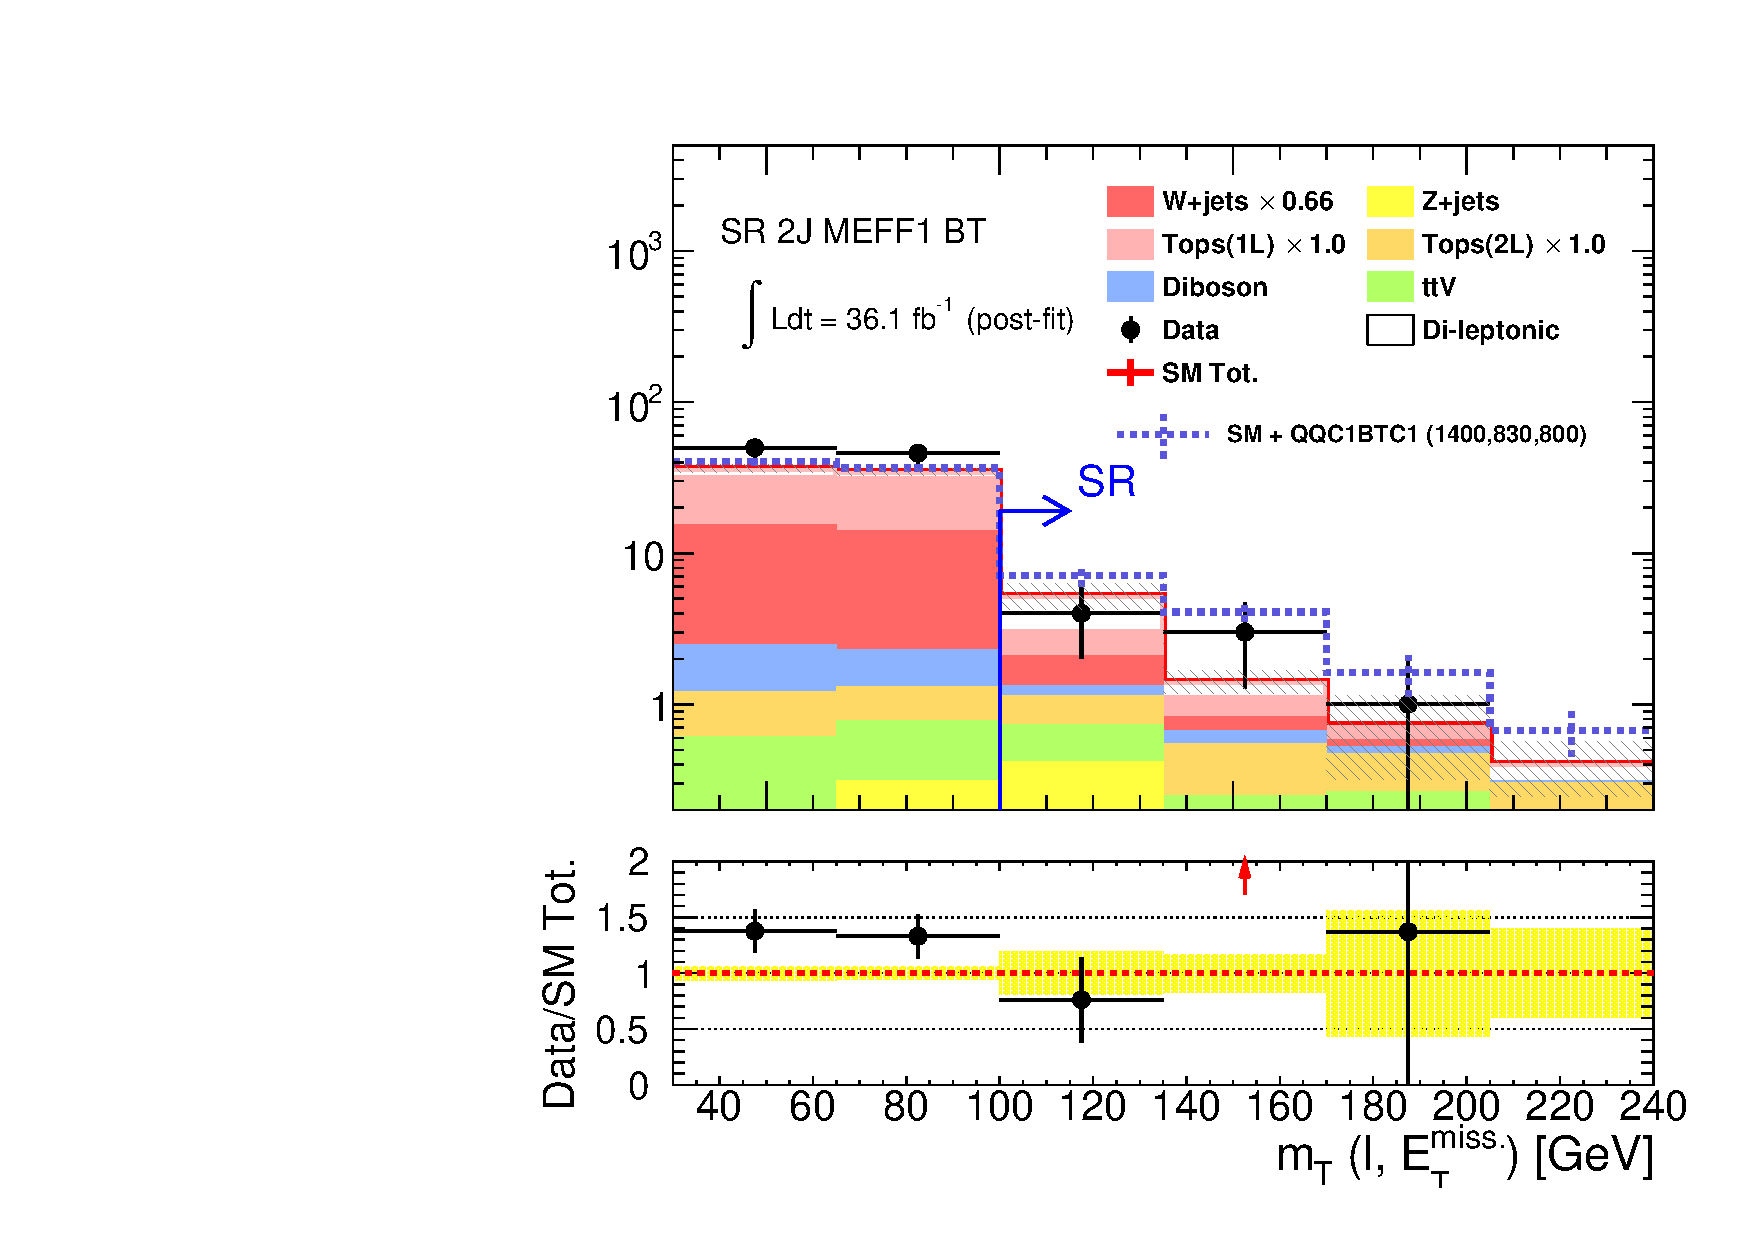
\includegraphics[width=0.41\textwidth]{figures/BGestimation/SRVRpostFit/mt__SR2JMEFF1BT_no_mt_postFit_2SFconfig_noYields_objRep.pdf}}
    \subfigure[]{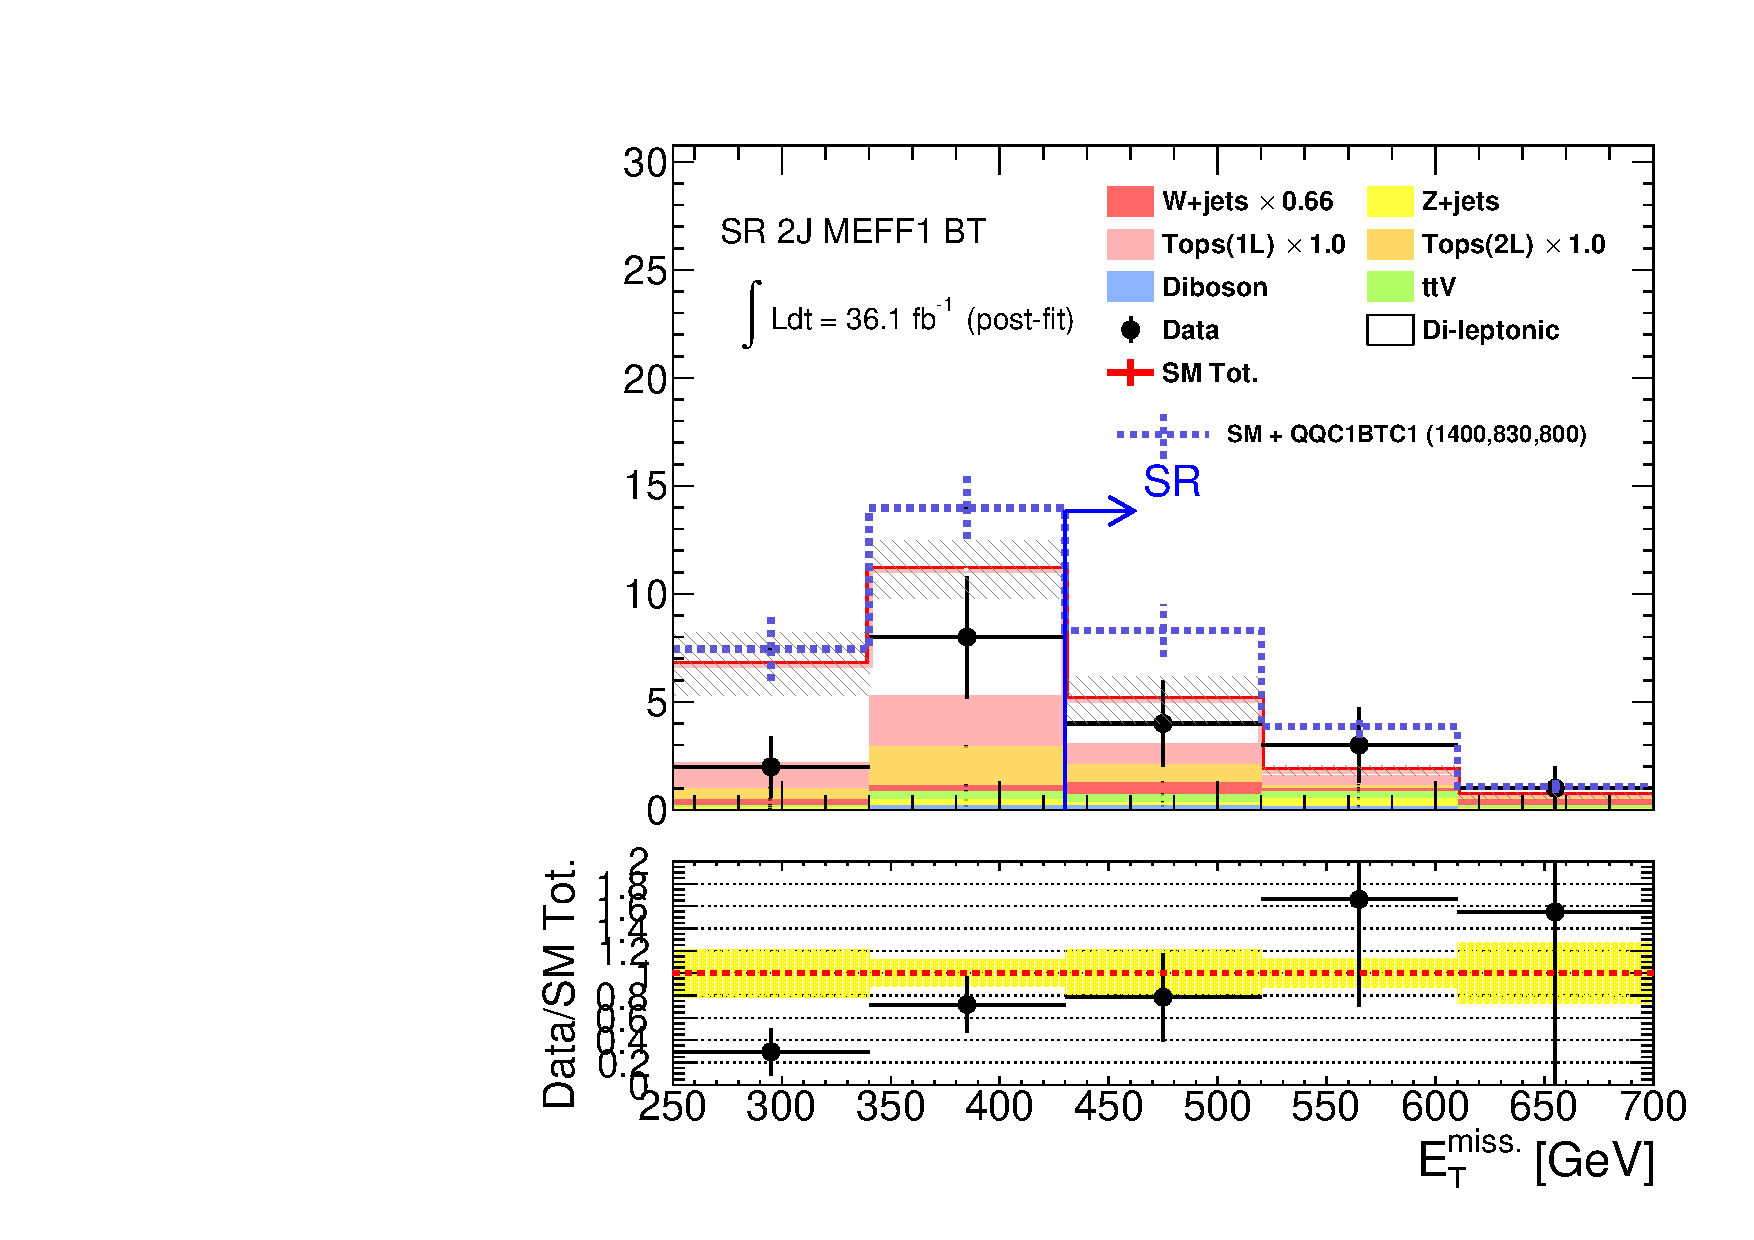
\includegraphics[width=0.41\textwidth]{figures/BGestimation/SRVRpostFit/met__SR2JMEFF1BT_no_met_postFit_2SFconfig_noYields_objRep.pdf}}
    \subfigure[]{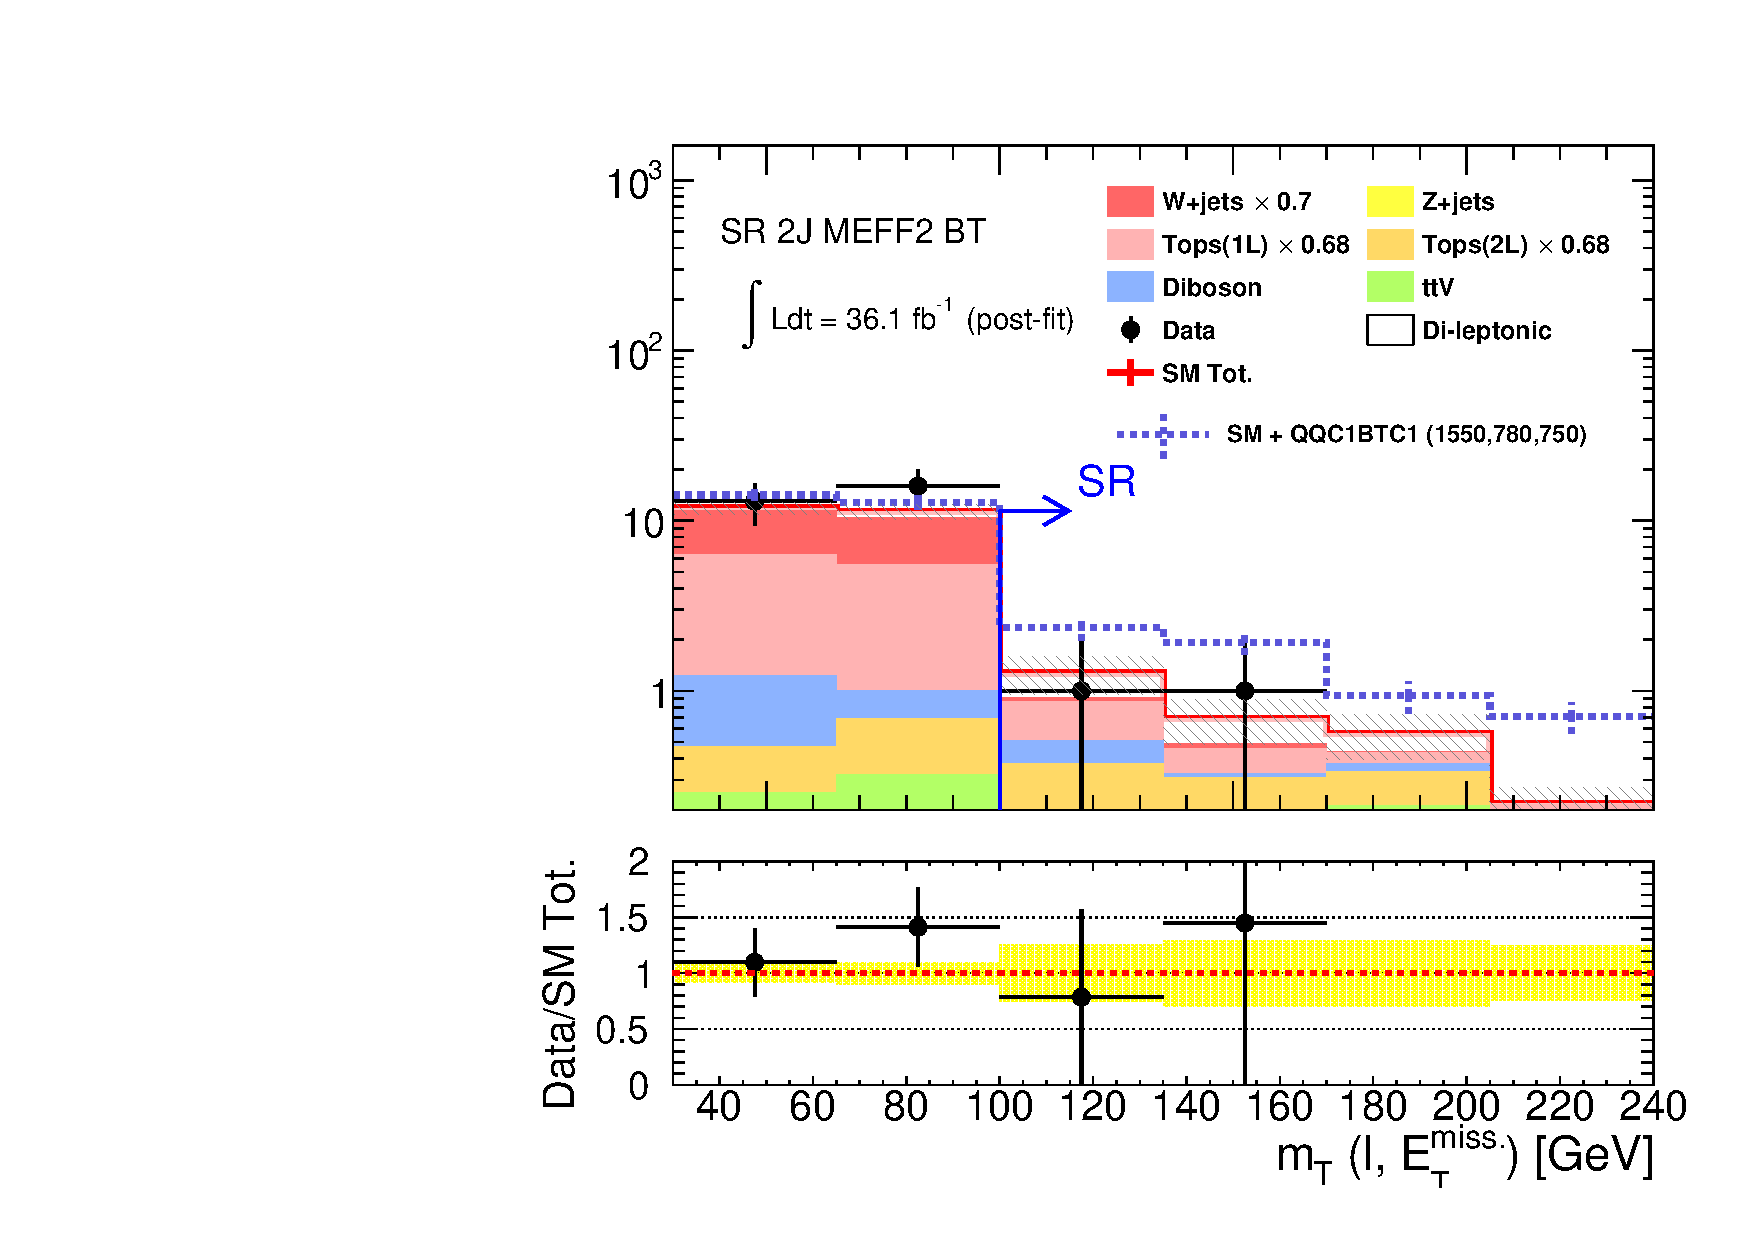
\includegraphics[width=0.41\textwidth]{figures/BGestimation/SRVRpostFit/mt__SR2JMEFF2BT_no_mt_postFit_2SFconfig_noYields_objRep.pdf}}
    \subfigure[]{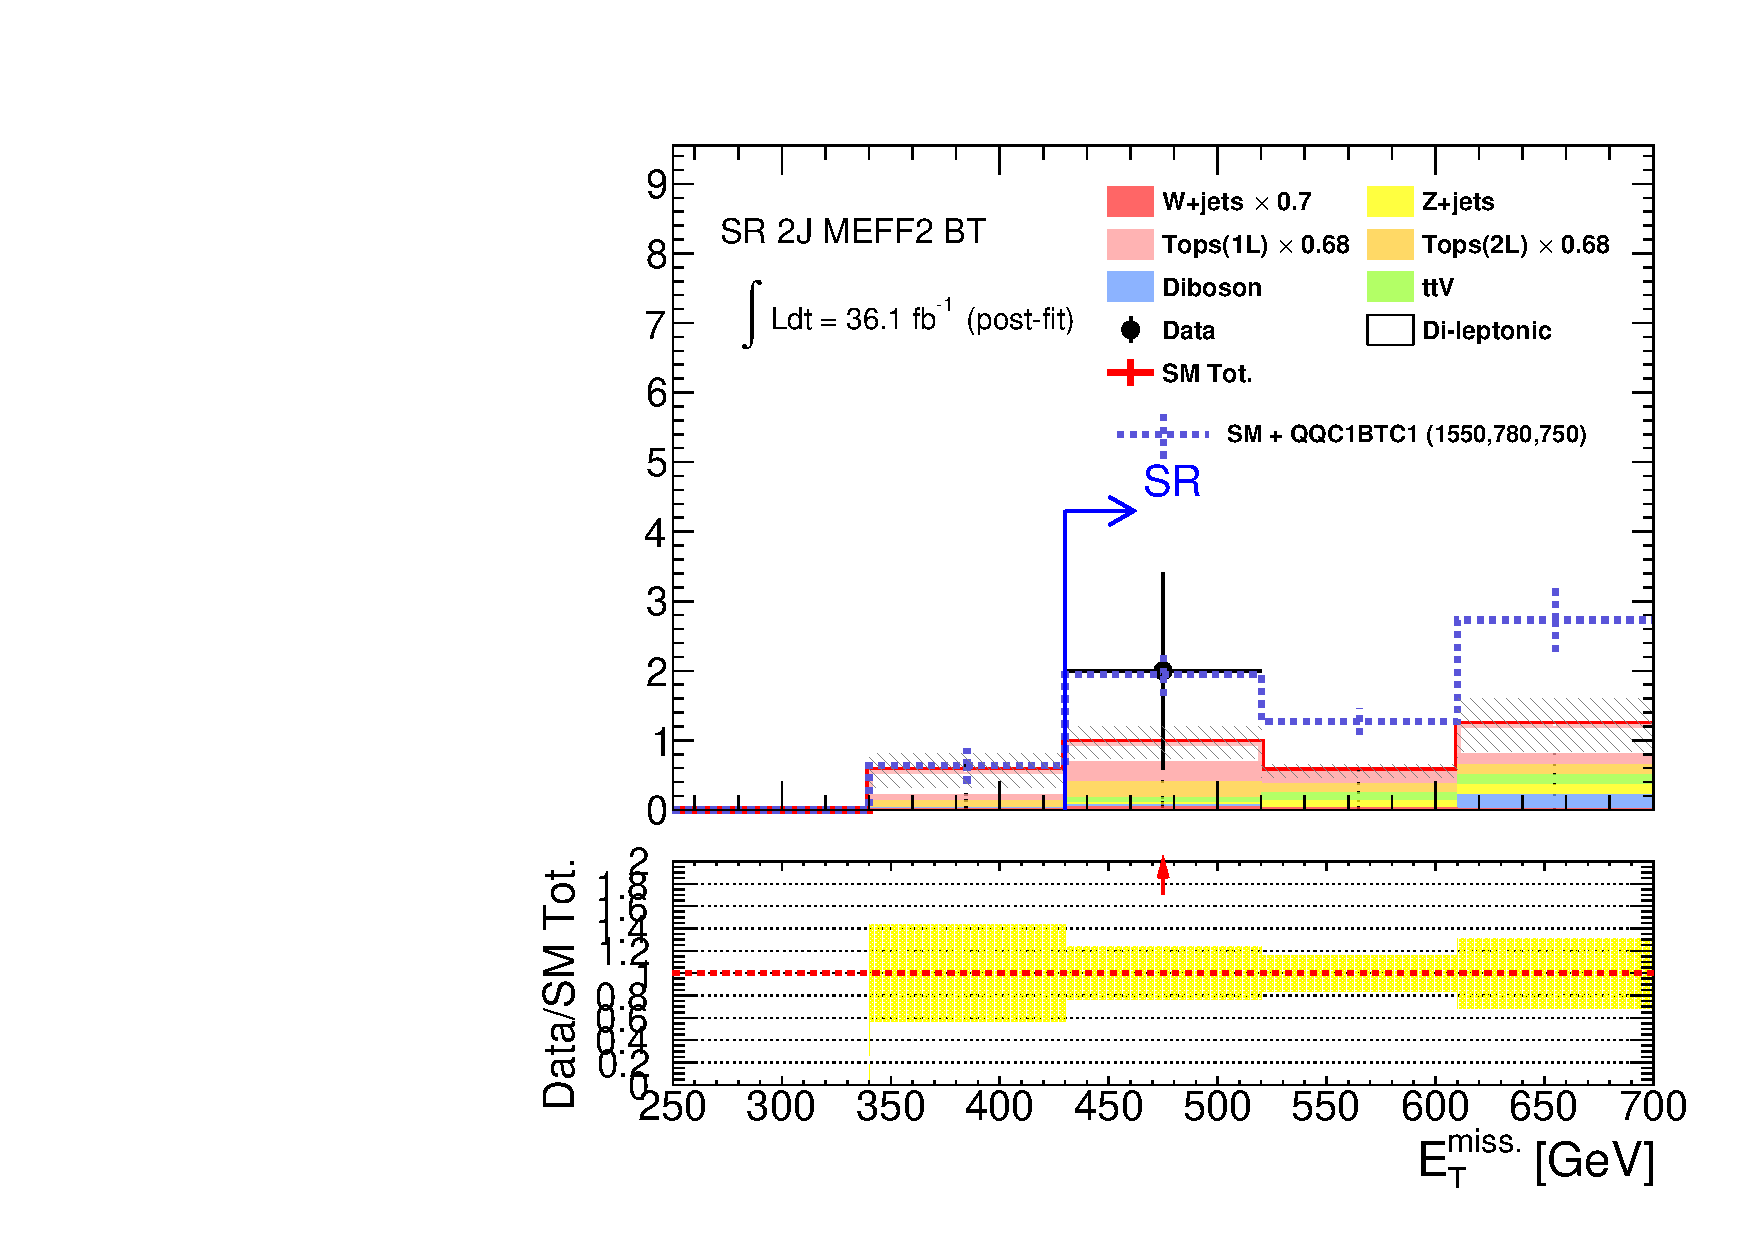
\includegraphics[width=0.41\textwidth]{figures/BGestimation/SRVRpostFit/met__SR2JMEFF2BT_no_met_postFit_2SFconfig_noYields_objRep.pdf}}
    \subfigure[]{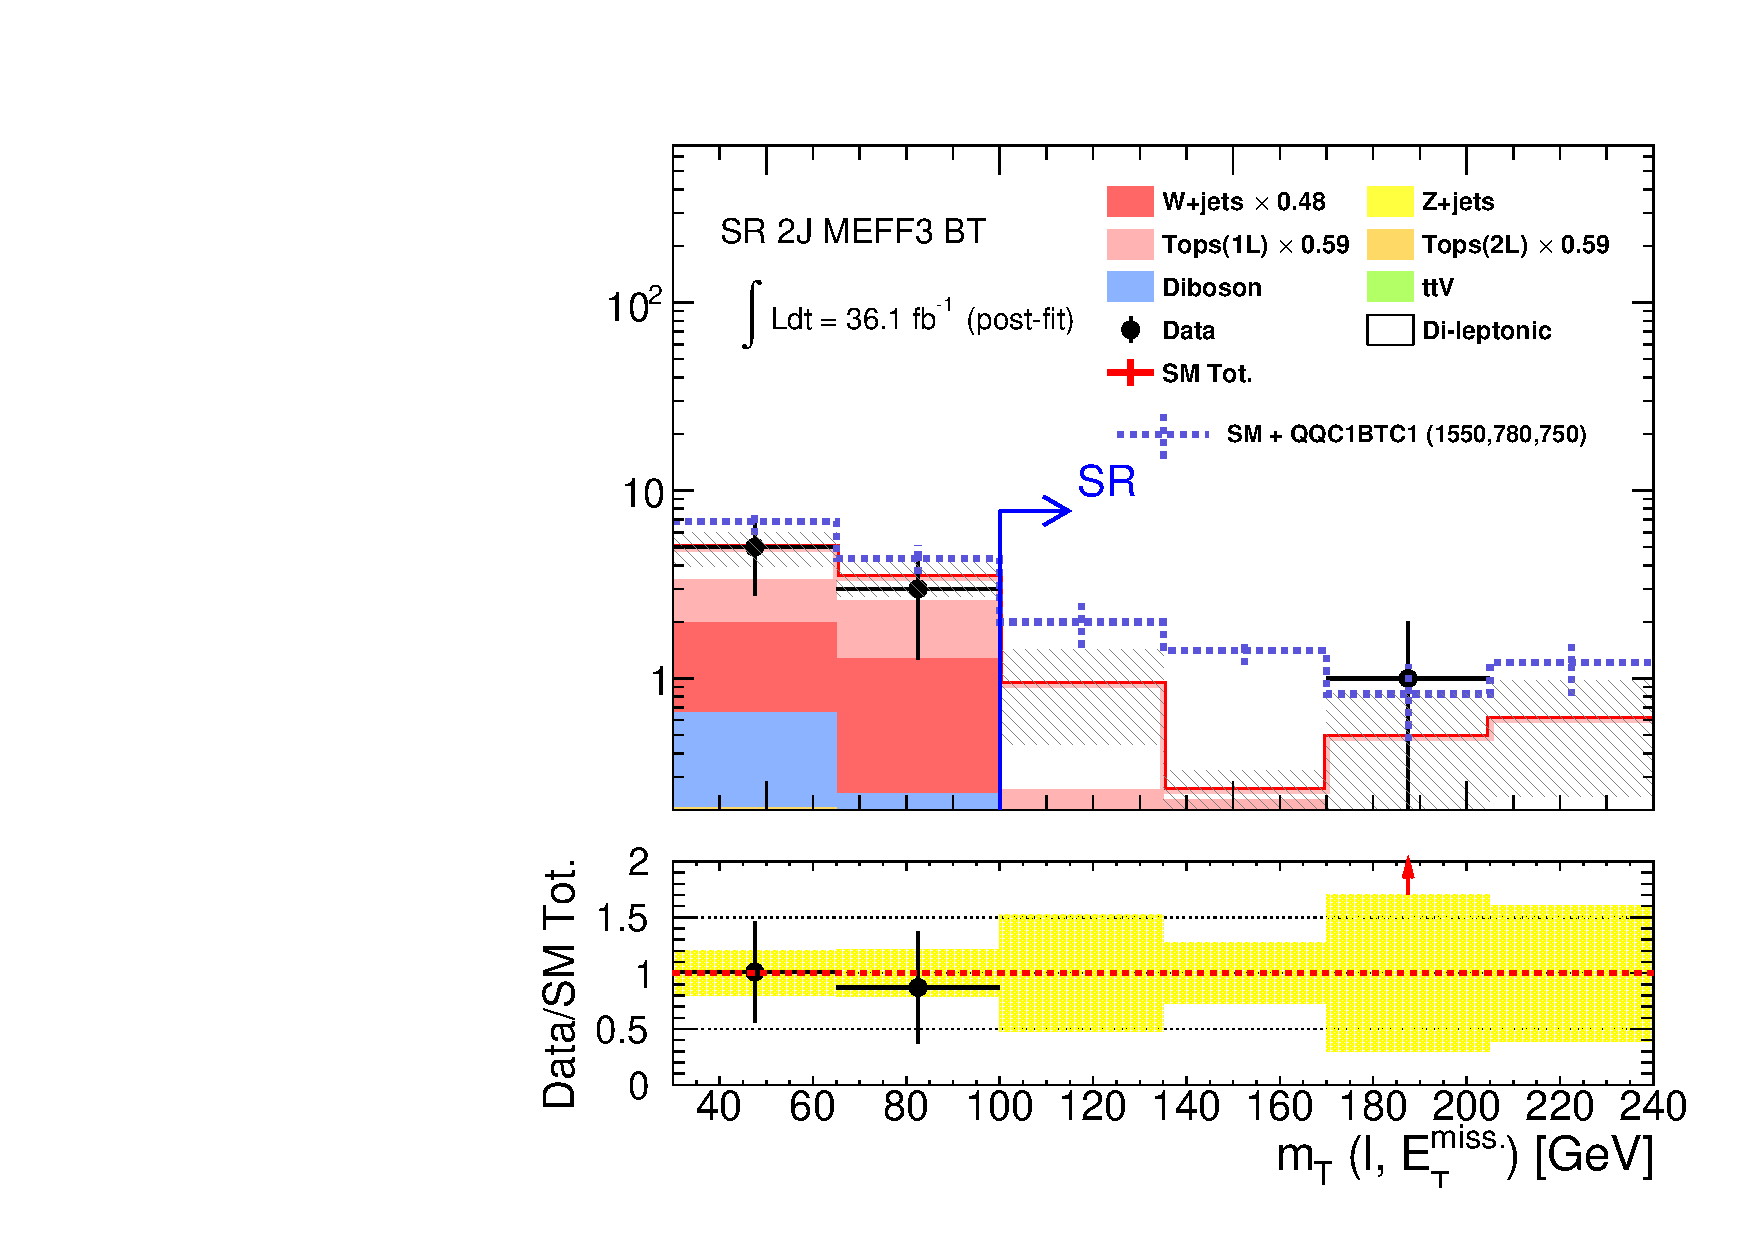
\includegraphics[width=0.41\textwidth]{figures/BGestimation/SRVRpostFit/mt__SR2JMEFF3BT_no_mt_postFit_2SFconfig_noYields_objRep.pdf}}
    \subfigure[]{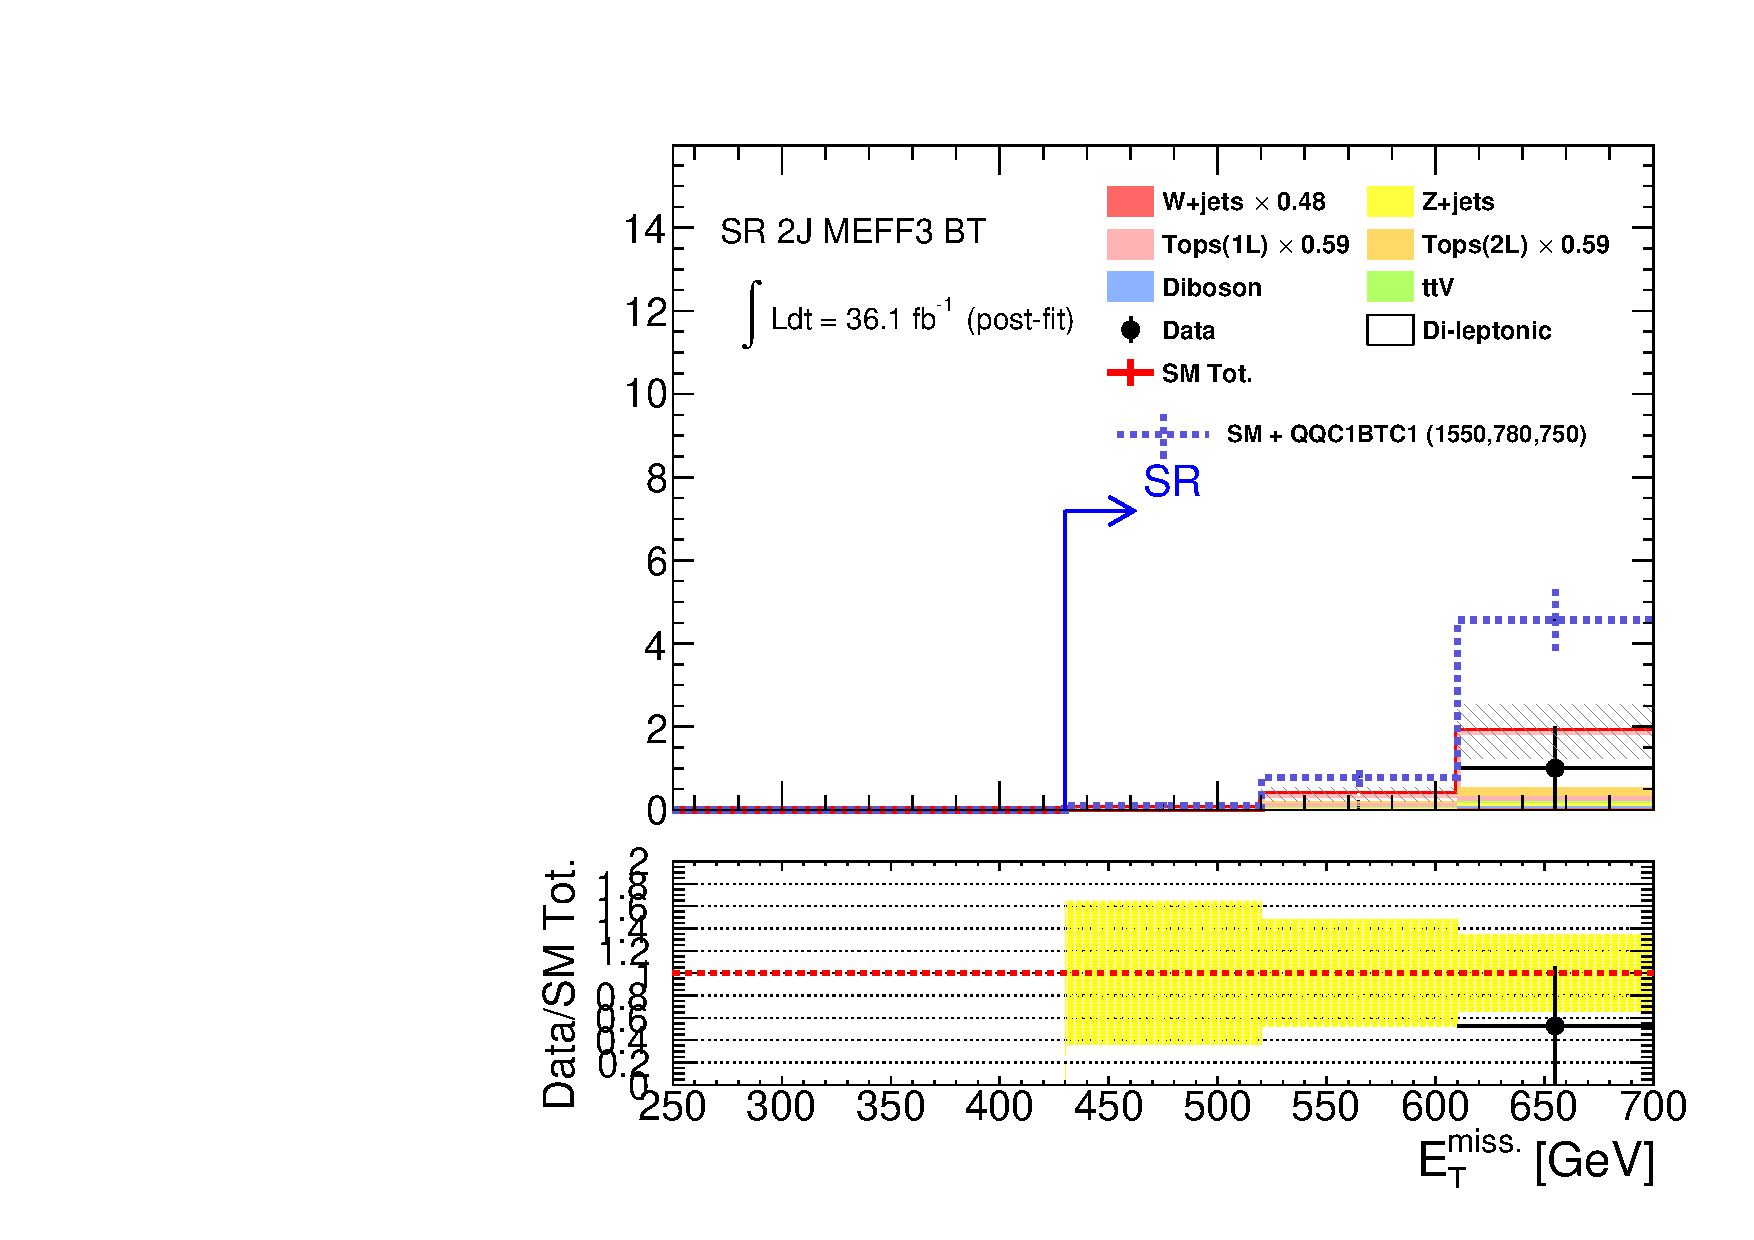
\includegraphics[width=0.41\textwidth]{figures/BGestimation/SRVRpostFit/met__SR2JMEFF3BT_no_met_postFit_2SFconfig_noYields_objRep.pdf}}
   \caption{
     Post-fit distruibution of (left) $\mt$, and (right) $\met$.
     (a,b) SR 2J-$\meffIncFirst$ BT.
     (c,d) SR 2J-$\meffIncSecond$ BT.
     (e,f) SR 2J-$\meffIncThird$ BT. 
     The yellow band in the bottom panel represents statistical error. The overflow is included in the highest bin.  
     \label{fig::BGestimation::SRVRpostFit::SR2JBT}
   }
\end{figure}


\clearpage
\begin{figure}[h]
  \centering
    \subfigure[]{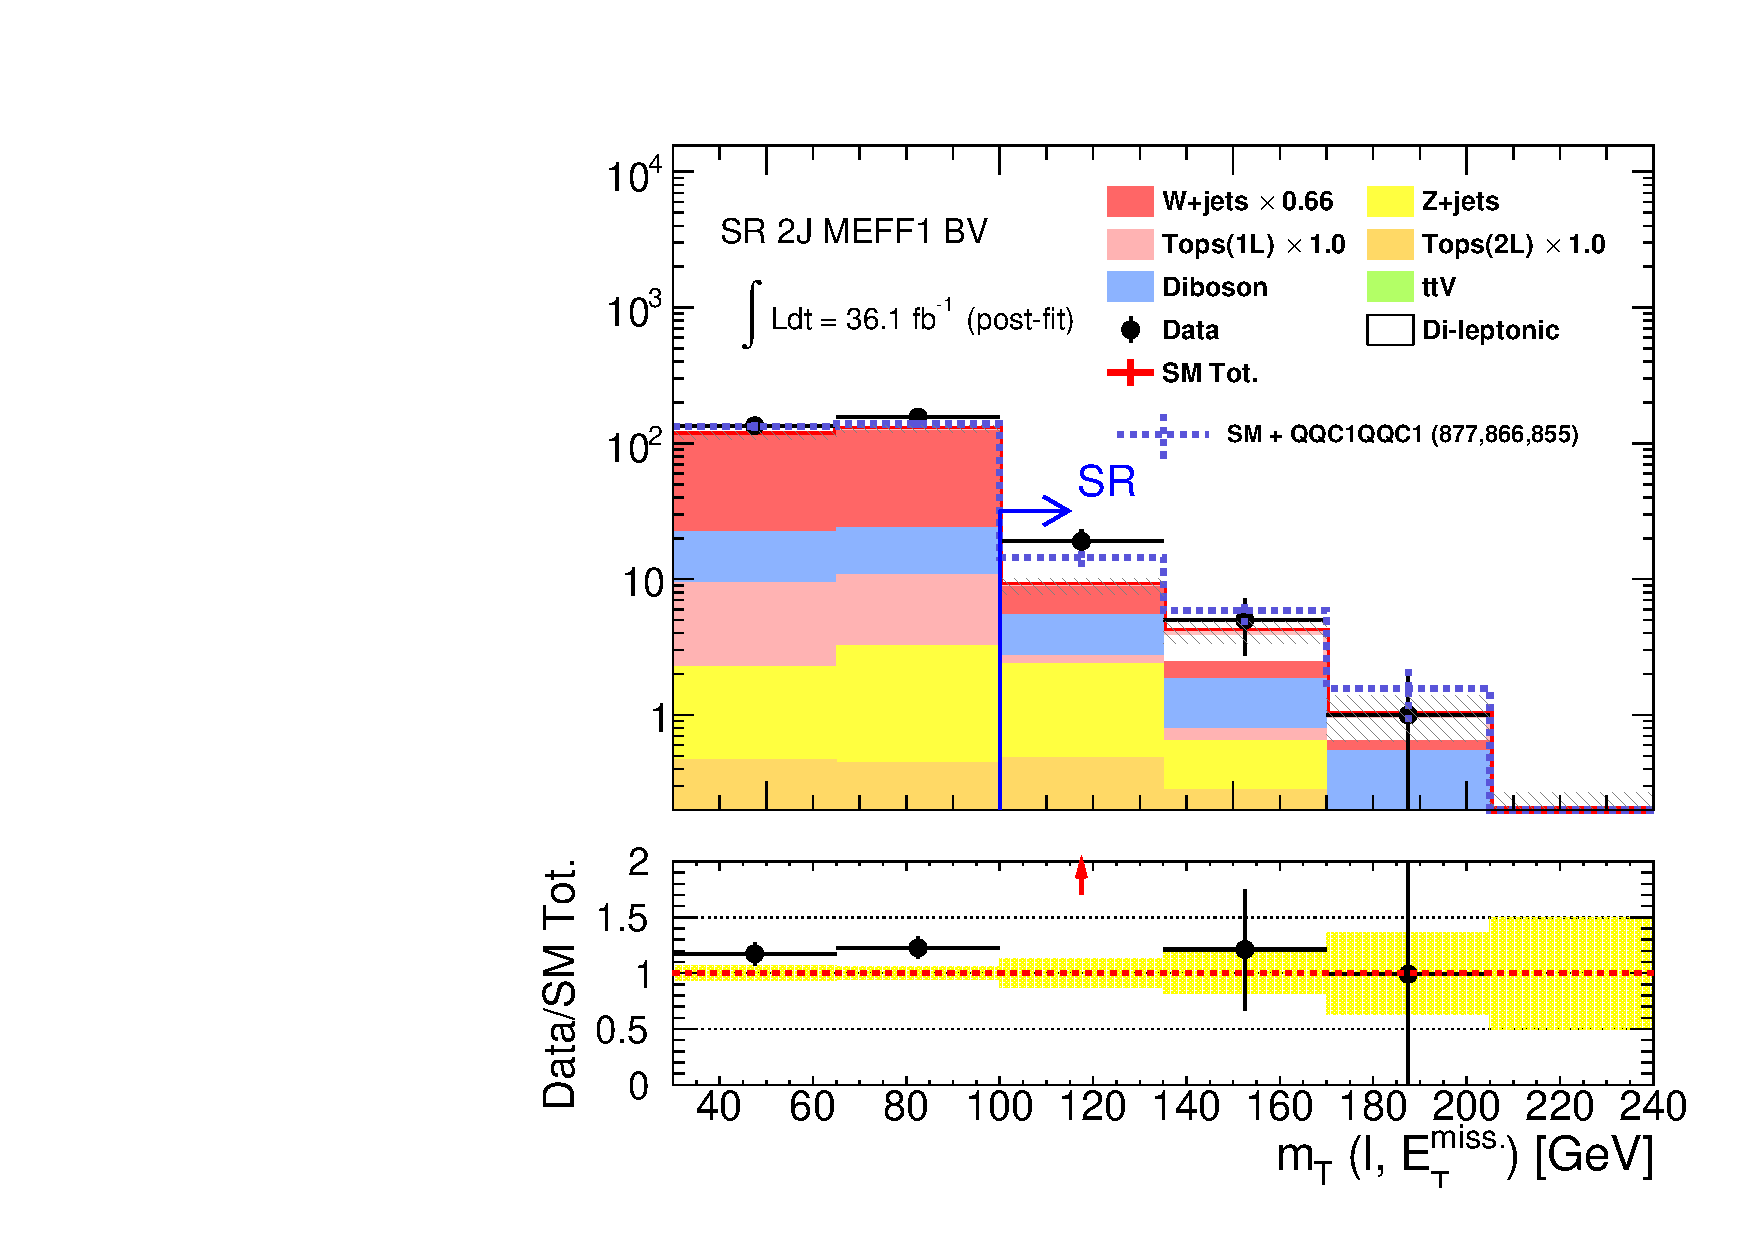
\includegraphics[width=0.41\textwidth]{figures/BGestimation/SRVRpostFit/mt__SR2JMEFF1BV_no_mt_postFit_2SFconfig_noYields_objRep.pdf}}
    \subfigure[]{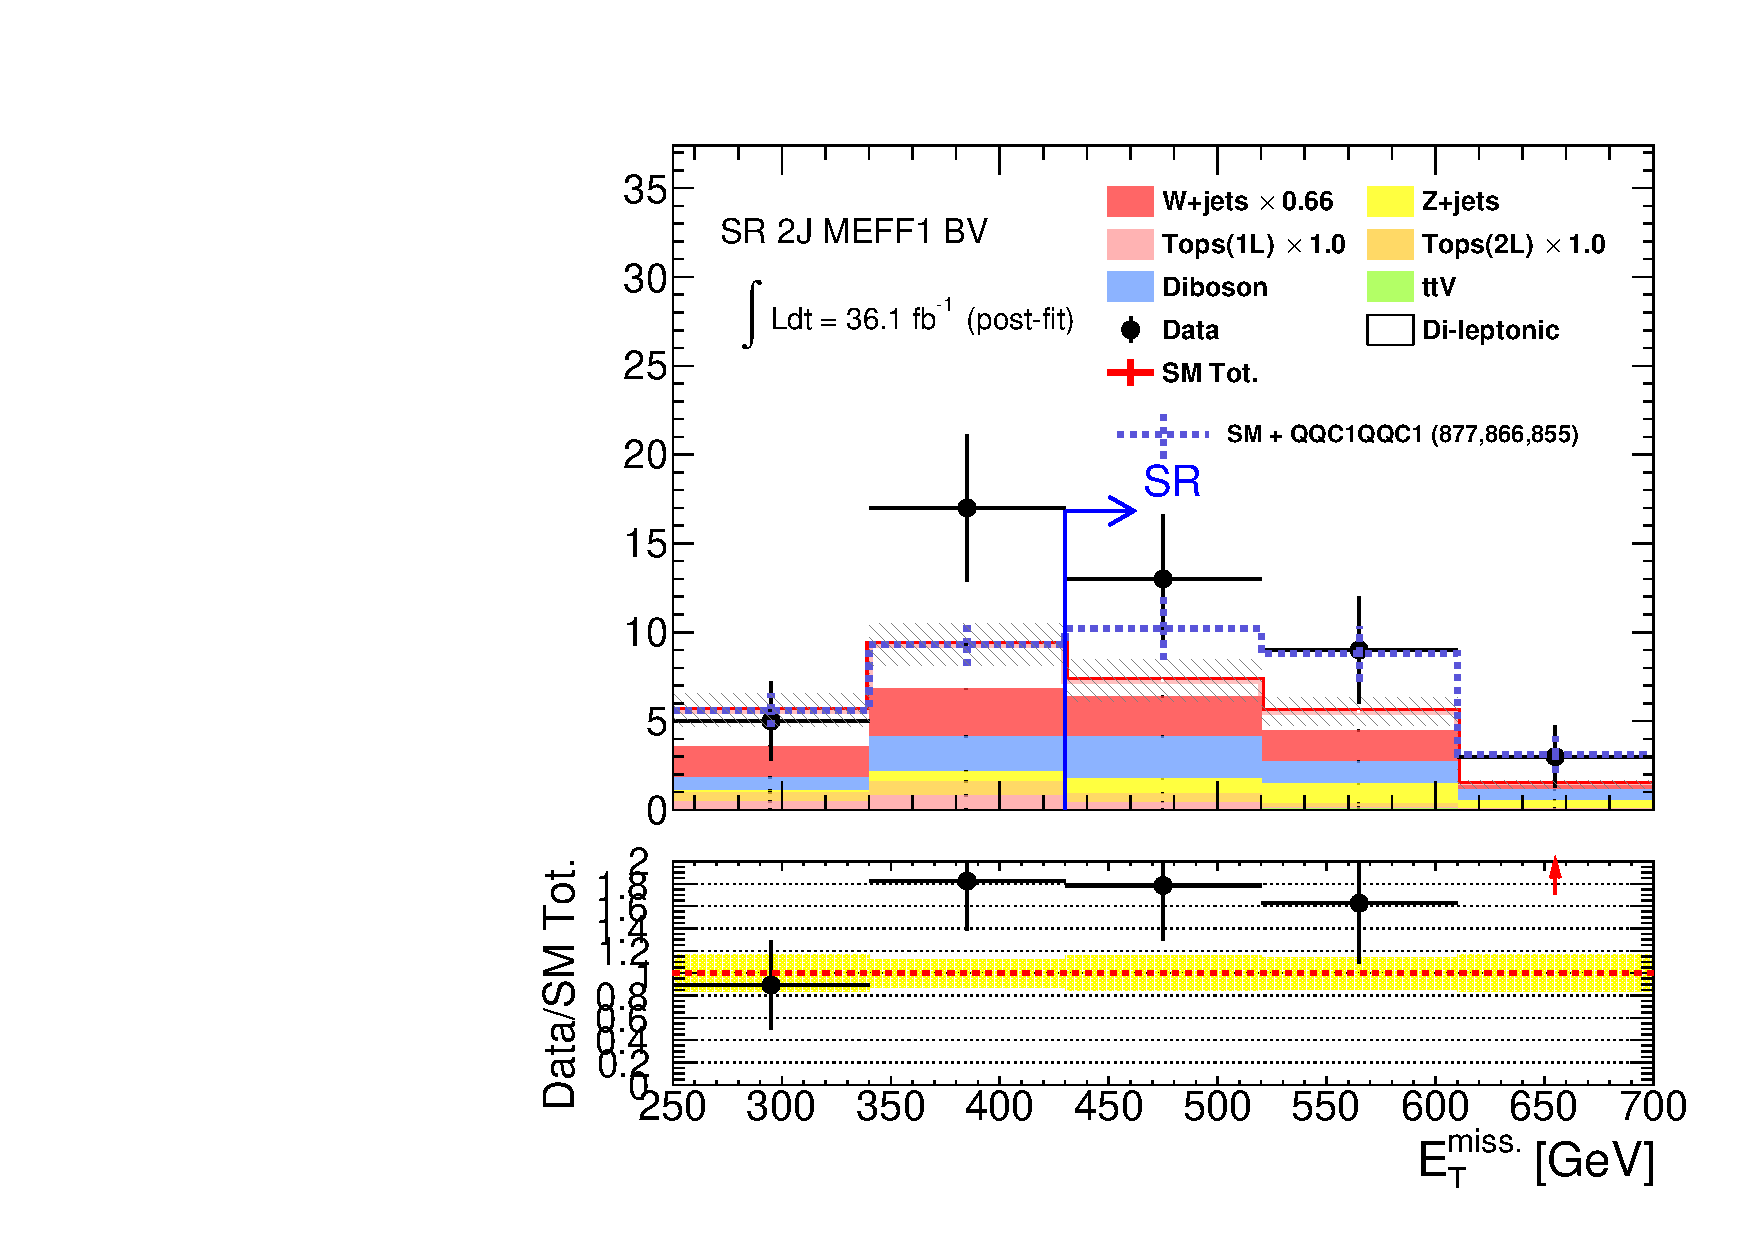
\includegraphics[width=0.41\textwidth]{figures/BGestimation/SRVRpostFit/met__SR2JMEFF1BV_no_met_postFit_2SFconfig_noYields_objRep.pdf}}
    \subfigure[]{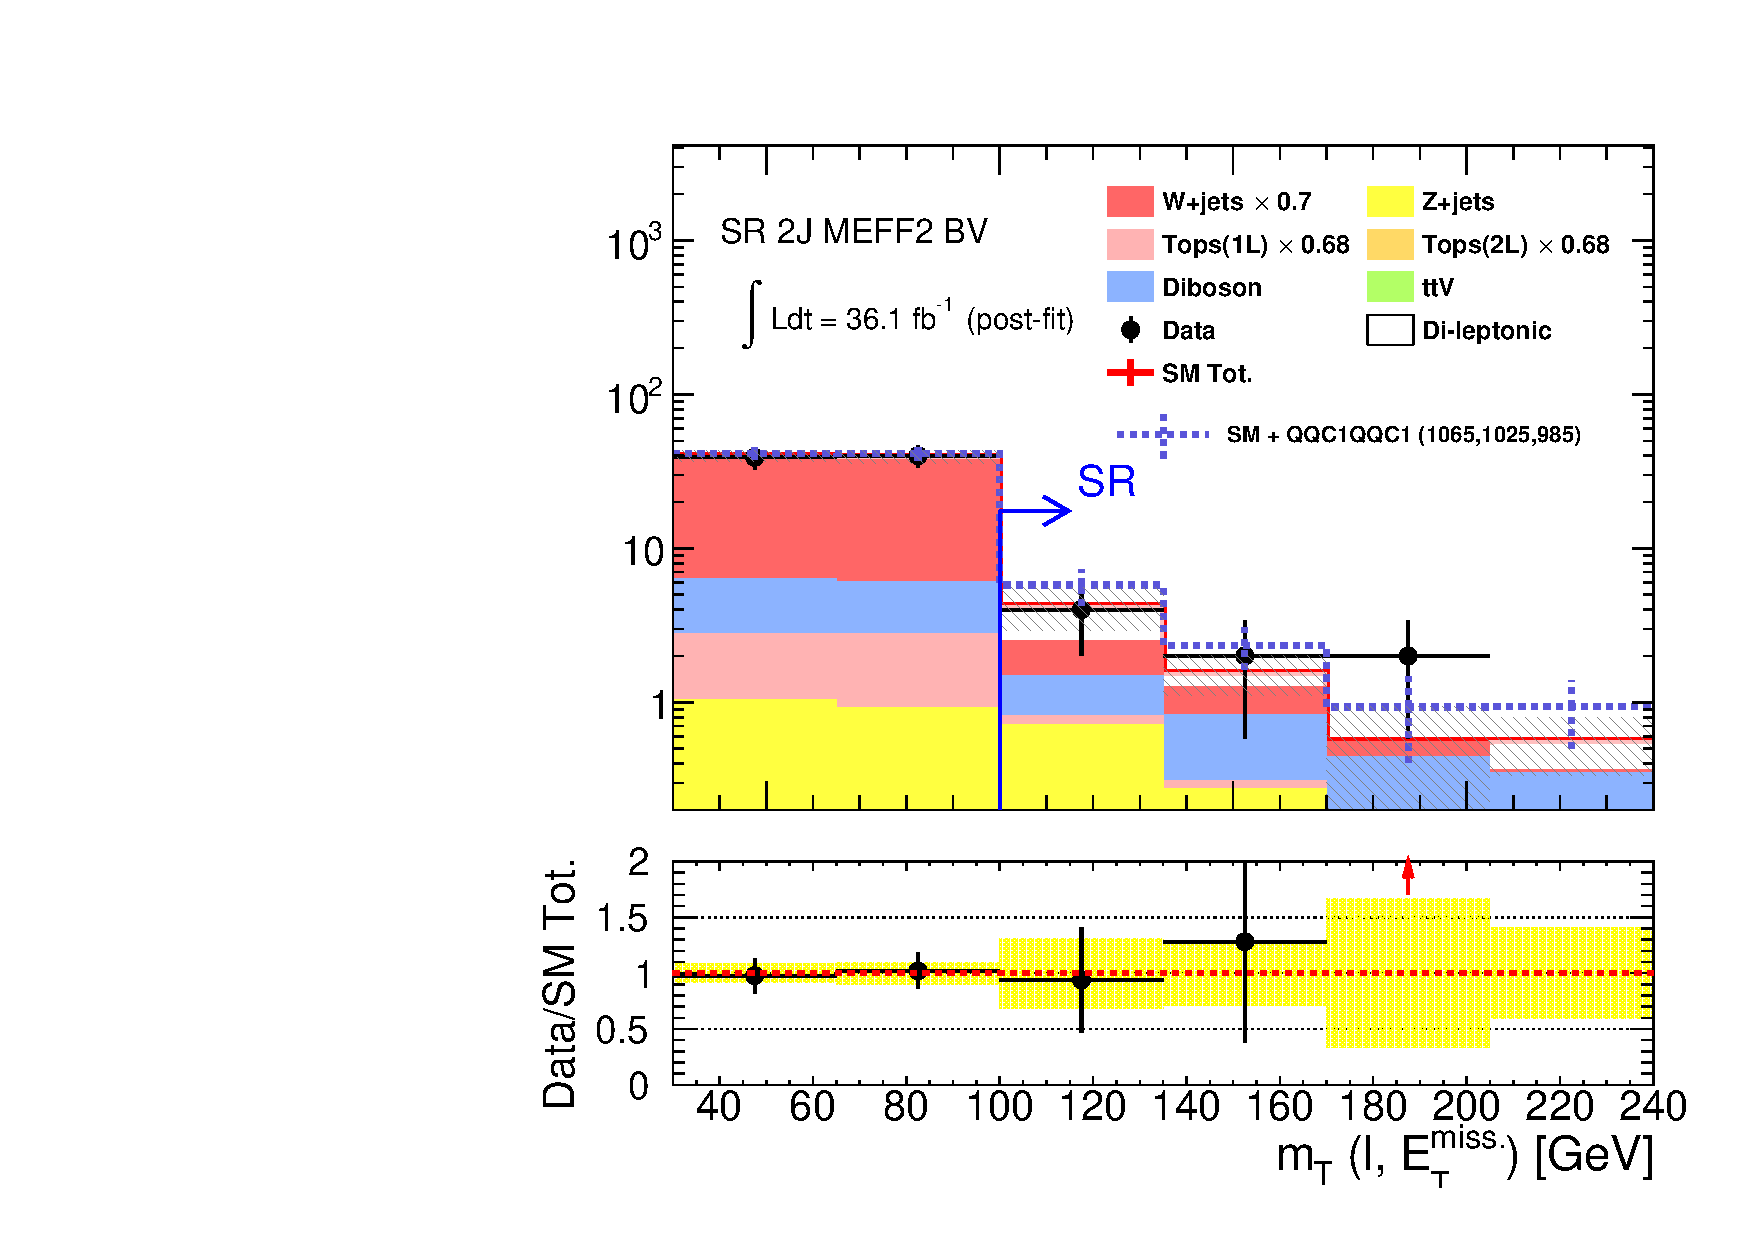
\includegraphics[width=0.41\textwidth]{figures/BGestimation/SRVRpostFit/mt__SR2JMEFF2BV_no_mt_postFit_2SFconfig_noYields_objRep.pdf}}
    \subfigure[]{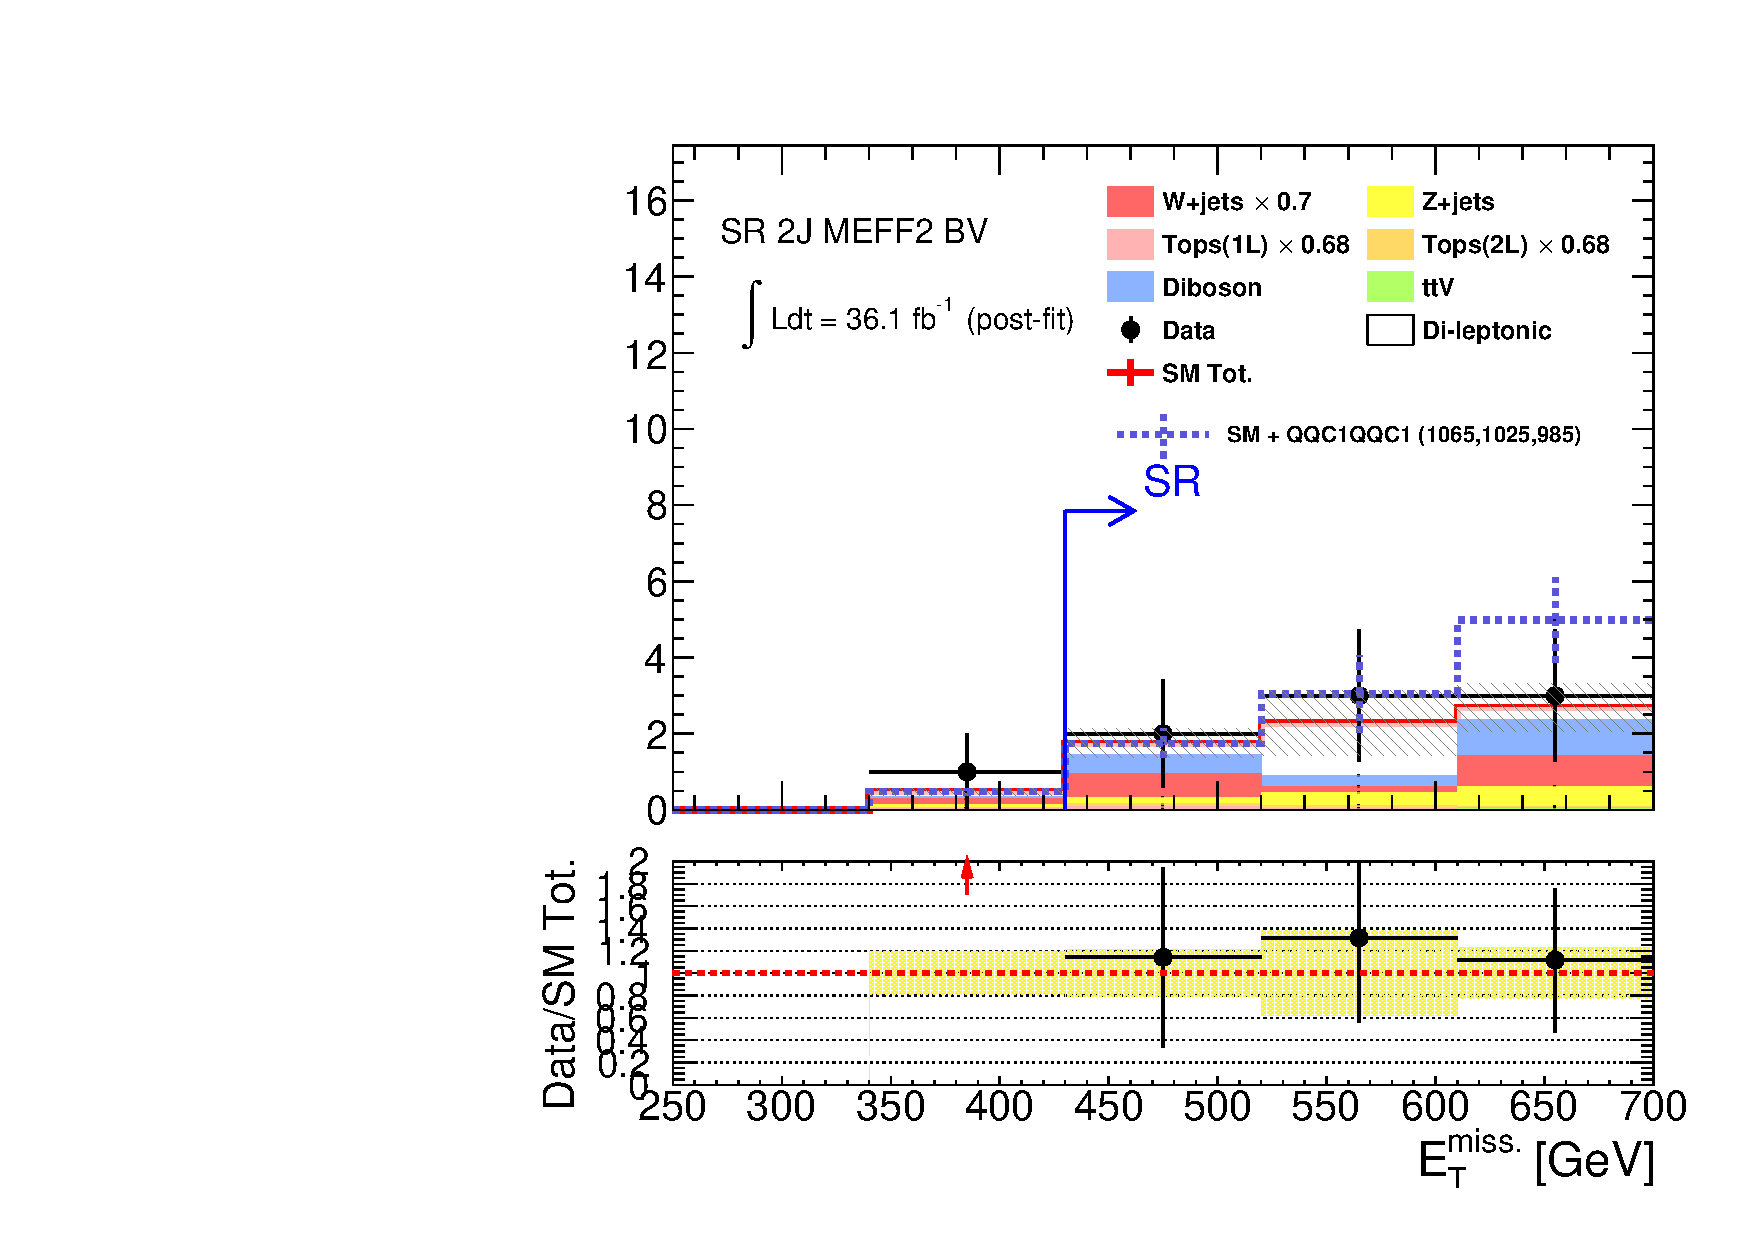
\includegraphics[width=0.41\textwidth]{figures/BGestimation/SRVRpostFit/met__SR2JMEFF2BV_no_met_postFit_2SFconfig_noYields_objRep.pdf}}
    \subfigure[]{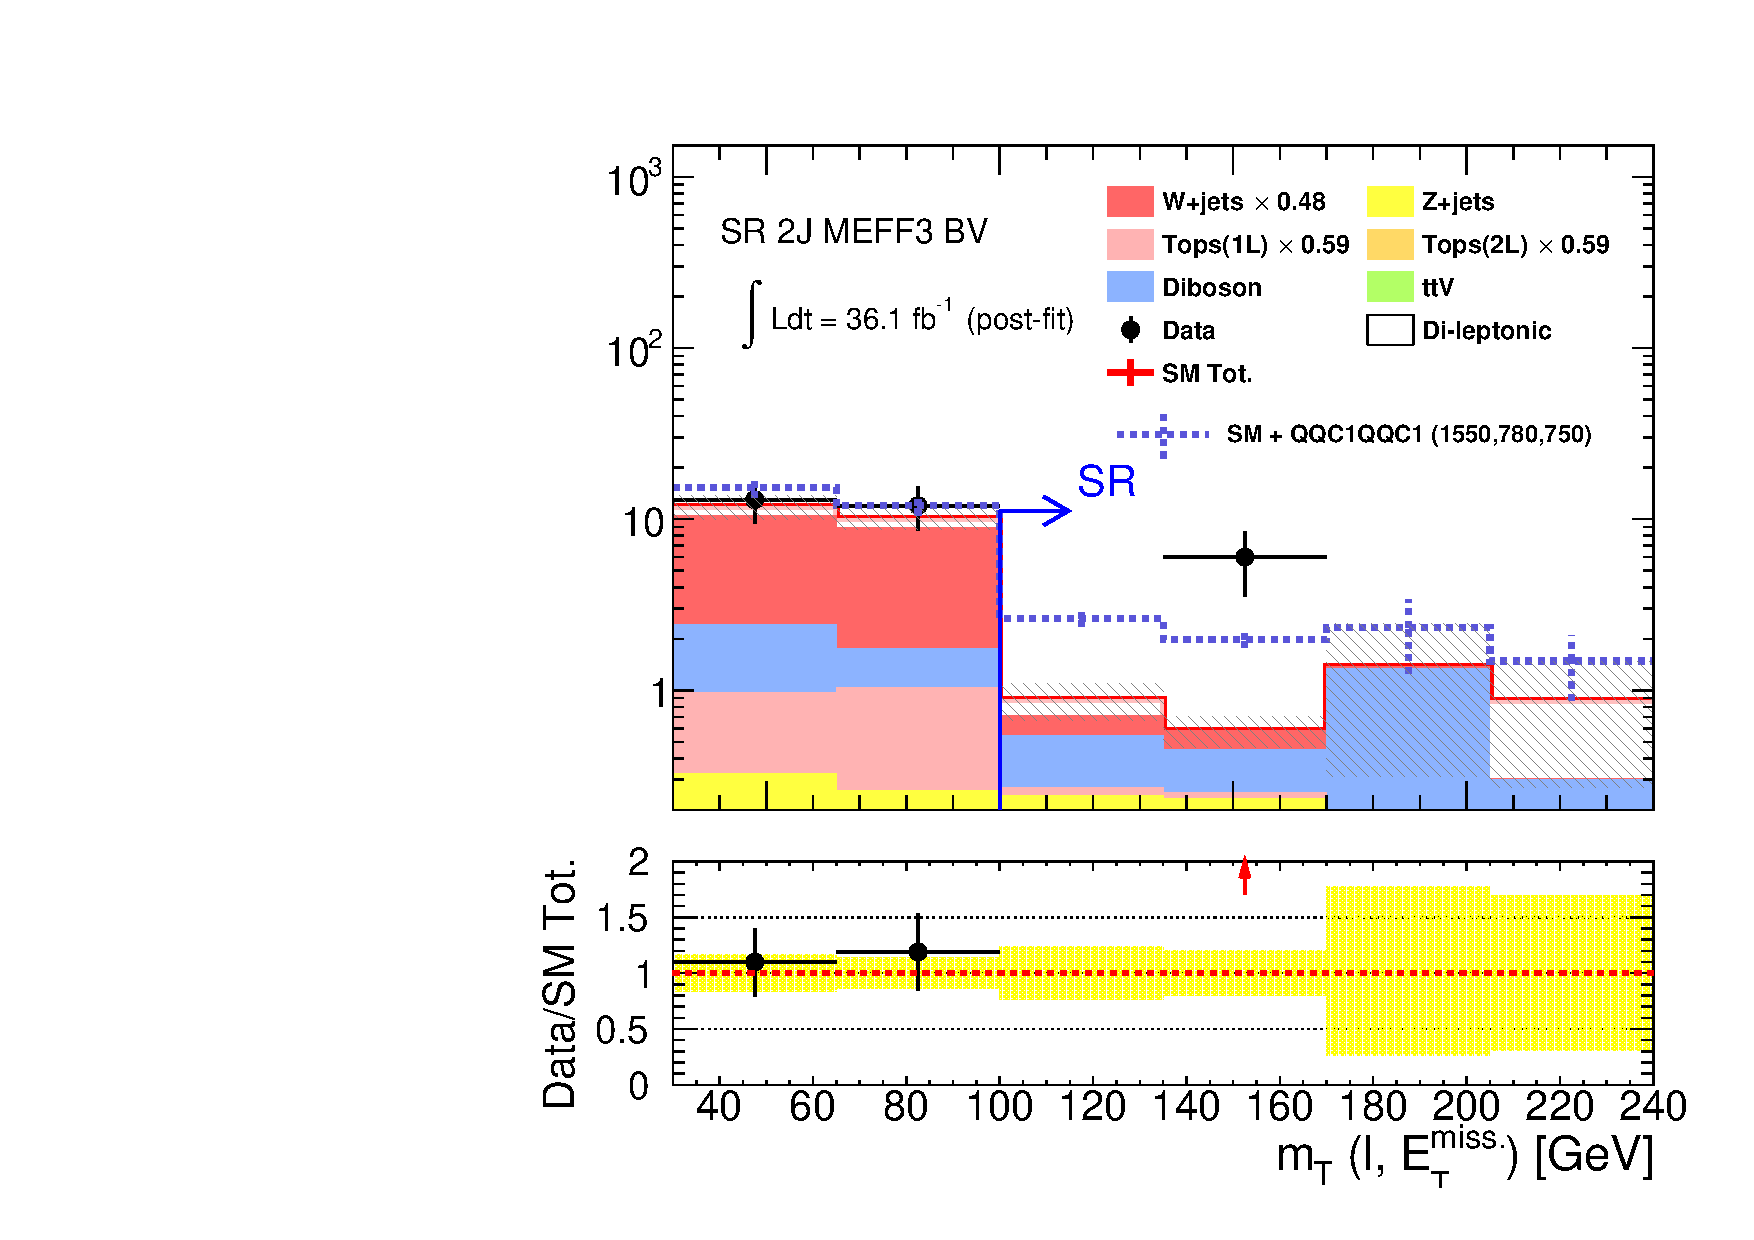
\includegraphics[width=0.41\textwidth]{figures/BGestimation/SRVRpostFit/mt__SR2JMEFF3BV_no_mt_postFit_2SFconfig_noYields_objRep.pdf}}
    \subfigure[]{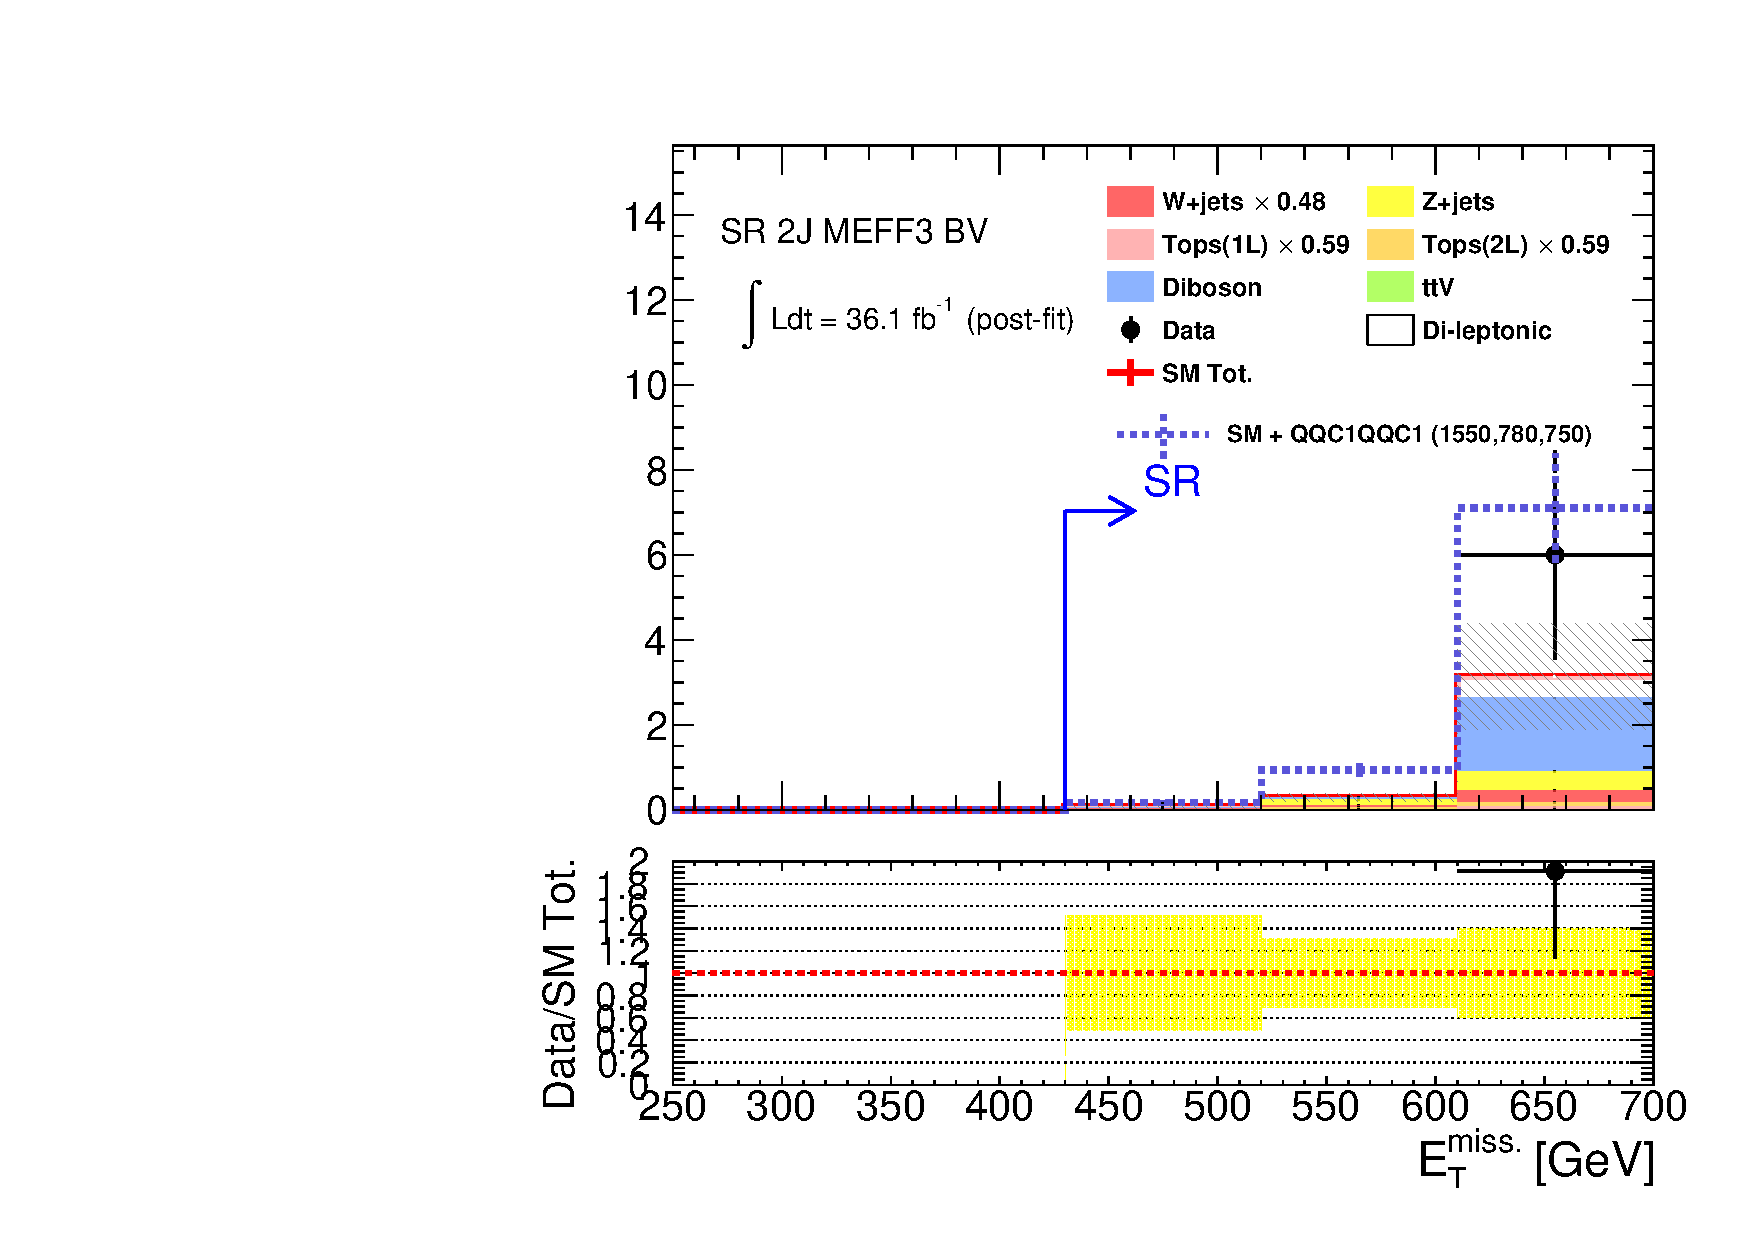
\includegraphics[width=0.41\textwidth]{figures/BGestimation/SRVRpostFit/met__SR2JMEFF3BV_no_met_postFit_2SFconfig_noYields_objRep.pdf}}
   \caption{
     Post-fit distruibution of (left) $\mt$, and (right) $\met$.
     (a,b) SR 2J-$\meffIncFirst$ BV.
     (c,d) SR 2J-$\meffIncSecond$ BV.
     (e,f) SR 2J-$\meffIncThird$ BV. 
     The yellow band in the bottom panel represents statistical error. The overflow is included in the highest bin.  
     \label{fig::BGestimation::SRVRpostFit::SR2JBV}
   }
\end{figure}
% -------------------------------------



\clearpage
% -------------- 6J ---------
\begin{figure}[h]
  \centering
    \subfigure[]{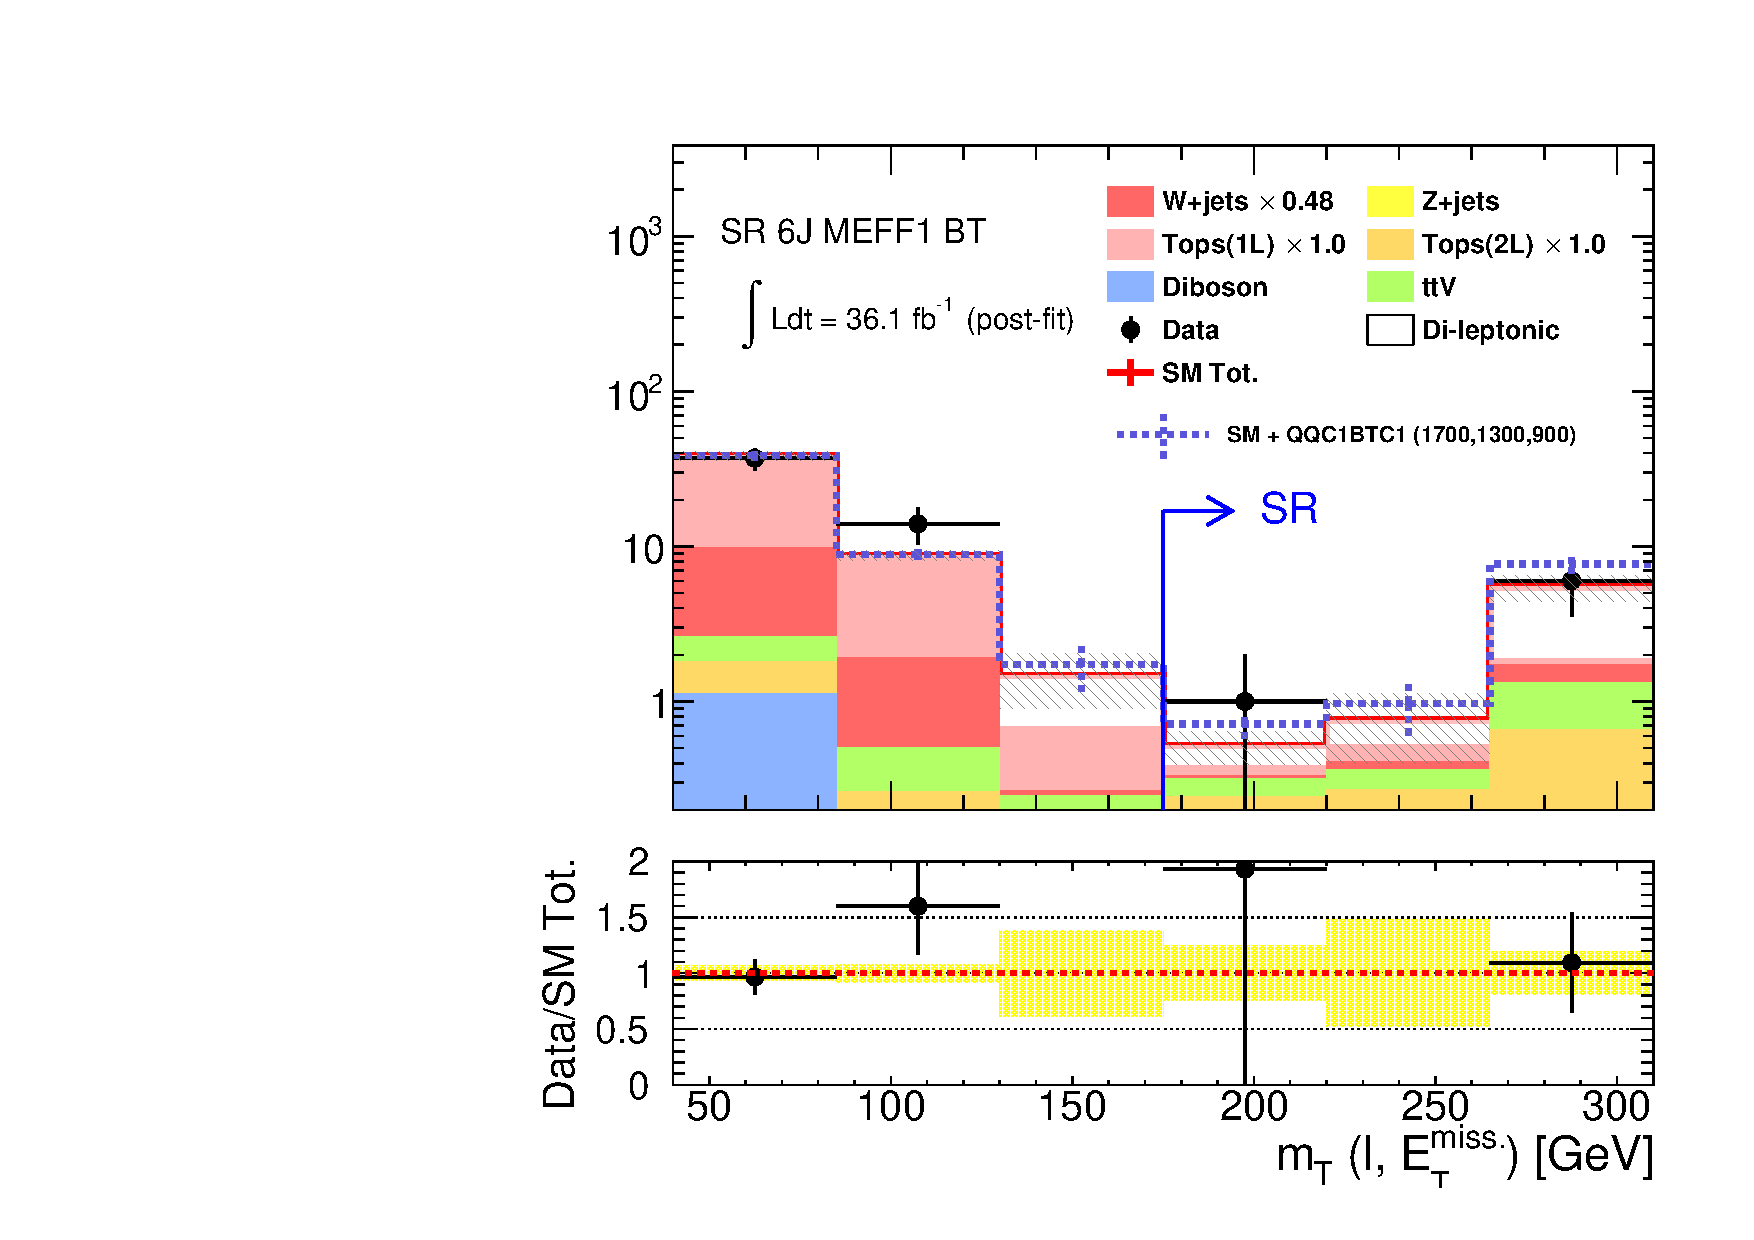
\includegraphics[width=0.41\textwidth]{figures/BGestimation/SRVRpostFit/mt__SR6JMEFF1BT_no_mt_postFit_2SFconfig_noYields_objRep.pdf}}
    \subfigure[]{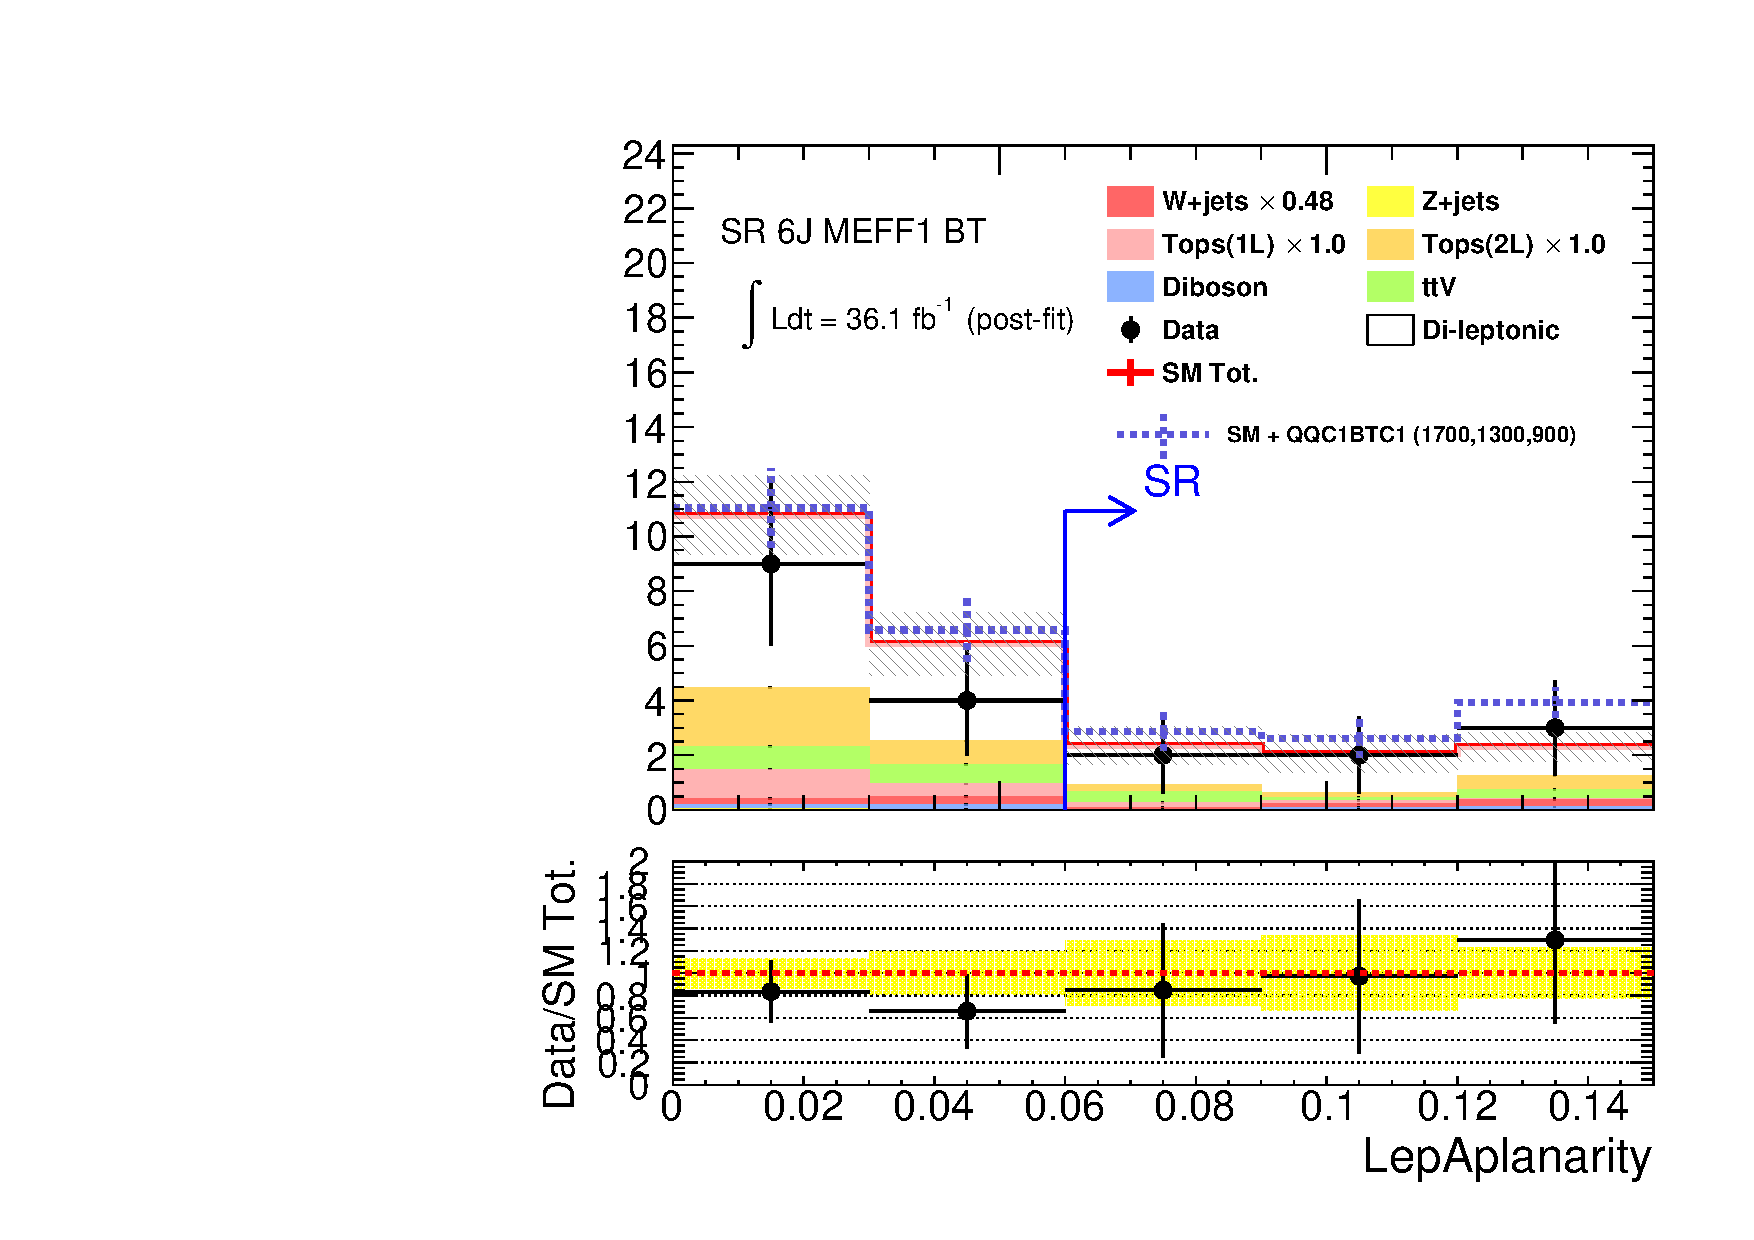
\includegraphics[width=0.41\textwidth]{figures/BGestimation/SRVRpostFit/LepAplanarity__SR6JMEFF1BT_no_LepAplanarity_postFit_2SFconfig_noYields_objRep.pdf}}
    \subfigure[]{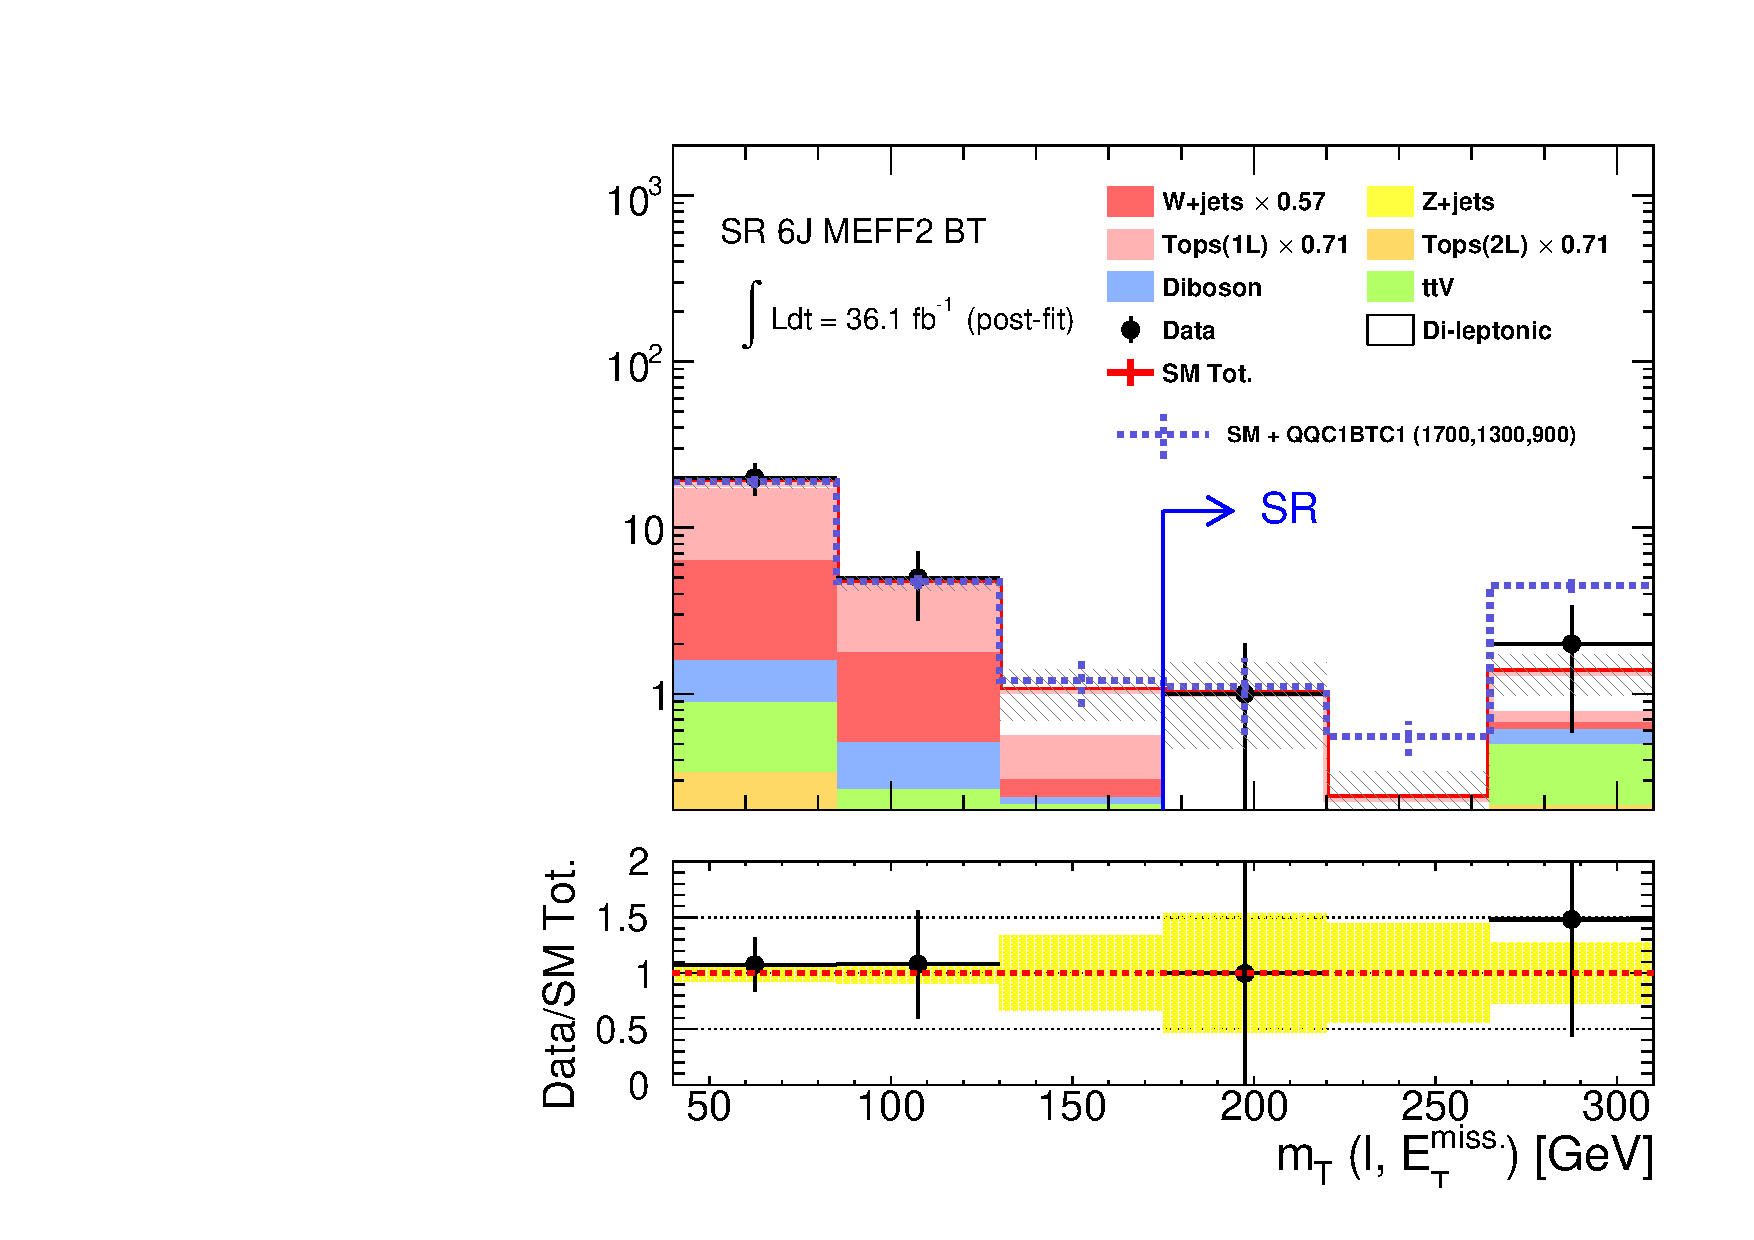
\includegraphics[width=0.41\textwidth]{figures/BGestimation/SRVRpostFit/mt__SR6JMEFF2BT_no_mt_postFit_2SFconfig_noYields_objRep.pdf}}
    \subfigure[]{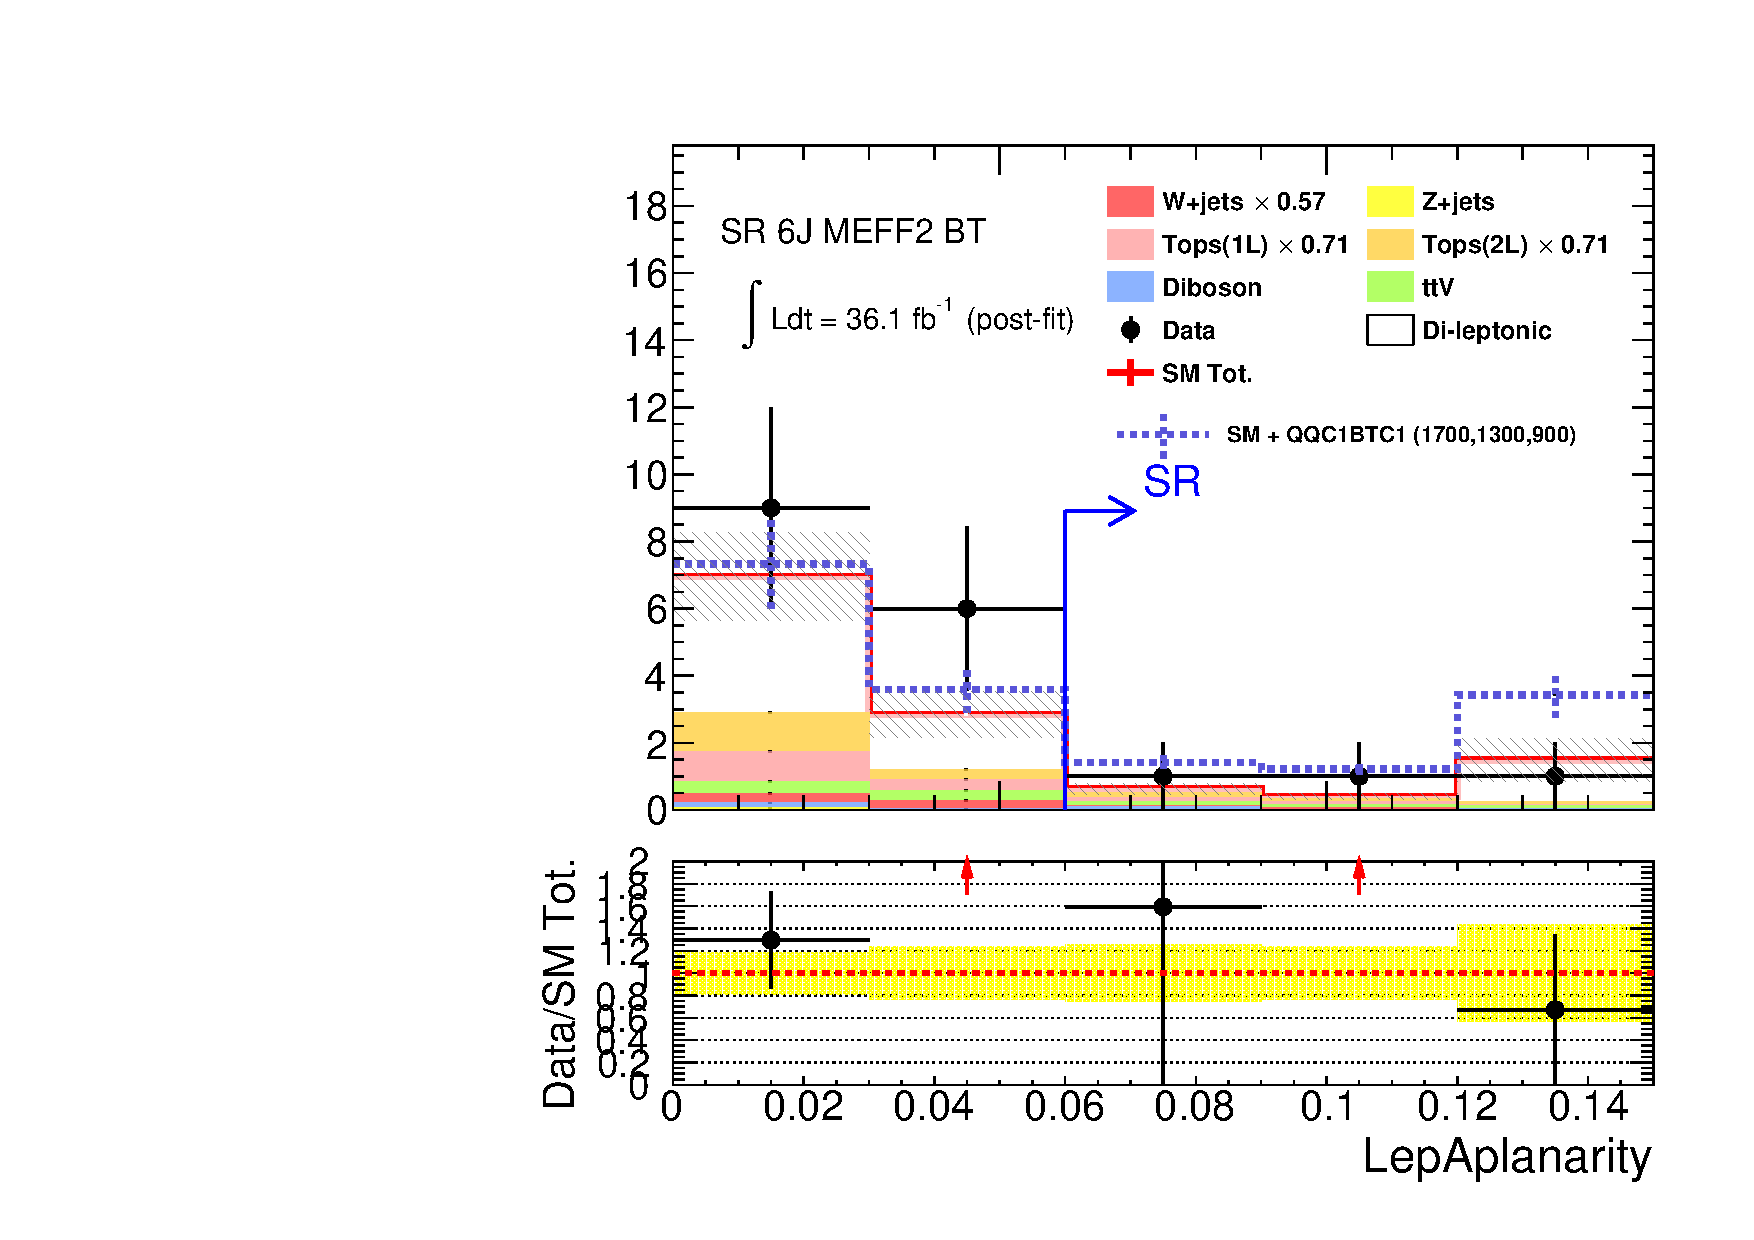
\includegraphics[width=0.41\textwidth]{figures/BGestimation/SRVRpostFit/LepAplanarity__SR6JMEFF2BT_no_LepAplanarity_postFit_2SFconfig_noYields_objRep.pdf}}
    \subfigure[]{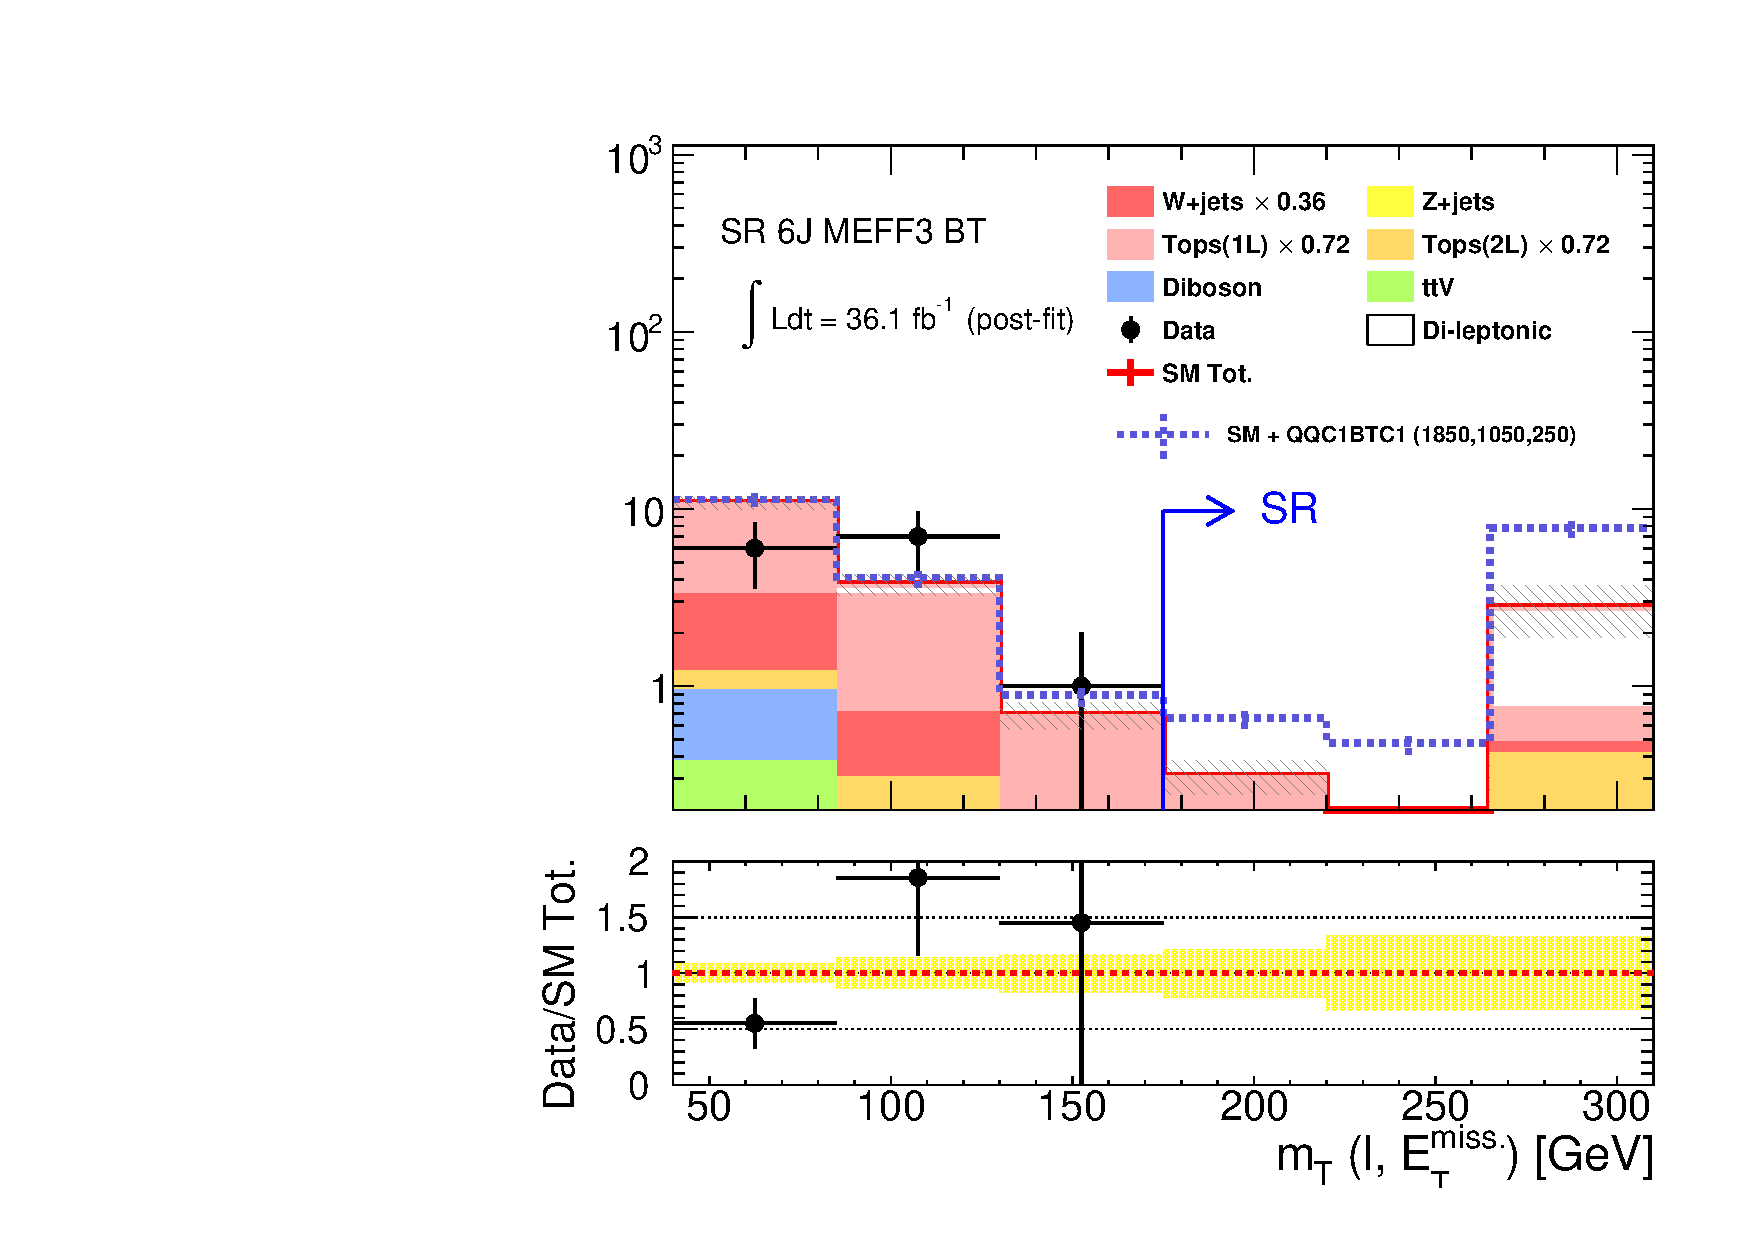
\includegraphics[width=0.41\textwidth]{figures/BGestimation/SRVRpostFit/mt__SR6JMEFF3BT_no_mt_postFit_2SFconfig_noYields_objRep.pdf}}
    \subfigure[]{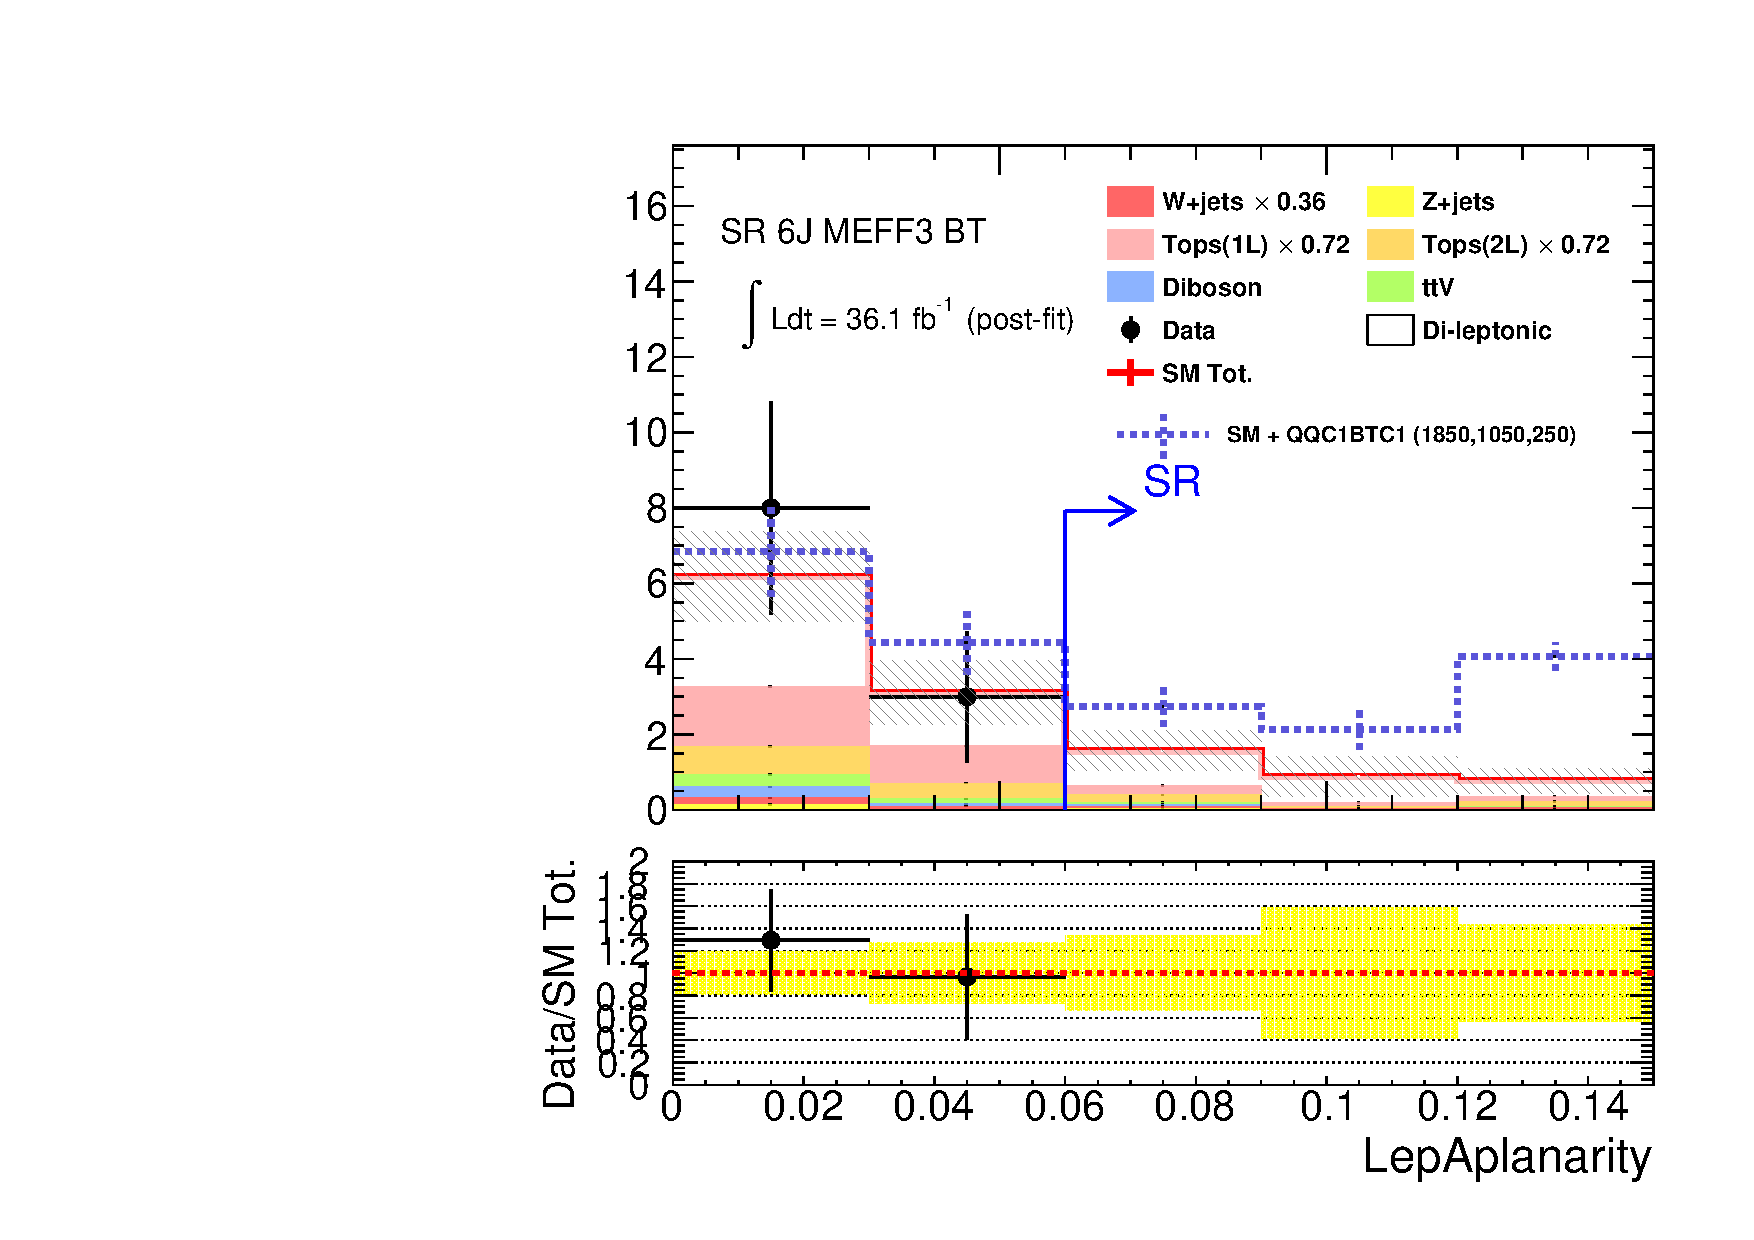
\includegraphics[width=0.41\textwidth]{figures/BGestimation/SRVRpostFit/LepAplanarity__SR6JMEFF3BT_no_LepAplanarity_postFit_2SFconfig_noYields_objRep.pdf}}
    \caption{
      Post-fit distruibution of (left) $\mt$, and (right) $\apl$.
      (a,b) SR 6J-$\meffIncFirst$ BT.
      (c,d) SR 6J-$\meffIncSecond$ BT.
      (e,f) SR 6J-$\meffIncThird$ BT.
      The yellow band in the bottom panel represents only statistical error. The overflow is included in the highest bin.  
      \label{fig::BGestimation::SRVRpostFit::SR6JBT}
    }
\end{figure}

\clearpage
\begin{figure}[h]
  \centering
    \subfigure[]{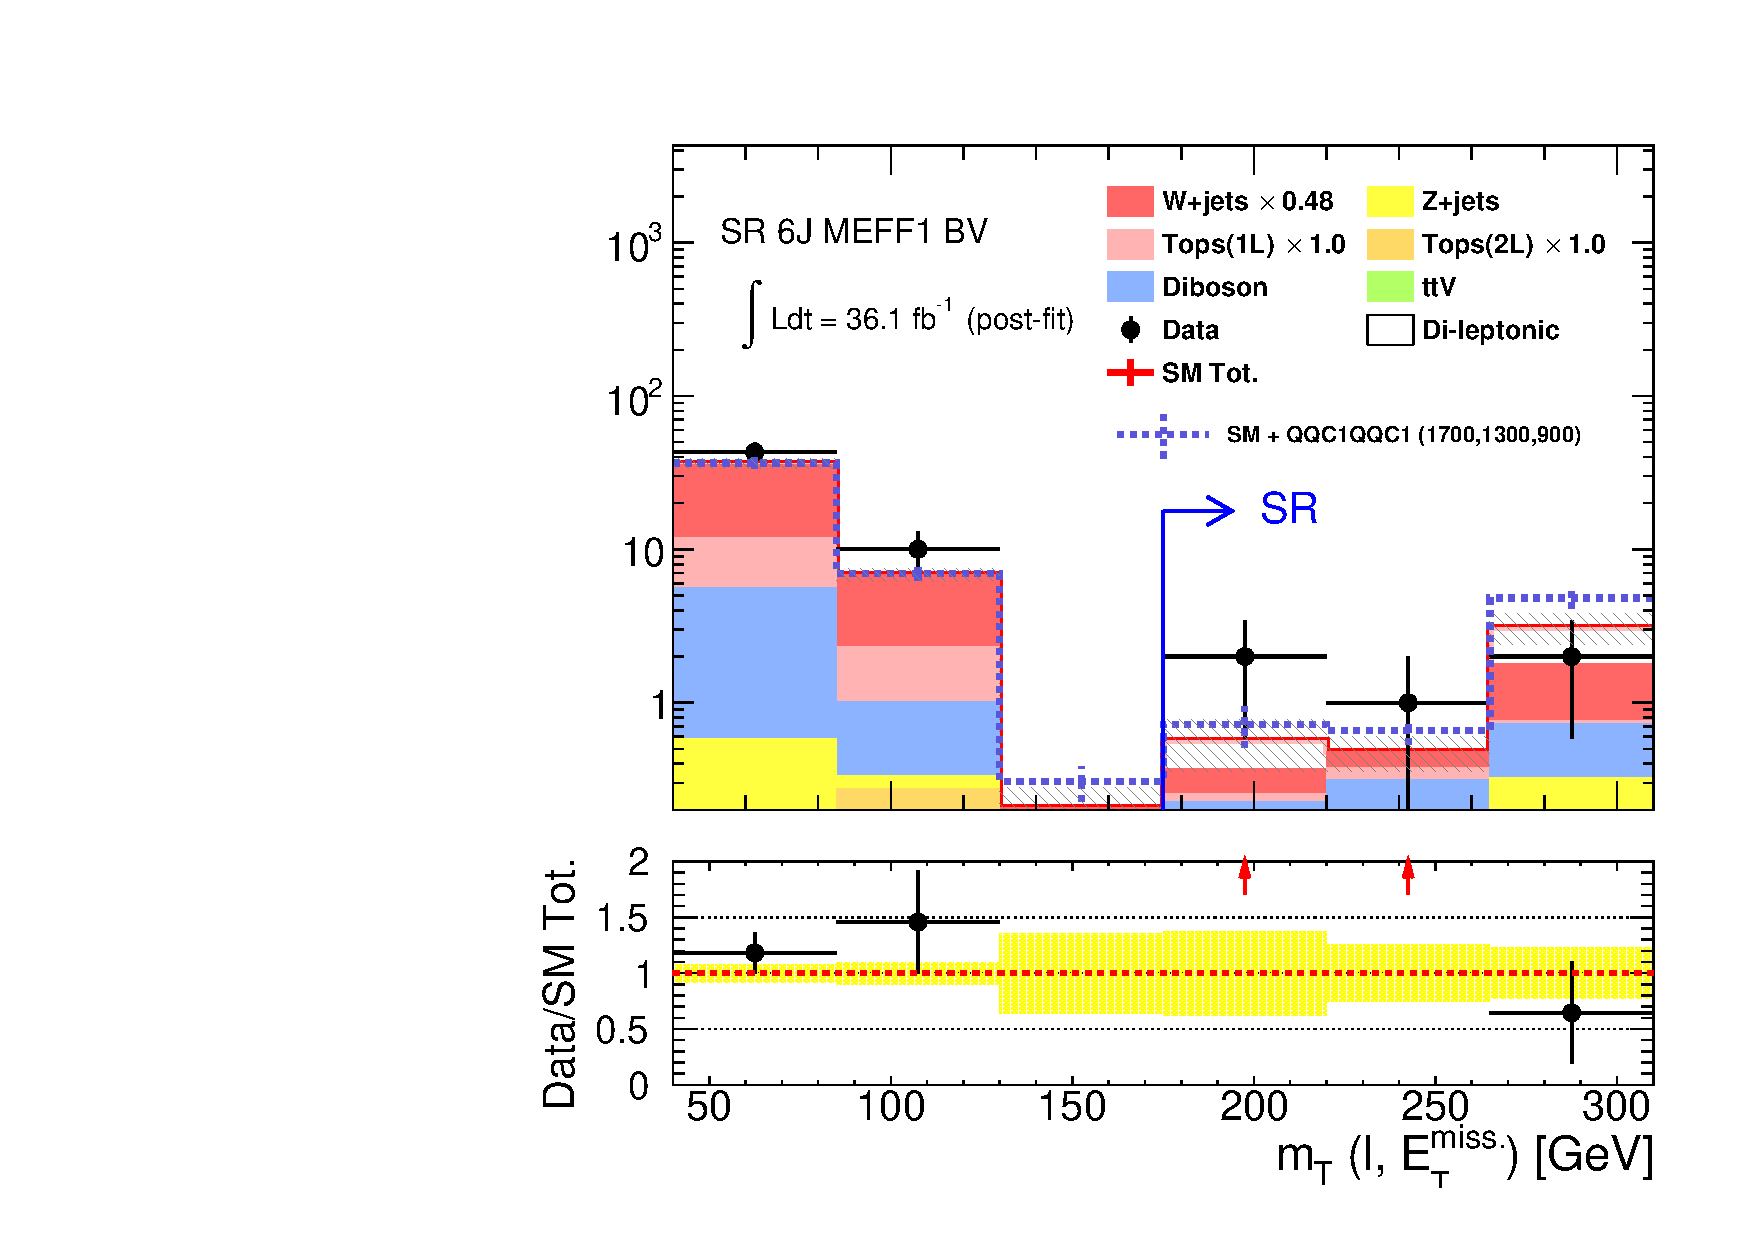
\includegraphics[width=0.41\textwidth]{figures/BGestimation/SRVRpostFit/mt__SR6JMEFF1BV_no_mt_postFit_2SFconfig_noYields_objRep.pdf}}
    \subfigure[]{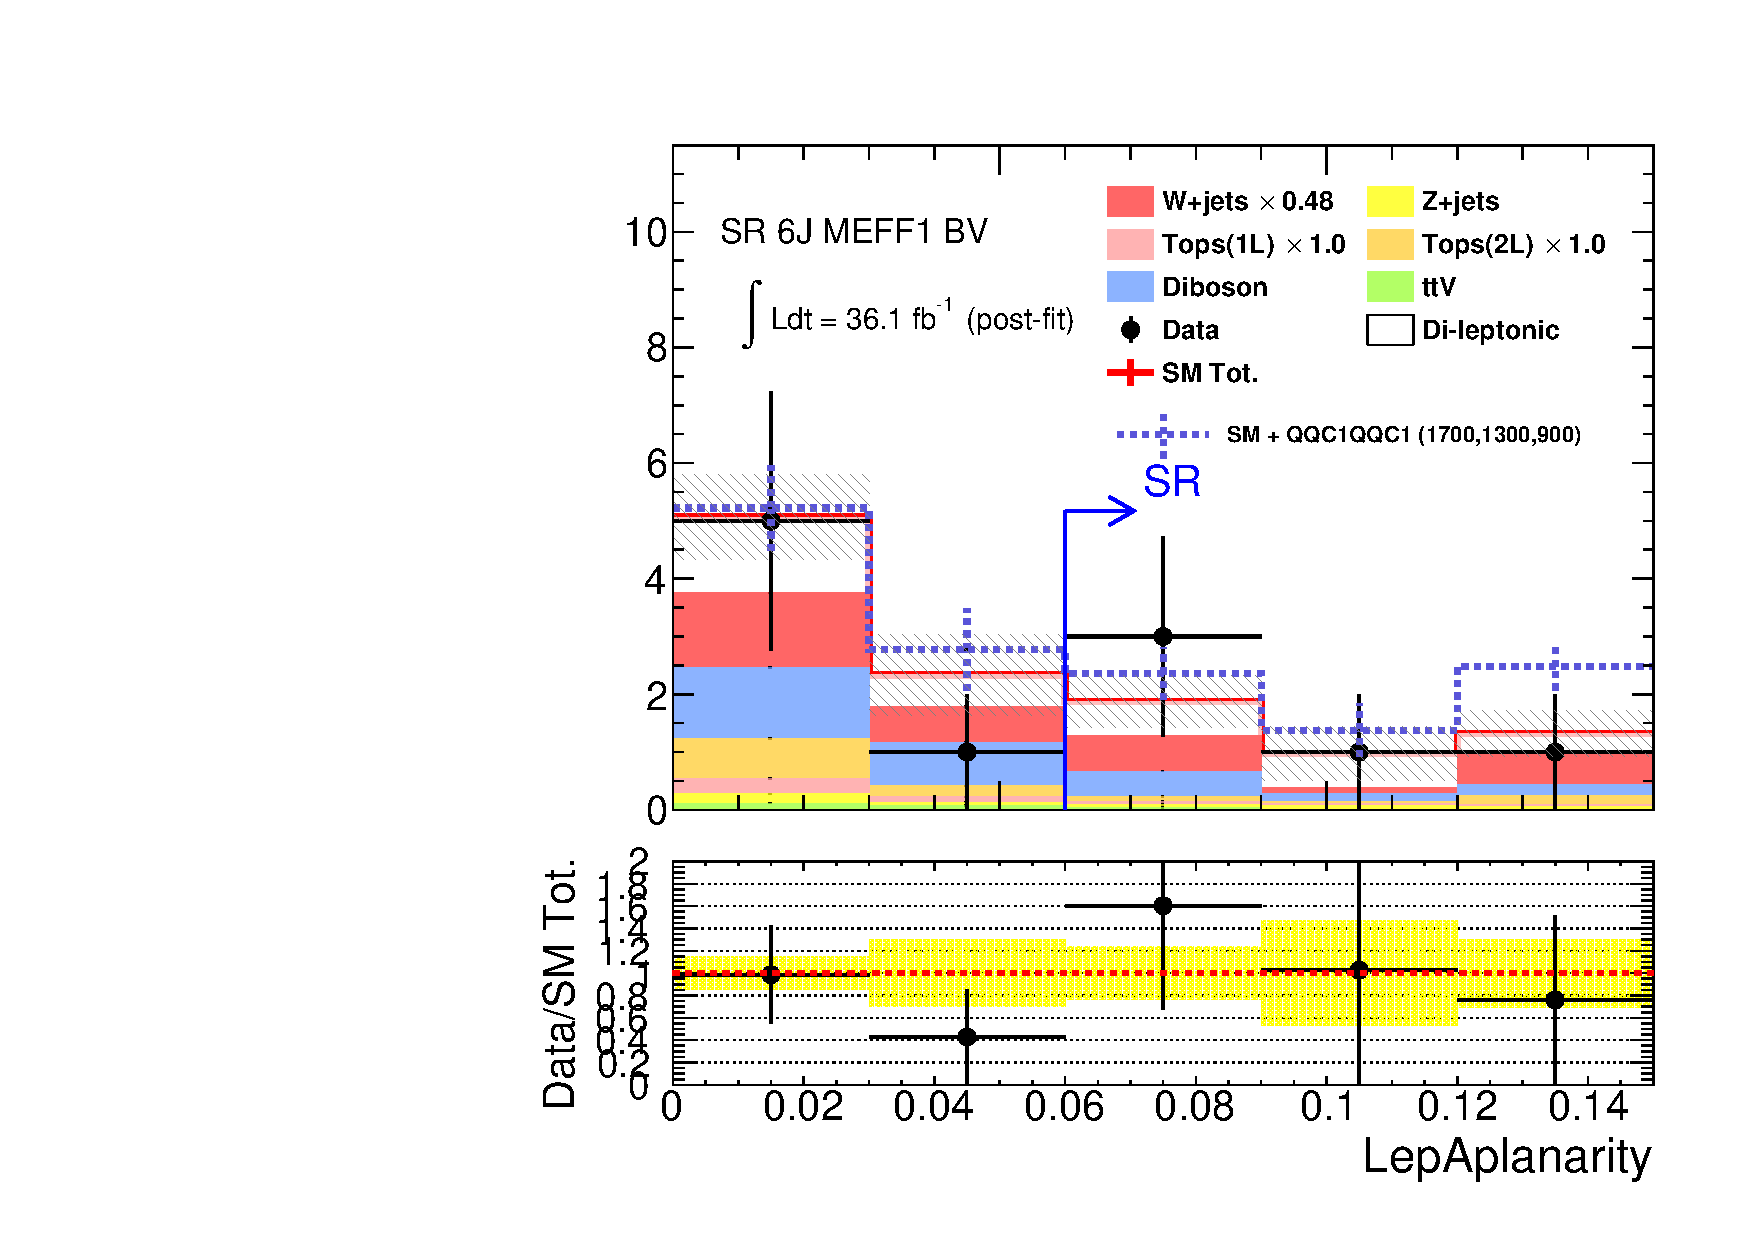
\includegraphics[width=0.41\textwidth]{figures/BGestimation/SRVRpostFit/LepAplanarity__SR6JMEFF1BV_no_LepAplanarity_postFit_2SFconfig_noYields_objRep.pdf}}
    \subfigure[]{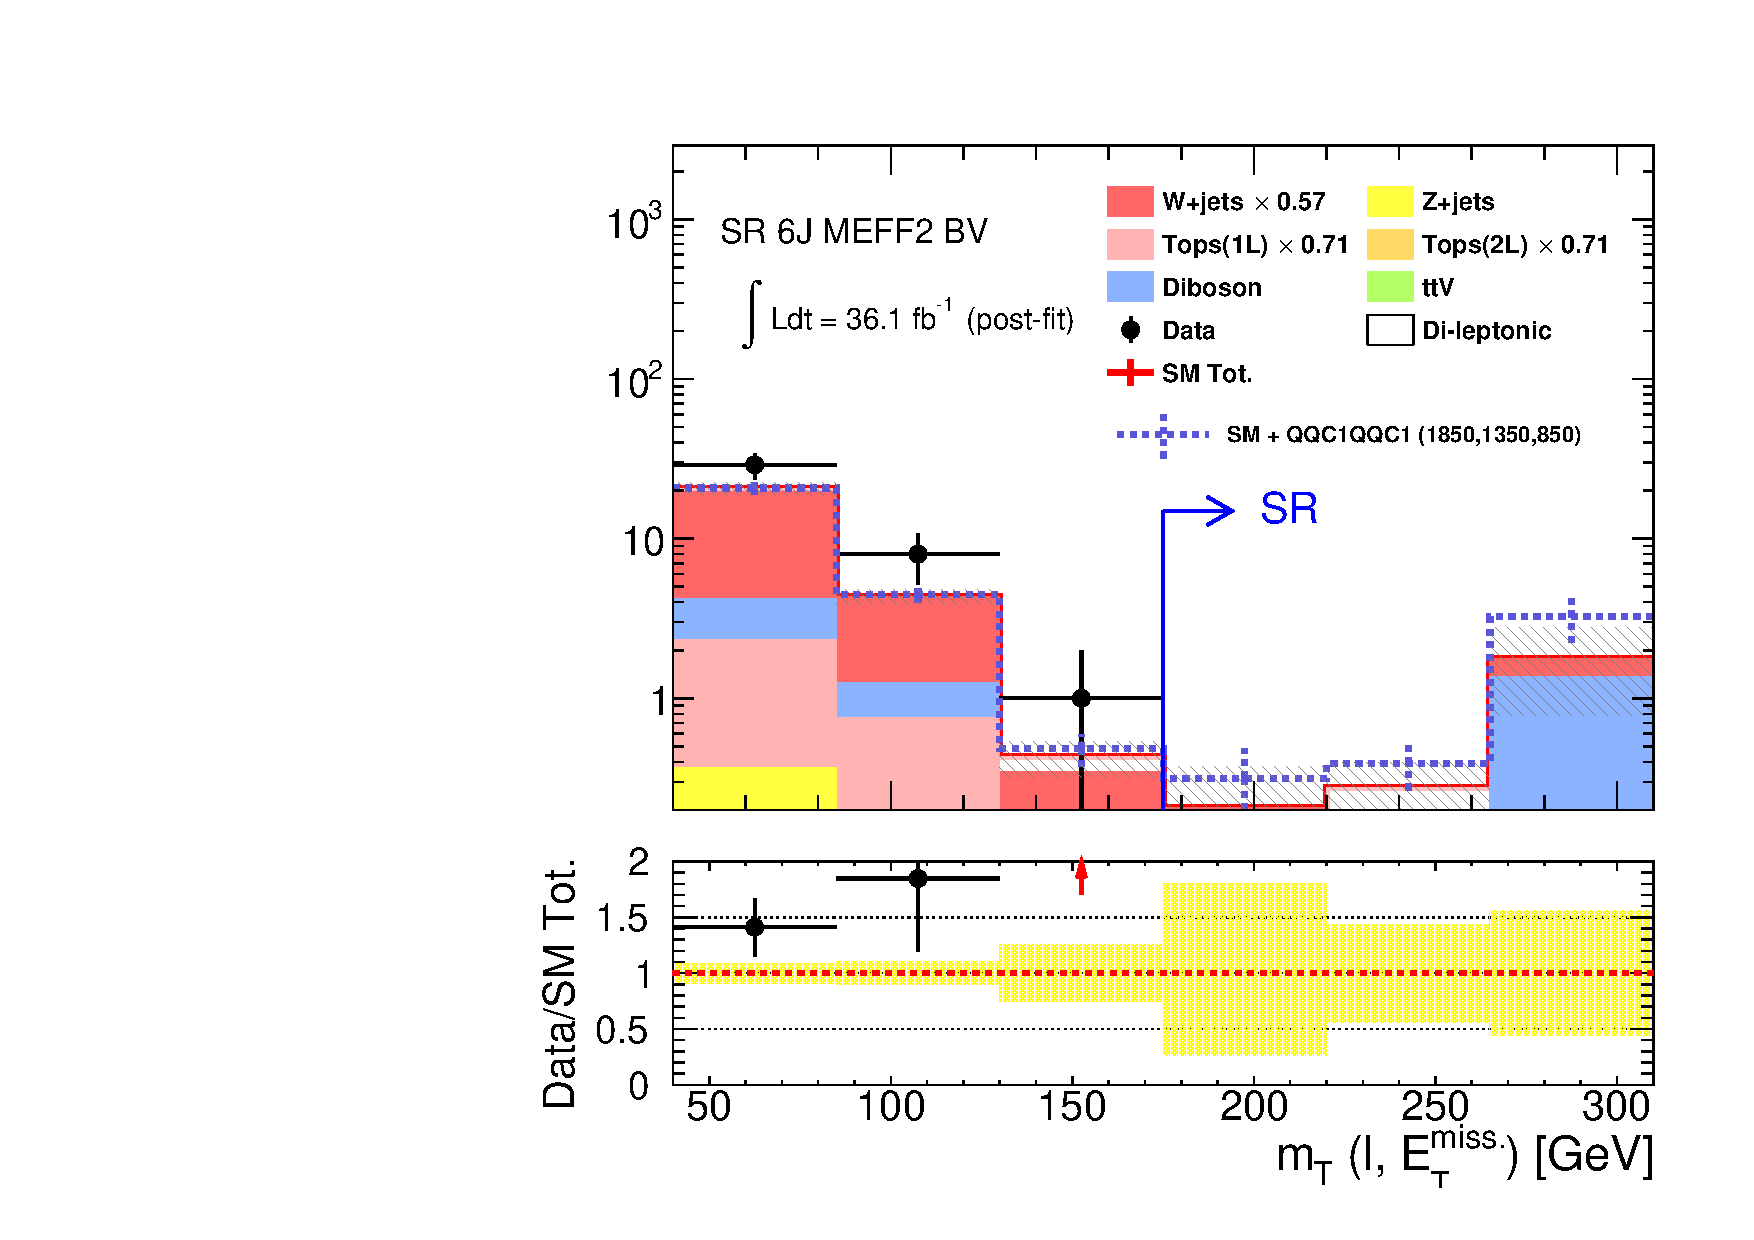
\includegraphics[width=0.41\textwidth]{figures/BGestimation/SRVRpostFit/mt__SR6JMEFF2BV_no_mt_postFit_2SFconfig_noYields_objRep.pdf}}
    \subfigure[]{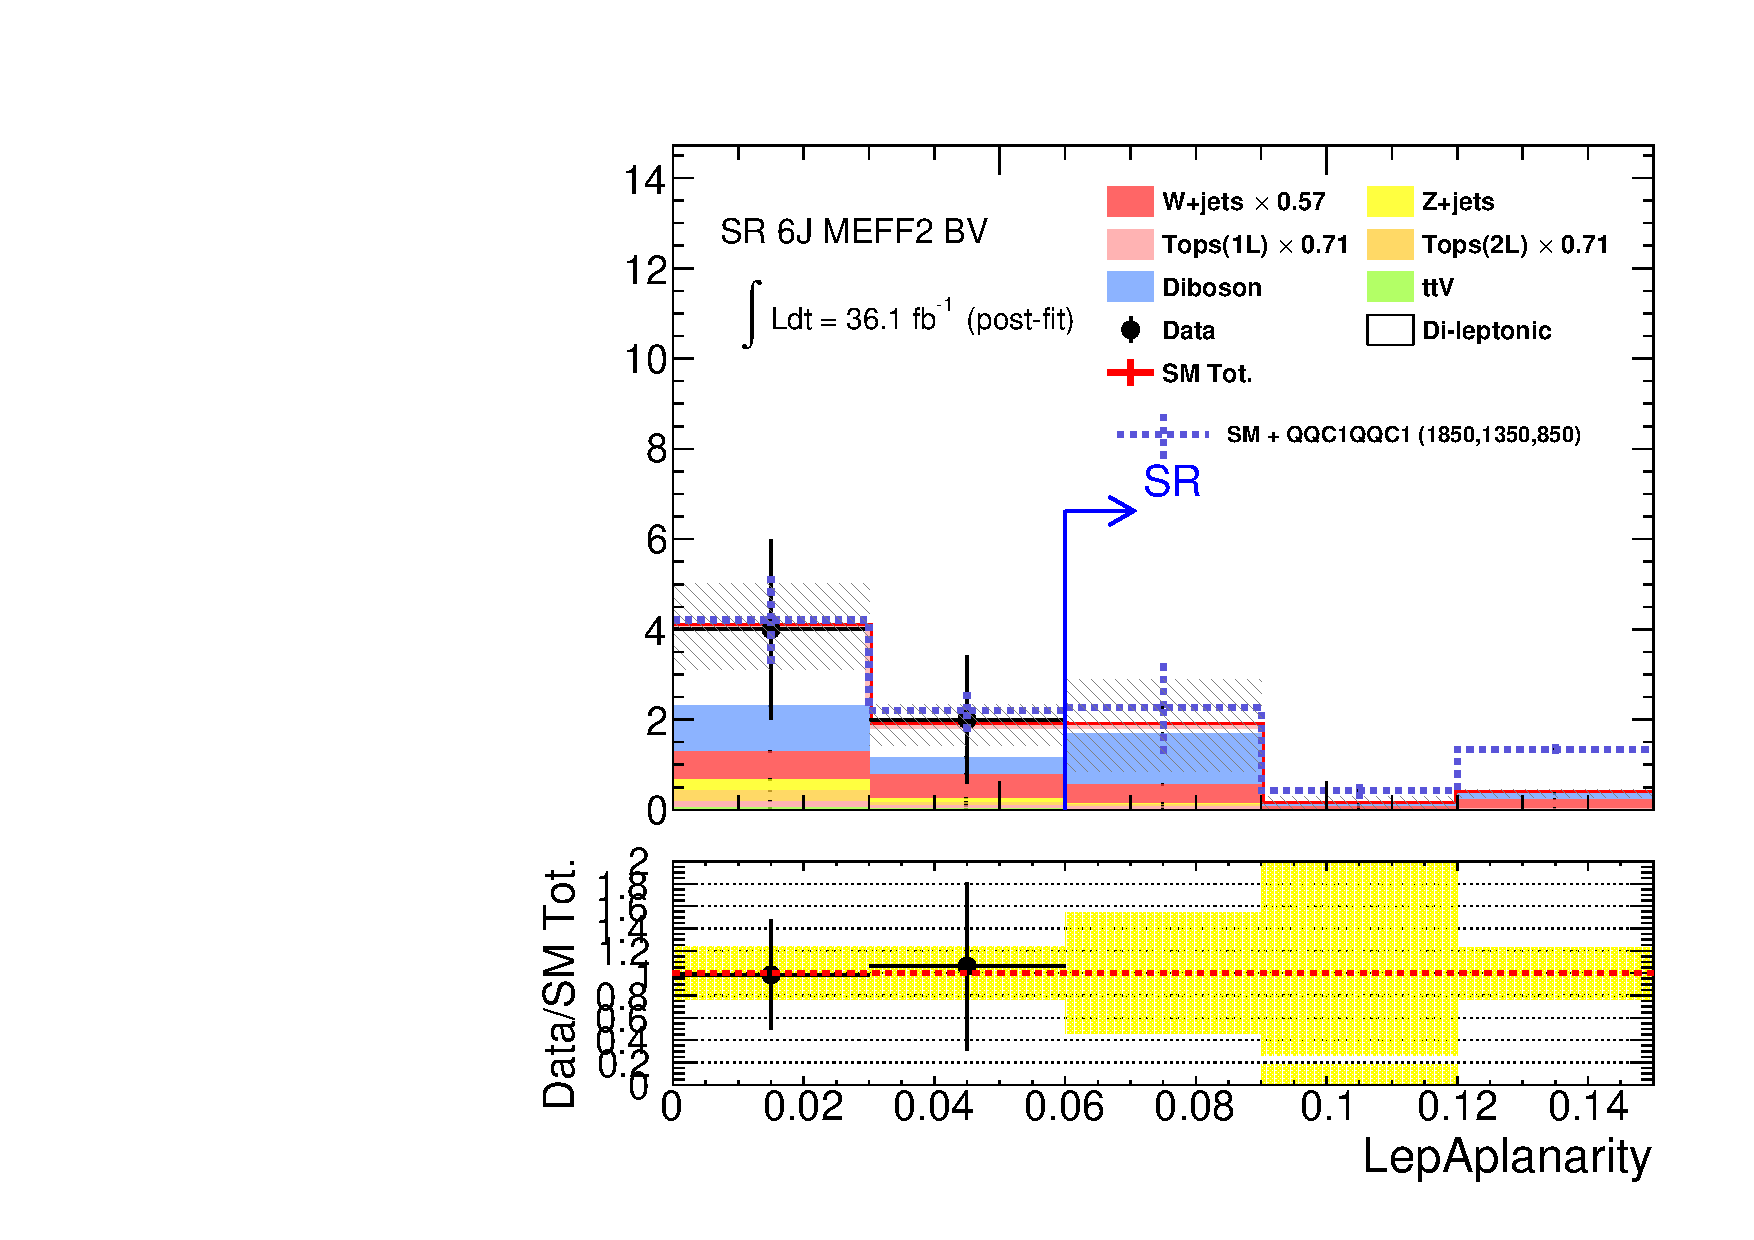
\includegraphics[width=0.41\textwidth]{figures/BGestimation/SRVRpostFit/LepAplanarity__SR6JMEFF2BV_no_LepAplanarity_postFit_2SFconfig_noYields_objRep.pdf}}
    \subfigure[]{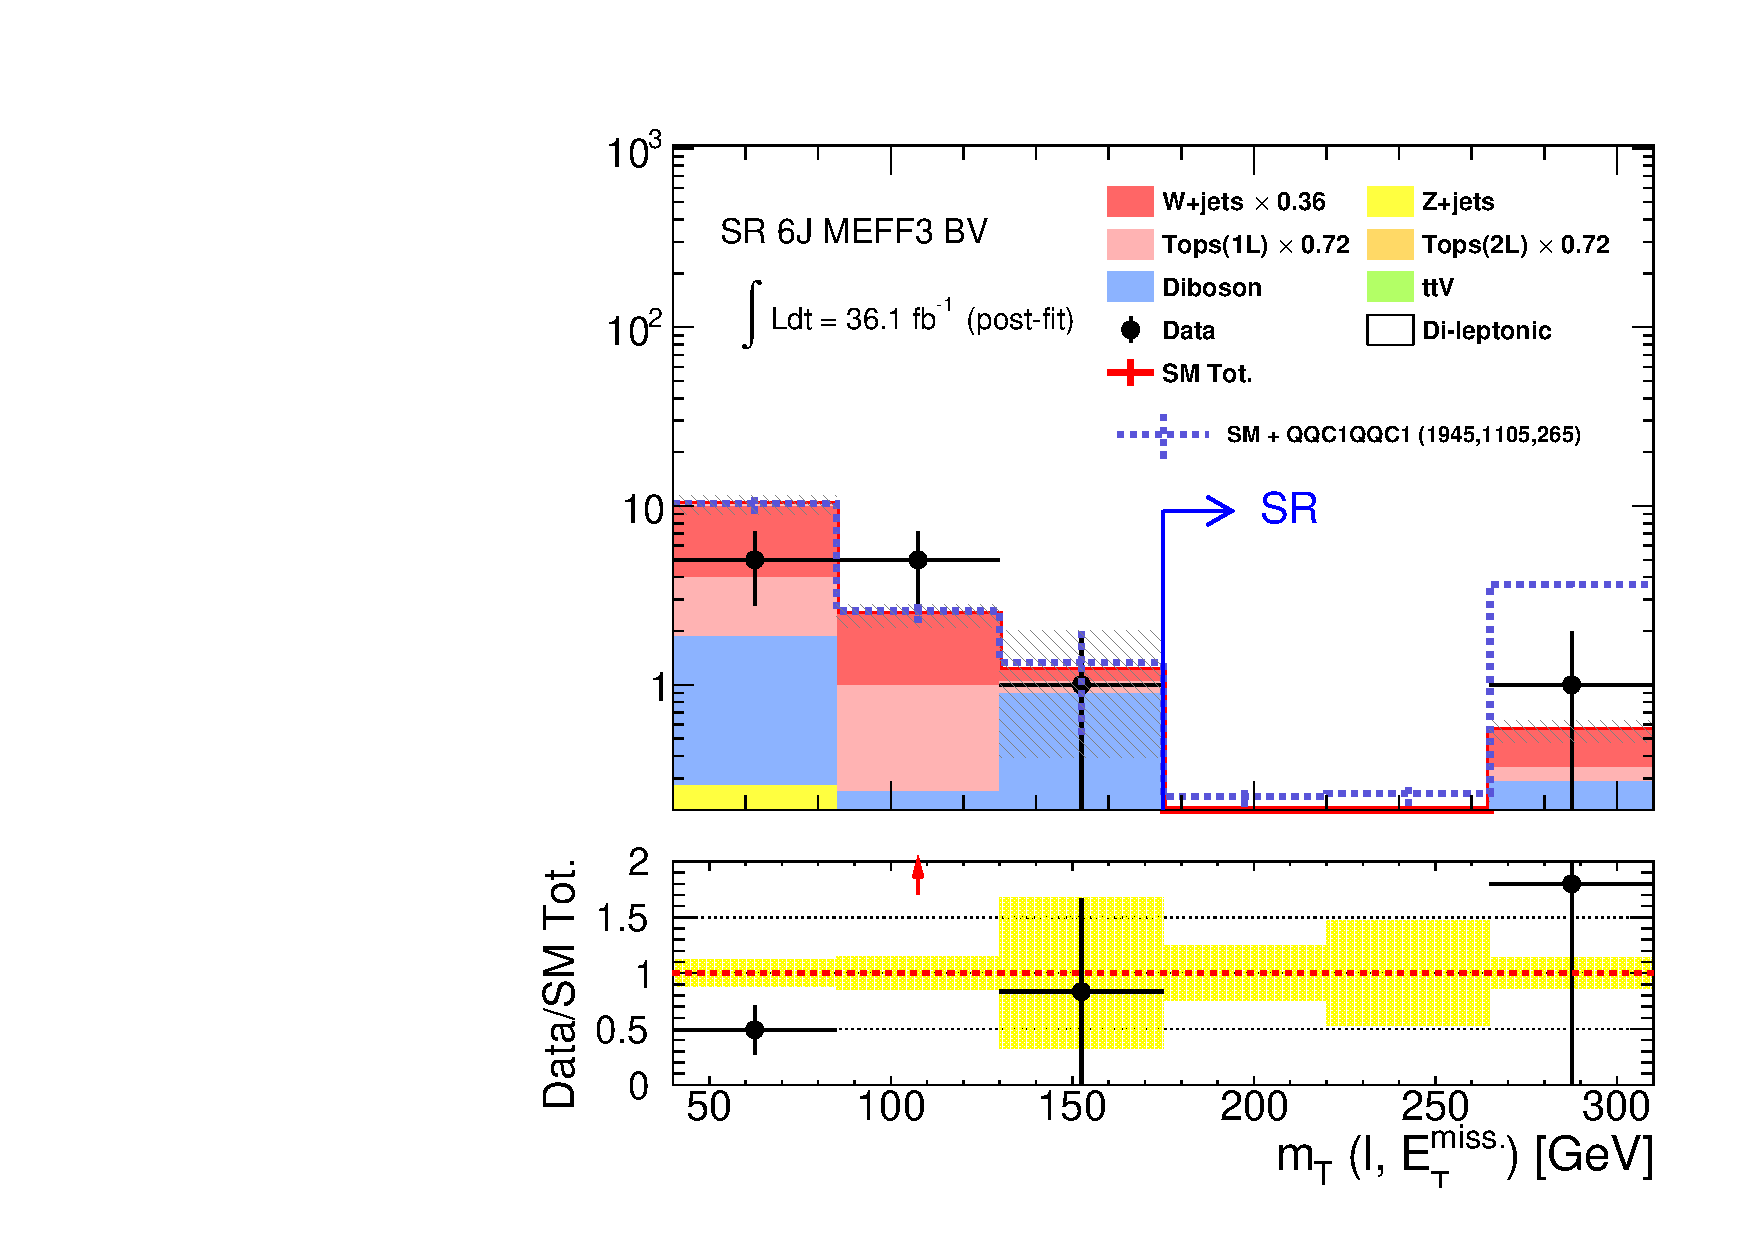
\includegraphics[width=0.41\textwidth]{figures/BGestimation/SRVRpostFit/mt__SR6JMEFF3BV_no_mt_postFit_2SFconfig_noYields_objRep.pdf}}
    \subfigure[]{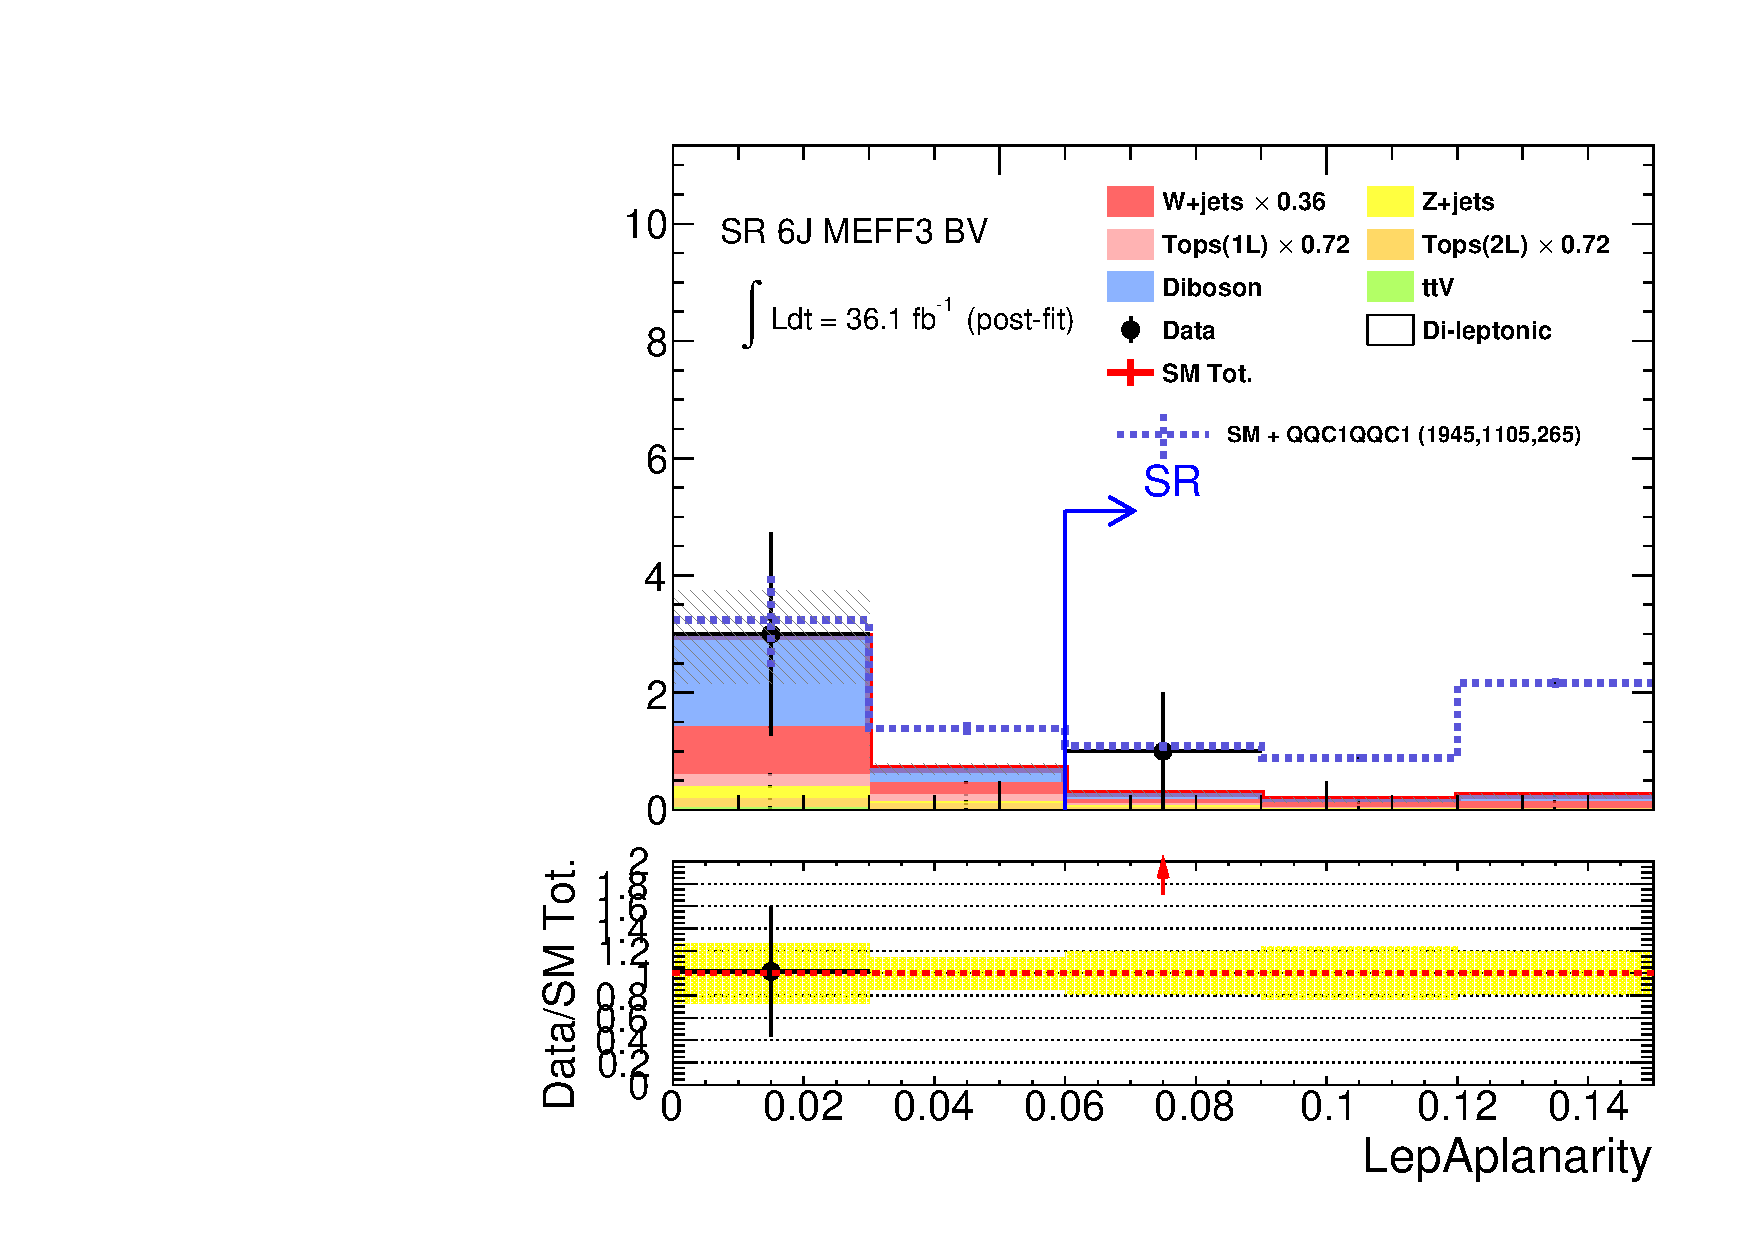
\includegraphics[width=0.41\textwidth]{figures/BGestimation/SRVRpostFit/LepAplanarity__SR6JMEFF3BV_no_LepAplanarity_postFit_2SFconfig_noYields_objRep.pdf}}
    \caption{
      Post-fit distruibution of (left) $\mt$, and (right) $\apl$.
      (a,b) SR 6J-$\meffIncFirst$ BV.
      (c,d) SR 6J-$\meffIncSecond$ BV.
      (e,f) SR 6J-$\meffIncThird$ BV.
      The yellow band in the bottom panel represents only statistical error. The overflow is included in the highest bin.  
      \label{fig::BGestimation::SRVRpostFit::SR6JBV}
    }
\end{figure}
%----------------------------------


\clearpage
% -------------- varx ---------
\begin{figure}[h]
  \centering
    \subfigure[]{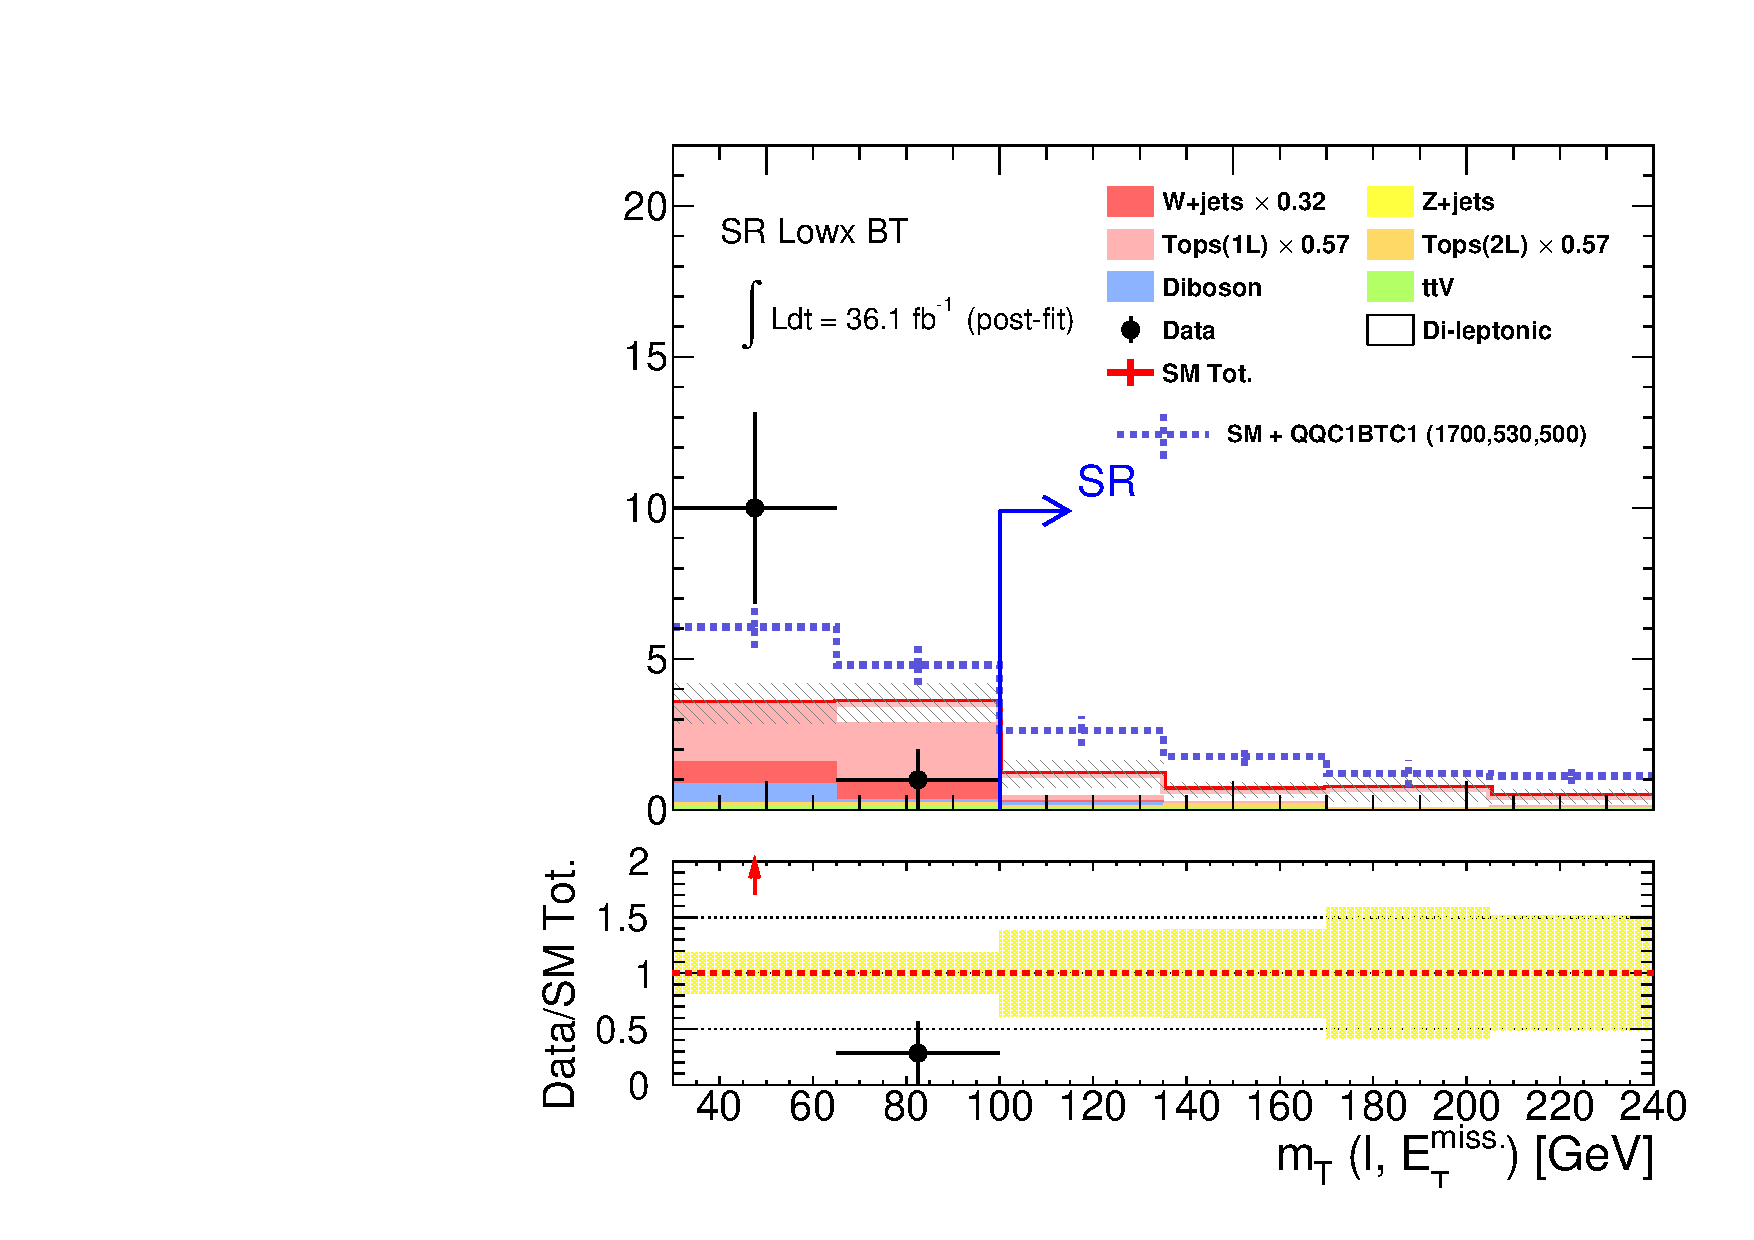
\includegraphics[width=0.41\textwidth]{figures/BGestimation/SRVRpostFit/mt__SRLowxBT_no_mt_postFit_2SFconfig_noYields_objRep.pdf}}
    \subfigure[]{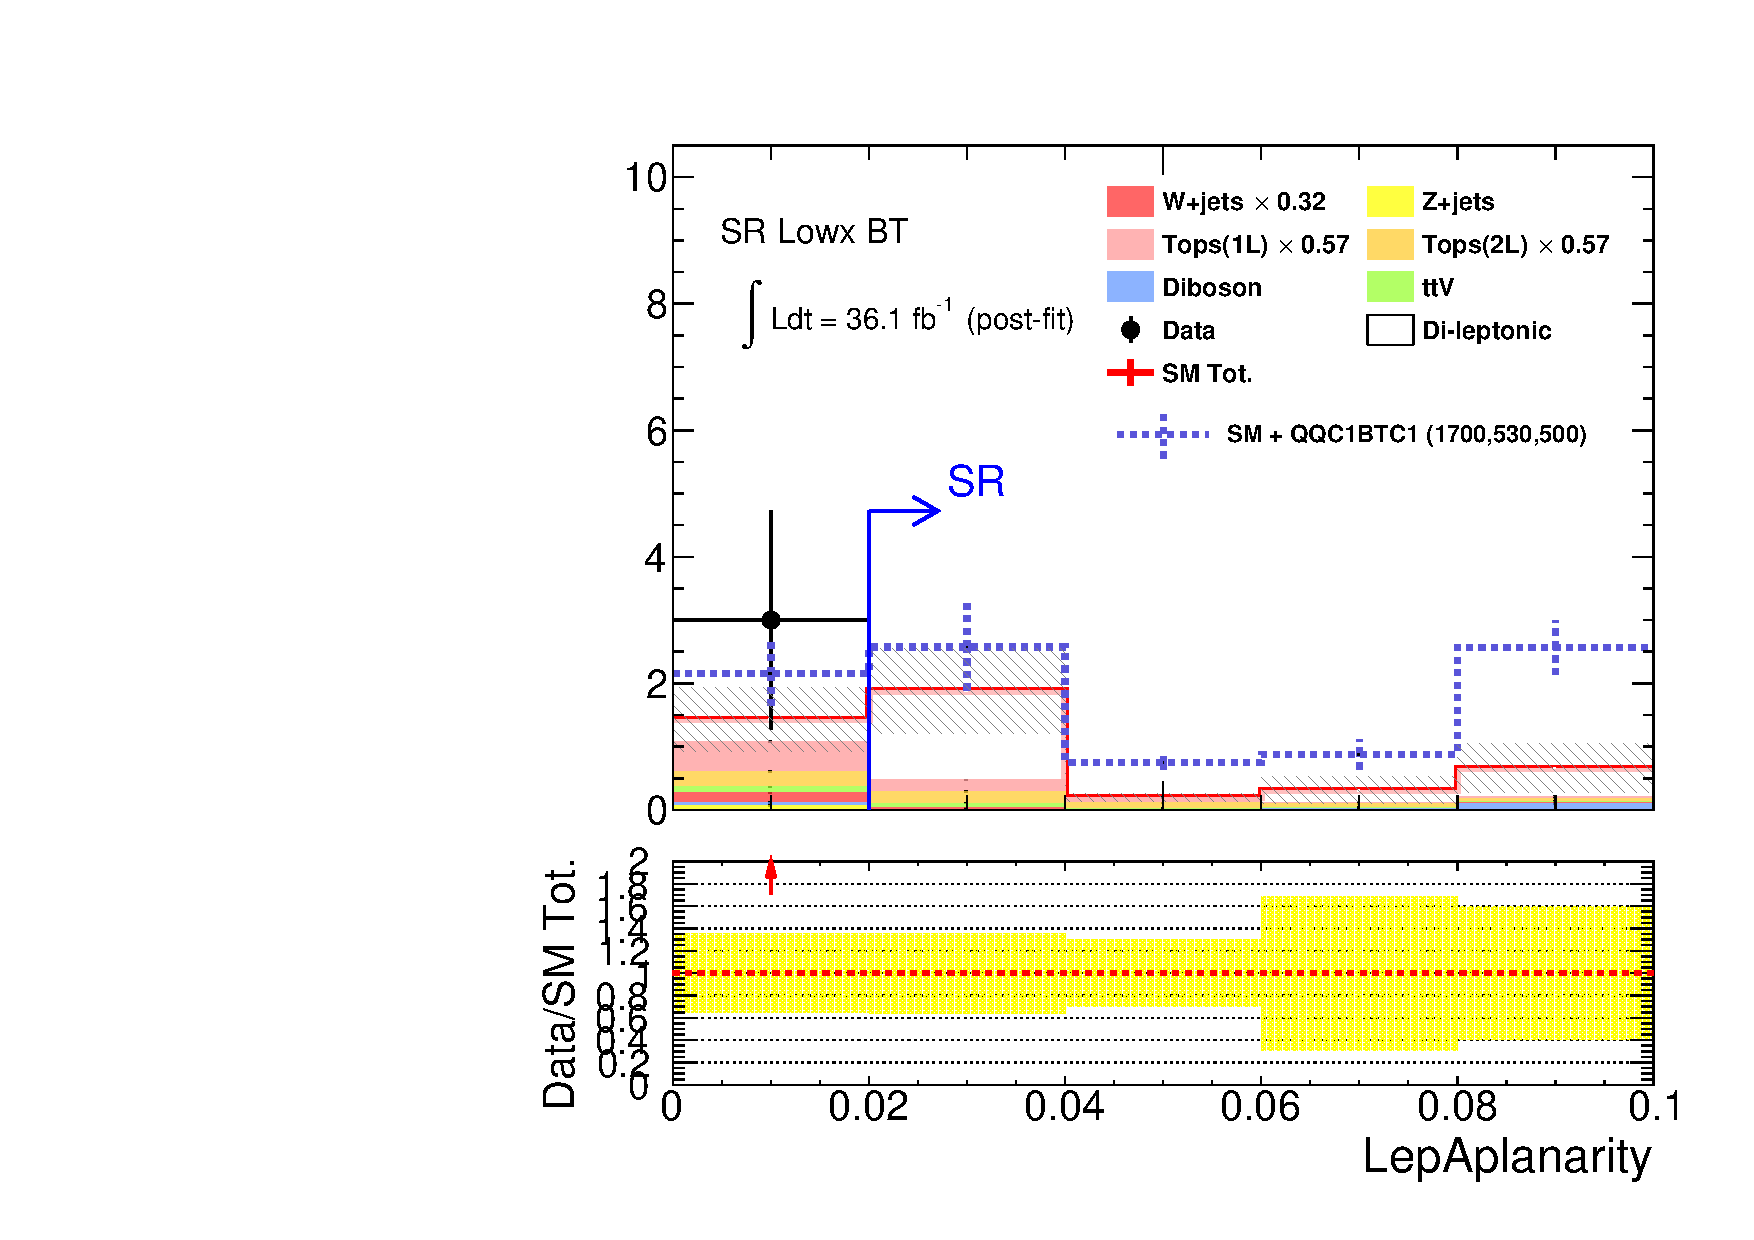
\includegraphics[width=0.41\textwidth]{figures/BGestimation/SRVRpostFit/LepAplanarity__SRLowxBT_no_LepAplanarity_postFit_2SFconfig_noYields_objRep.pdf}}
    \subfigure[]{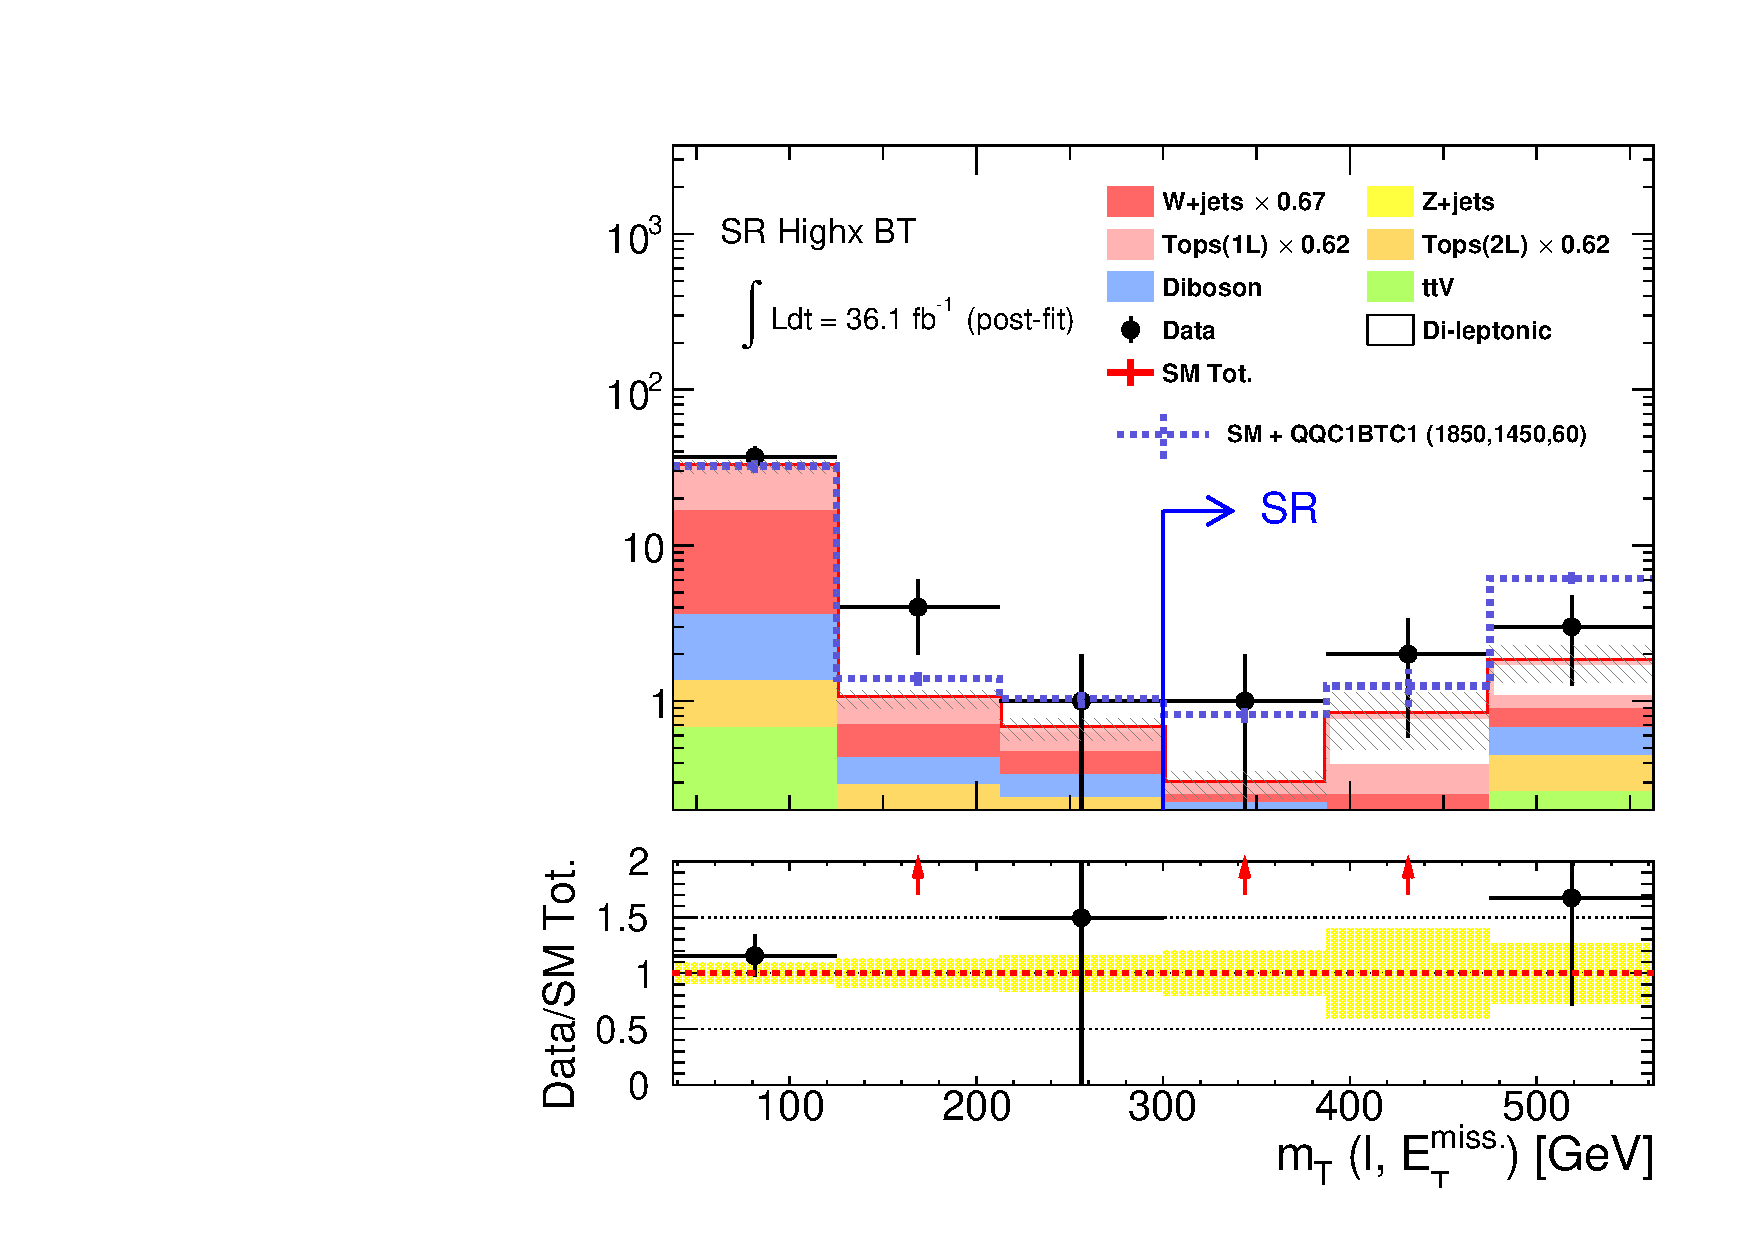
\includegraphics[width=0.41\textwidth]{figures/BGestimation/SRVRpostFit/mt__SRHighxBT_no_mt_postFit_2SFconfig_noYields_objRep.pdf}}
    \subfigure[]{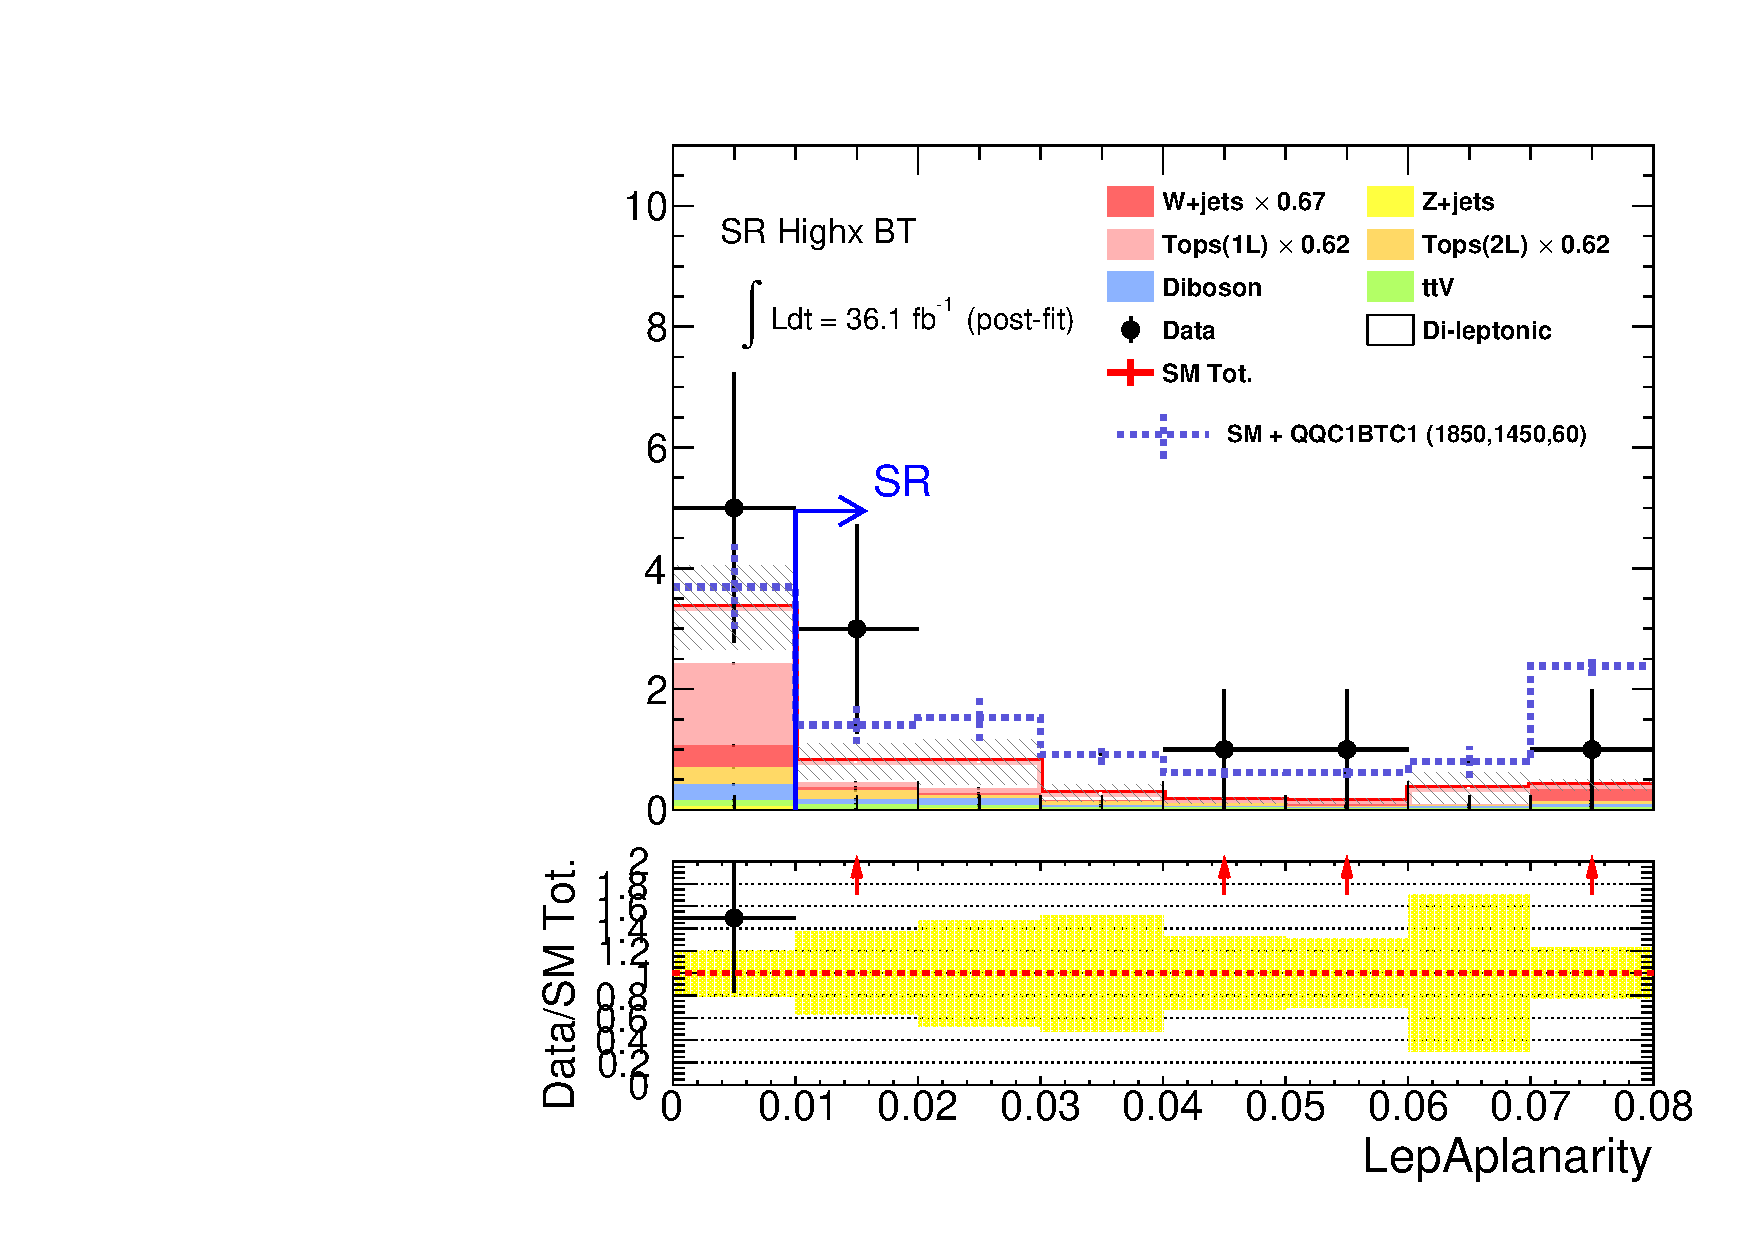
\includegraphics[width=0.41\textwidth]{figures/BGestimation/SRVRpostFit/LepAplanarity__SRHighxBT_no_LepAplanarity_postFit_2SFconfig_noYields_objRep.pdf}}
   \caption{   
     Post-fit distruibution of (left) $\mt$ and (right) $\apl$.
     (a,b) SR Low-x BT.
     (c,d) SR High-x BT.
     The yellow band in the bottom panel represents only statistical error. The overflow is included in the highest bin.  
     \label{fig::BGestimation::SRVRpostFit::SRVarxBT}
   }
\end{figure}

\clearpage
\begin{figure}[h]
  \centering
    \subfigure[]{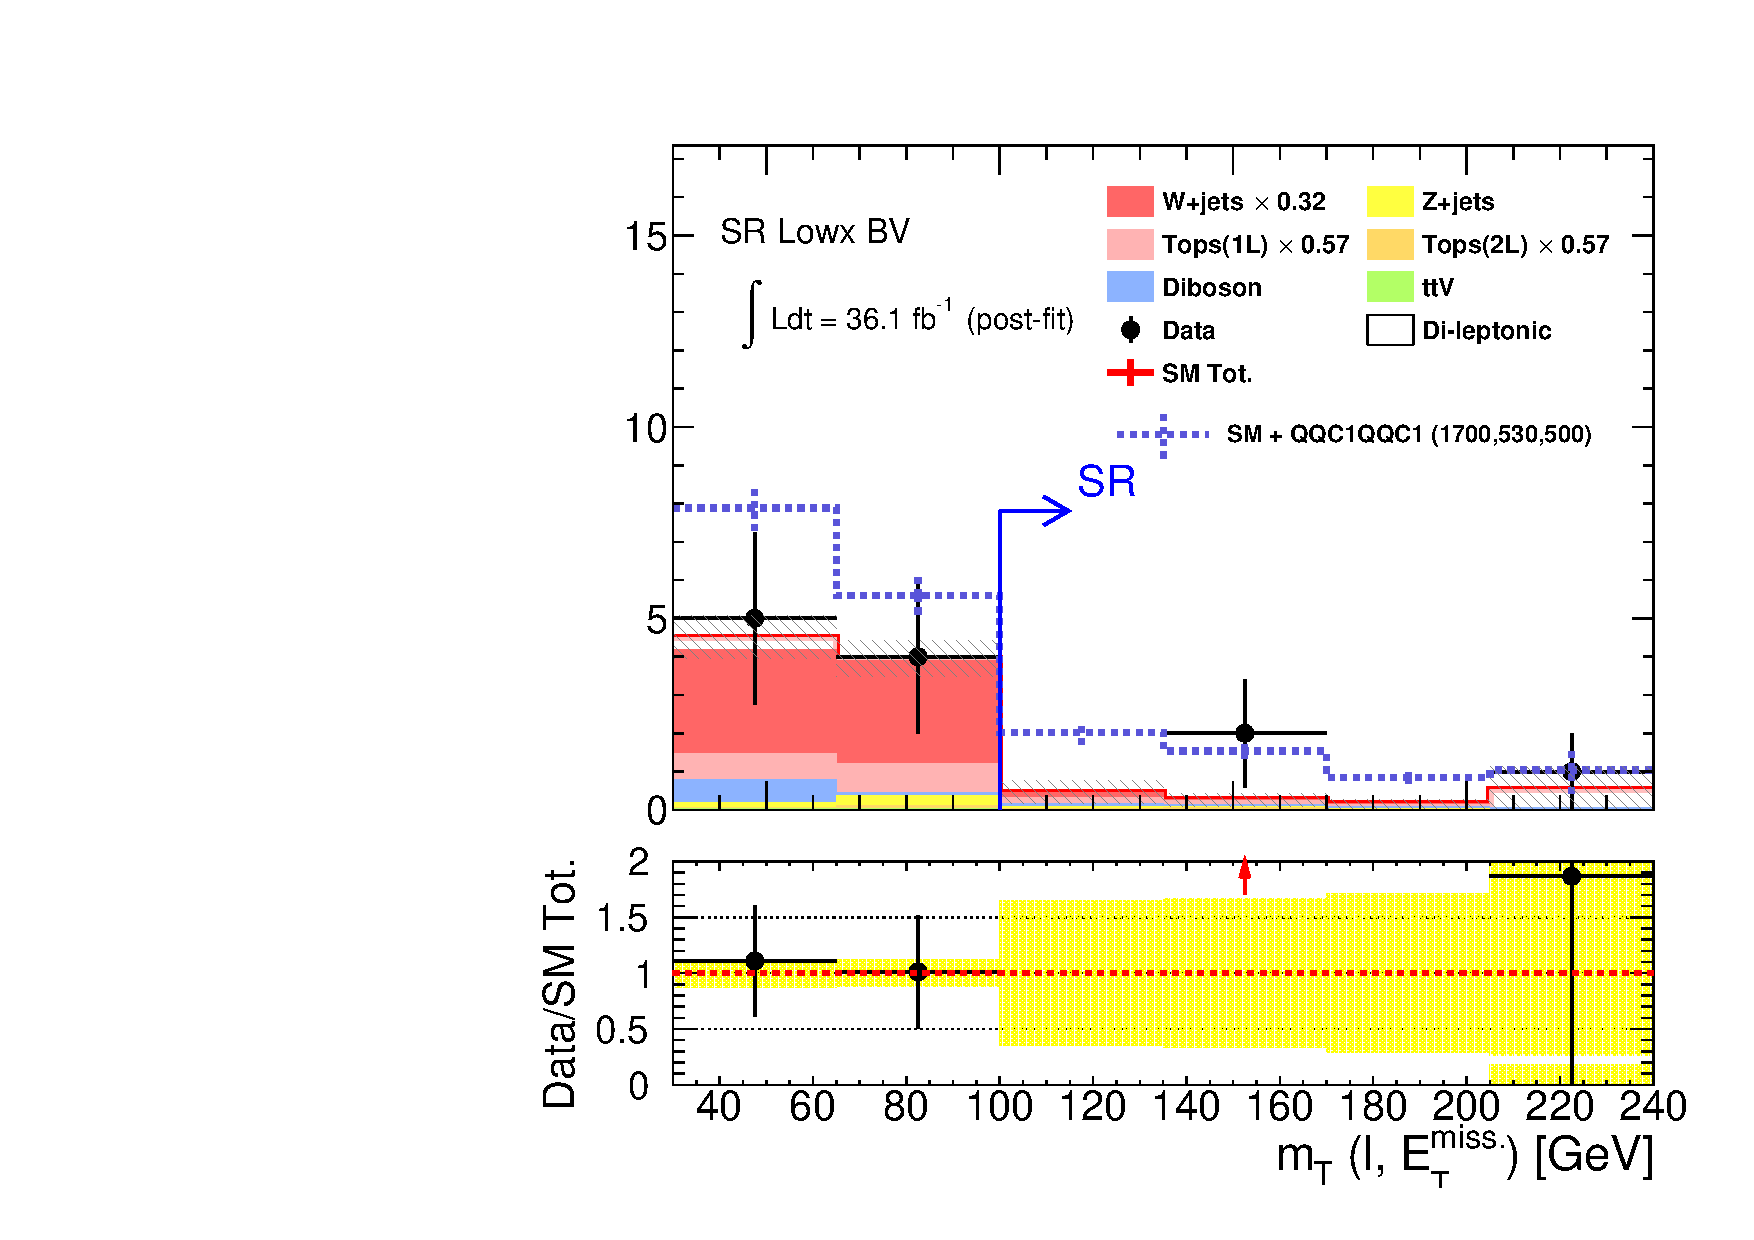
\includegraphics[width=0.41\textwidth]{figures/BGestimation/SRVRpostFit/mt__SRLowxBV_no_mt_postFit_2SFconfig_noYields_objRep.pdf}}
    \subfigure[]{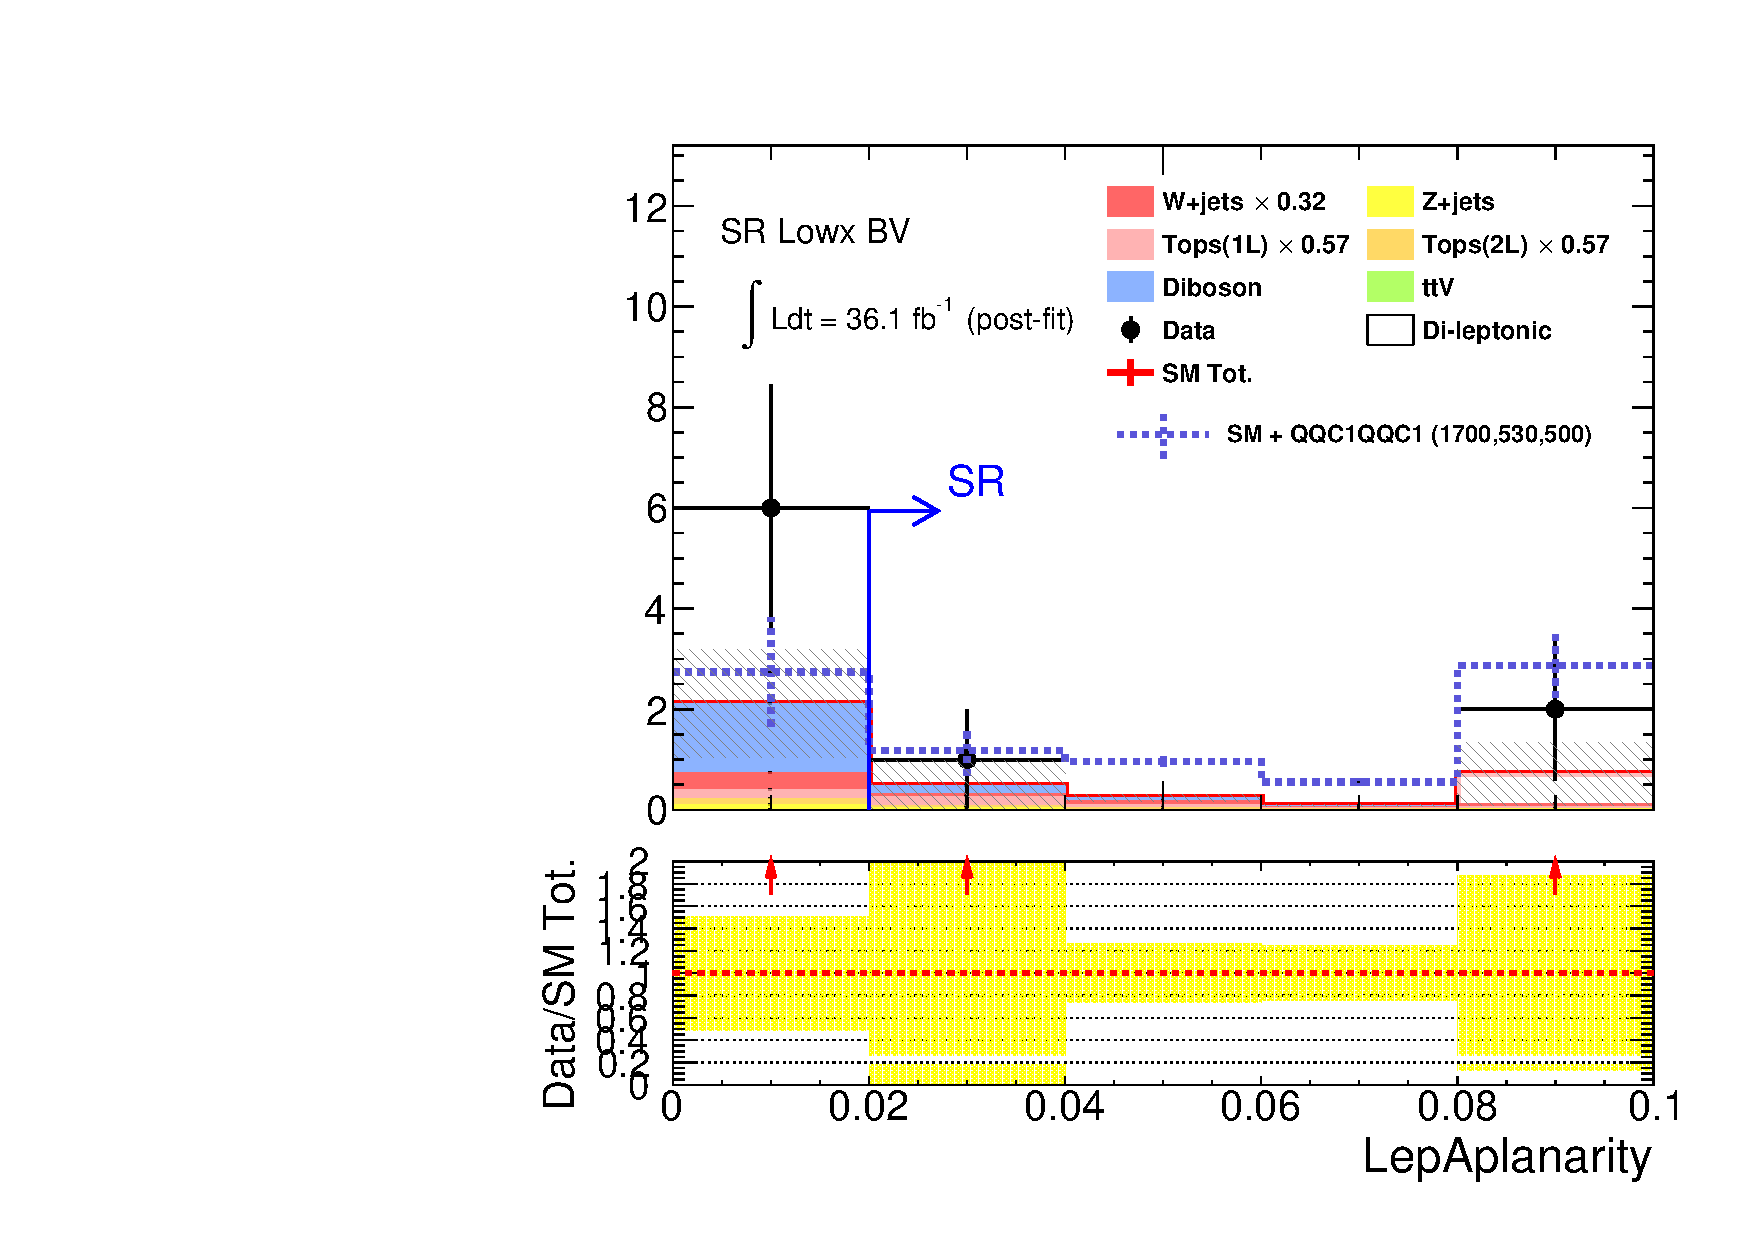
\includegraphics[width=0.41\textwidth]{figures/BGestimation/SRVRpostFit/LepAplanarity__SRLowxBV_no_LepAplanarity_postFit_2SFconfig_noYields_objRep.pdf}}
    \subfigure[]{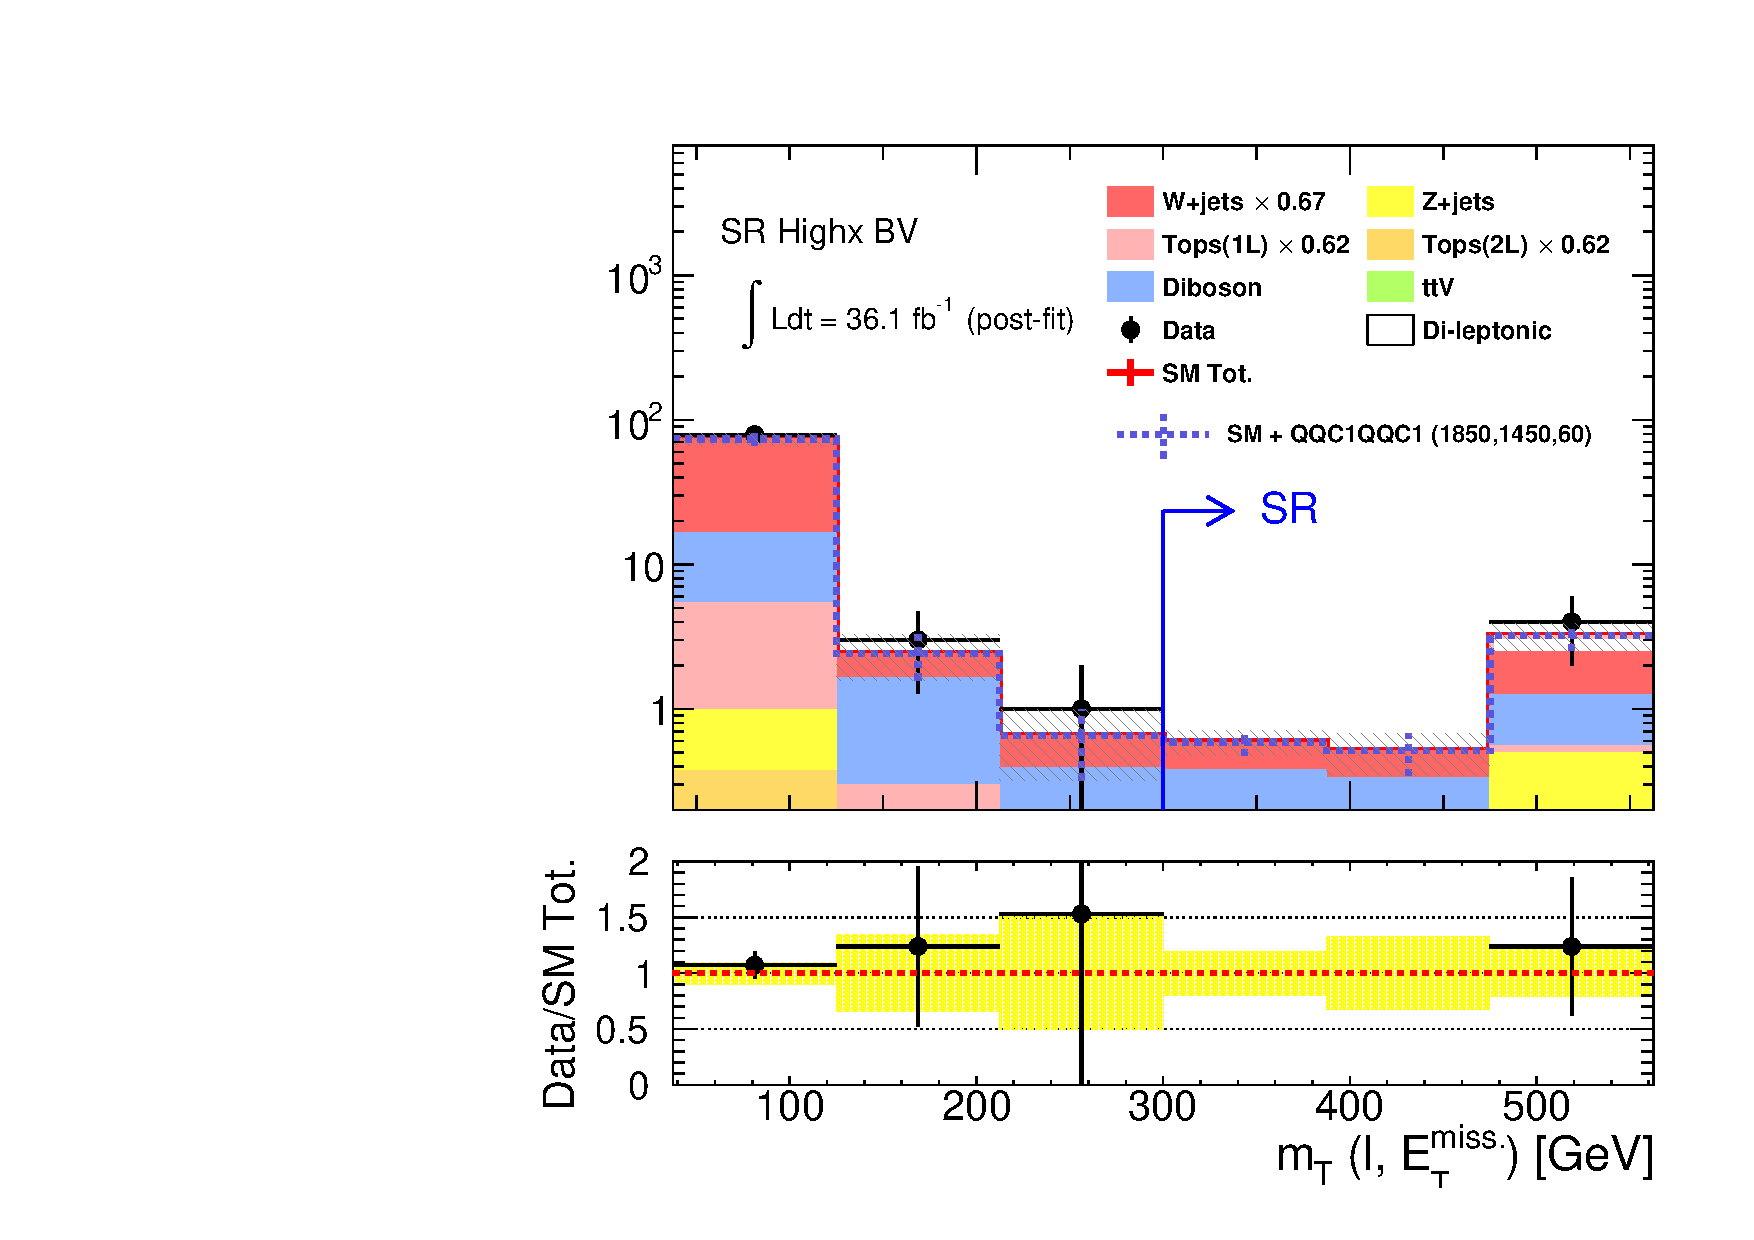
\includegraphics[width=0.41\textwidth]{figures/BGestimation/SRVRpostFit/mt__SRHighxBV_no_mt_postFit_2SFconfig_noYields_objRep.pdf}}
    \subfigure[]{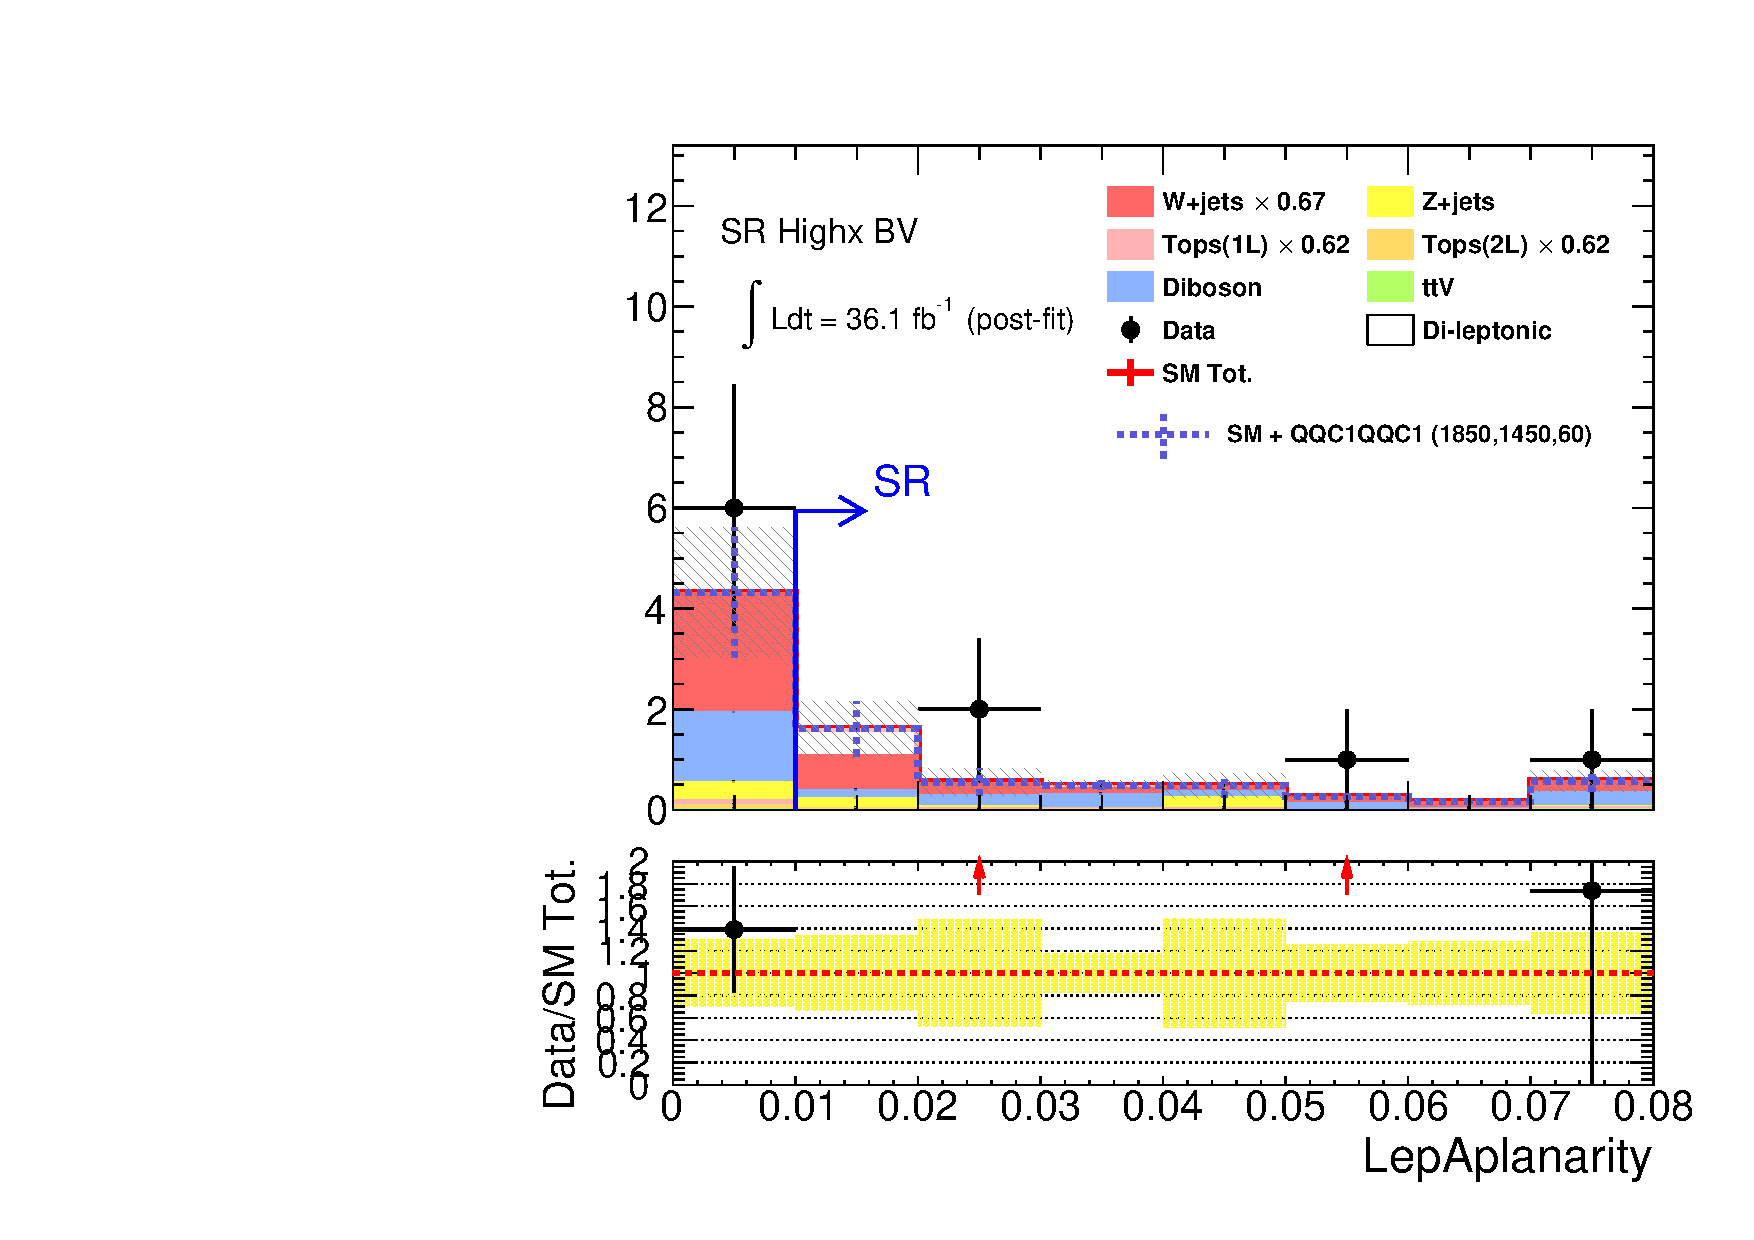
\includegraphics[width=0.41\textwidth]{figures/BGestimation/SRVRpostFit/LepAplanarity__SRHighxBV_no_LepAplanarity_postFit_2SFconfig_noYields_objRep.pdf}}
   \caption{   
     Post-fit distruibution of (left) $\mt$ and (right) $\apl$.
     (a,b) SR Low-x BV.
     (c,d) SR High-x BV.
     The yellow band in the bottom panel represents only statistical error. The overflow is included in the highest bin.  
     \label{fig::BGestimation::SRVRpostFit::SRVarxBV}
   }
\end{figure}

% ----------------------------------------------

\clearpage
% -------------- 3B ---------
\begin{figure}[h]
  \centering
    \subfigure[]{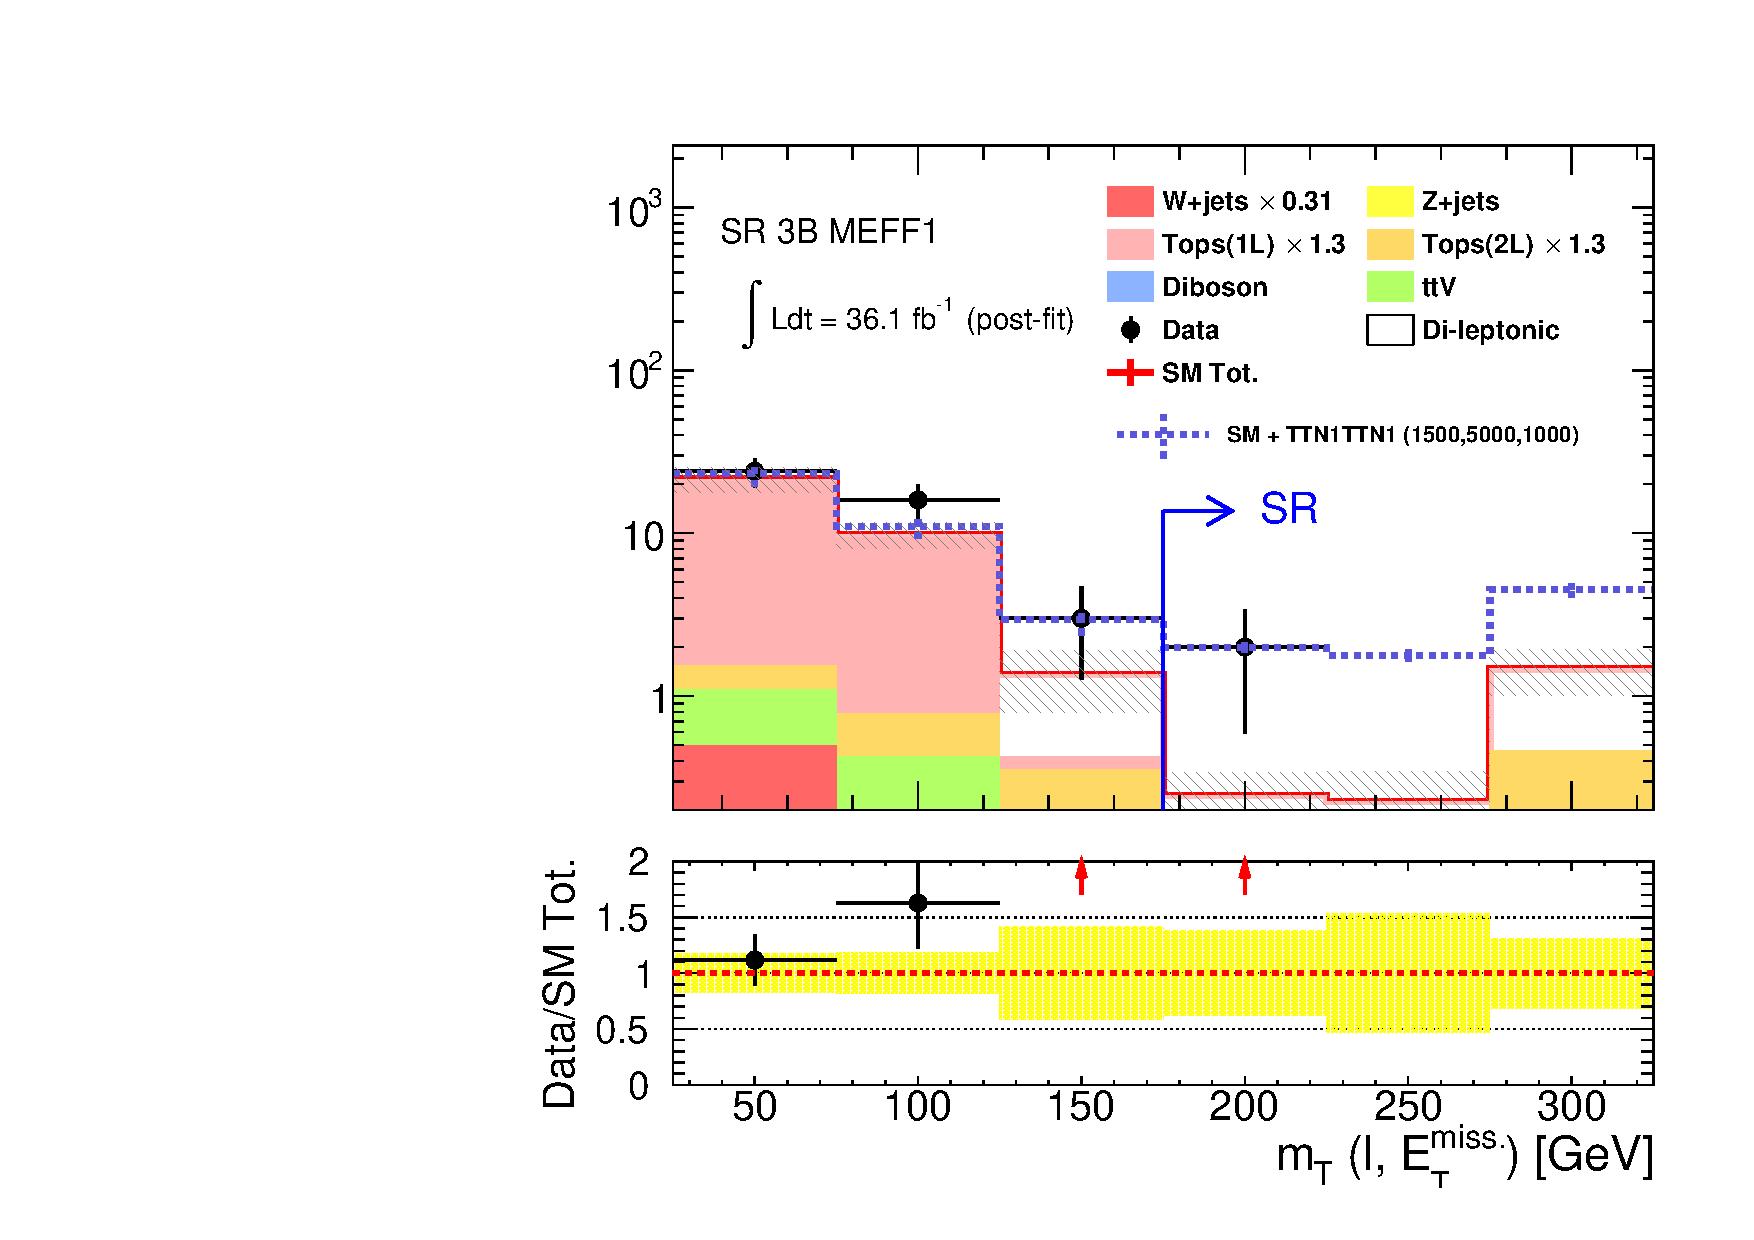
\includegraphics[width=0.41\textwidth]{figures/BGestimation/SRVRpostFit/mt__SR3BMEFF1_no_mt_postFit_2SFconfig_noYields_objRep.pdf}}
    \subfigure[]{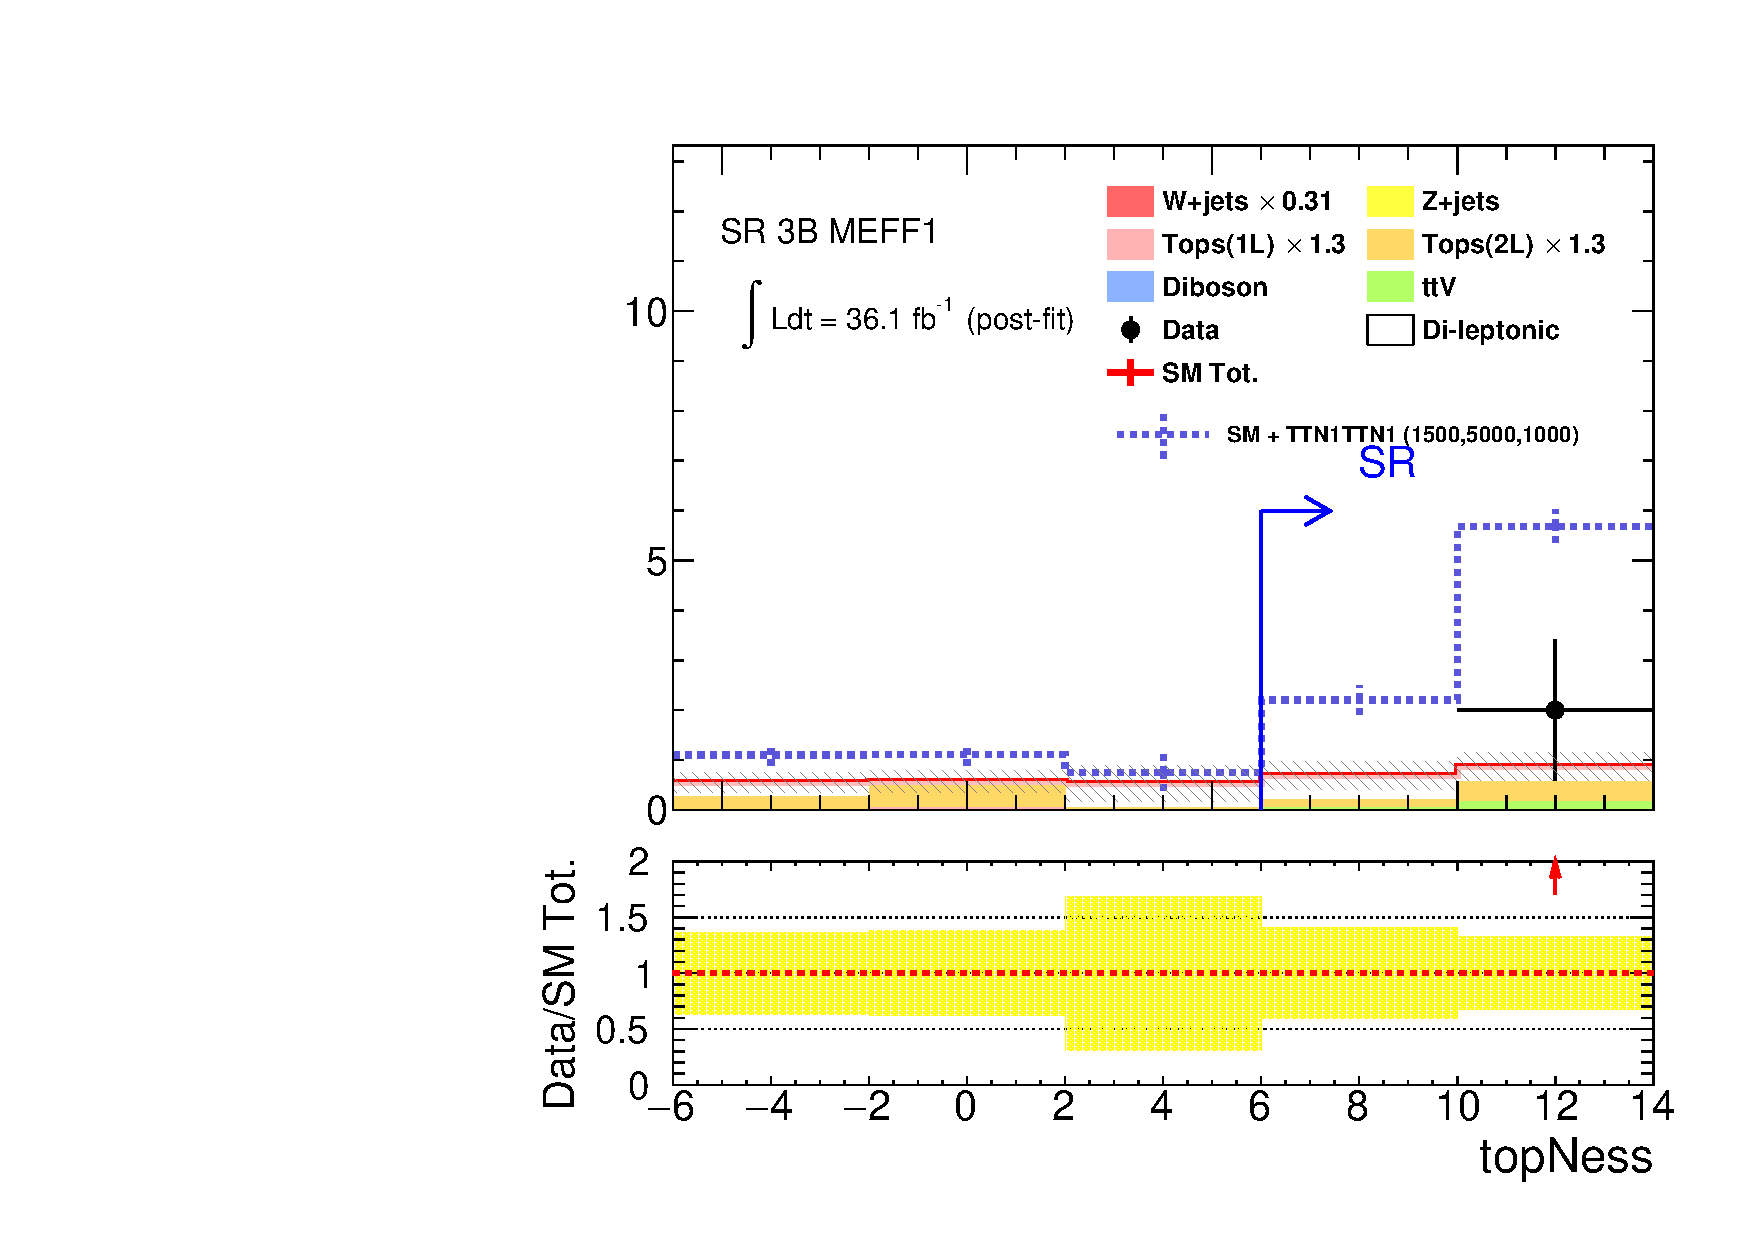
\includegraphics[width=0.41\textwidth]{figures/BGestimation/SRVRpostFit/topNess__SR3BMEFF1_no_topNess_postFit_2SFconfig_noYields_objRep.pdf}}
    \subfigure[]{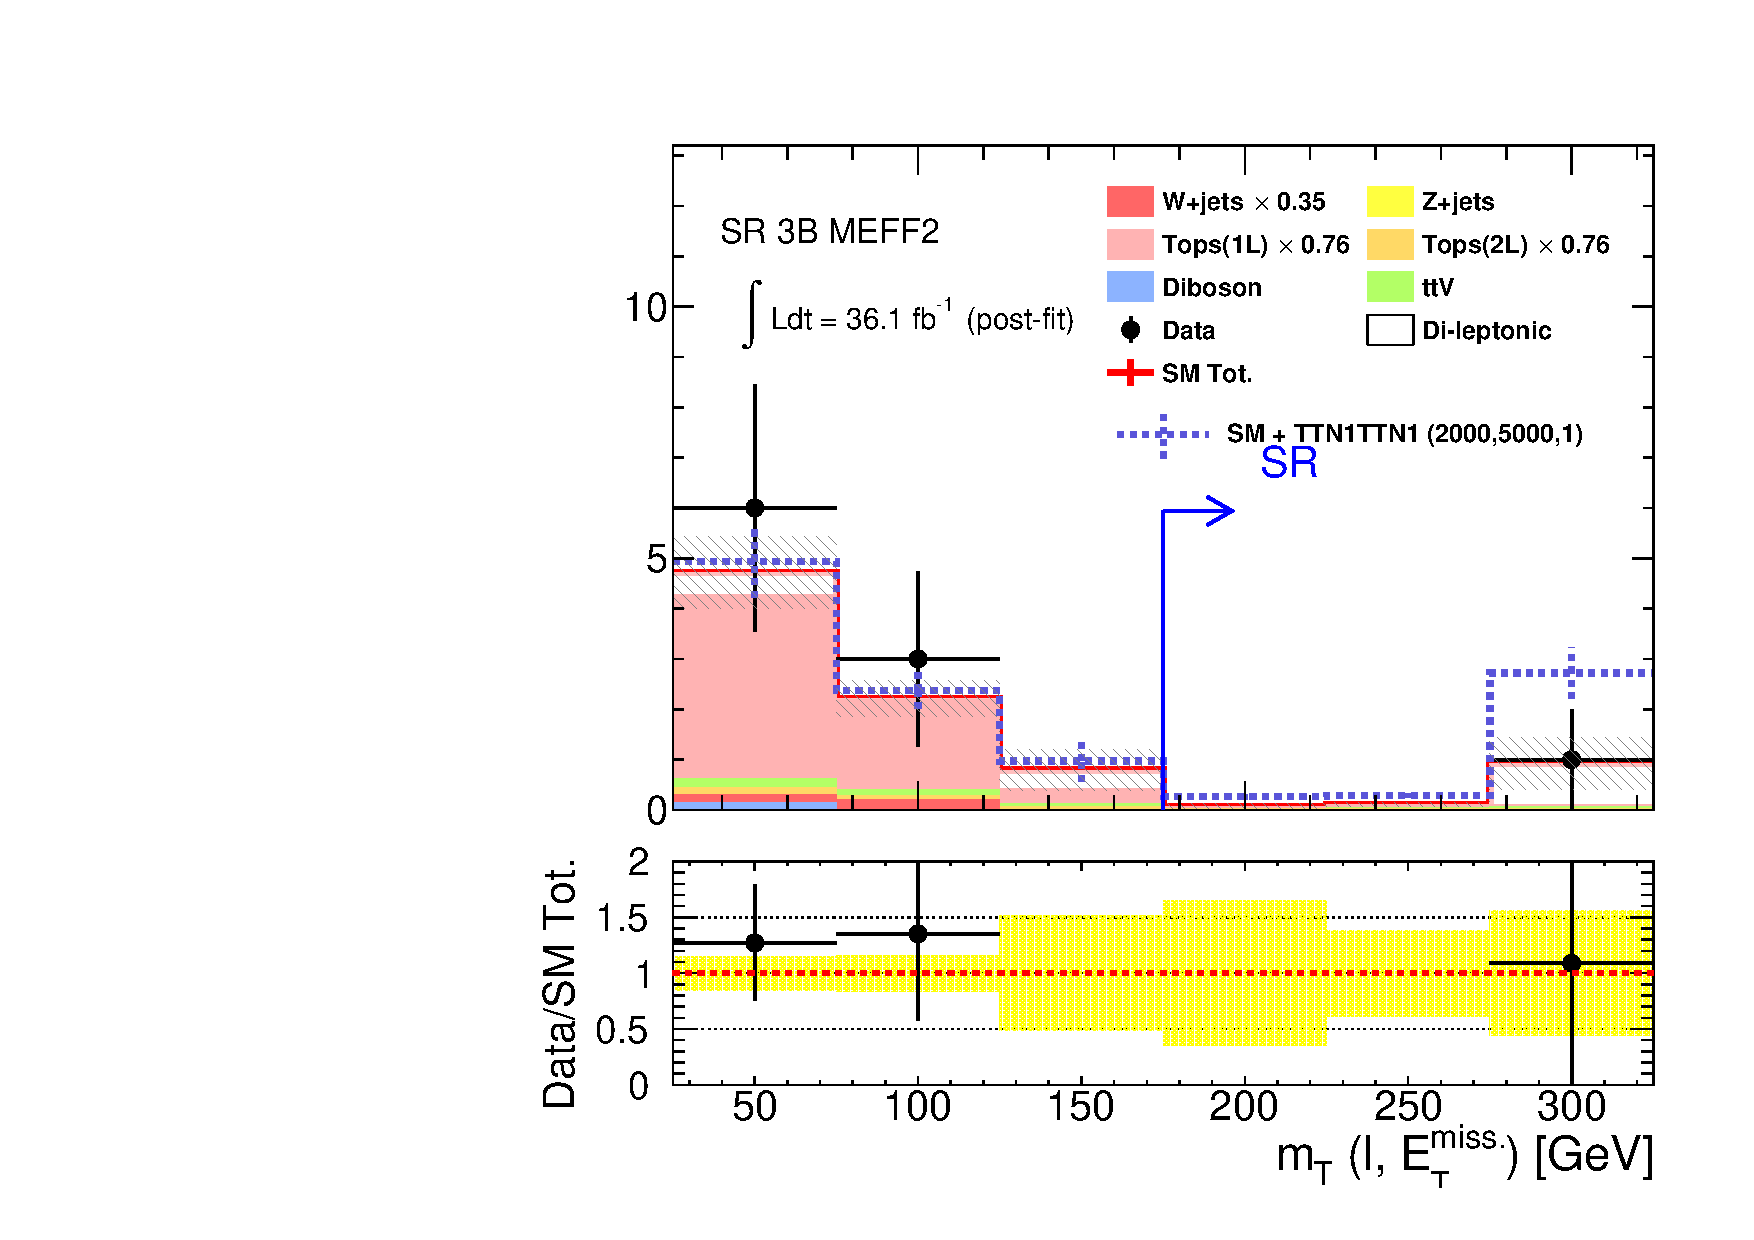
\includegraphics[width=0.41\textwidth]{figures/BGestimation/SRVRpostFit/mt__SR3BMEFF2_no_mt_postFit_2SFconfig_noYields_objRep.pdf}}
    \subfigure[]{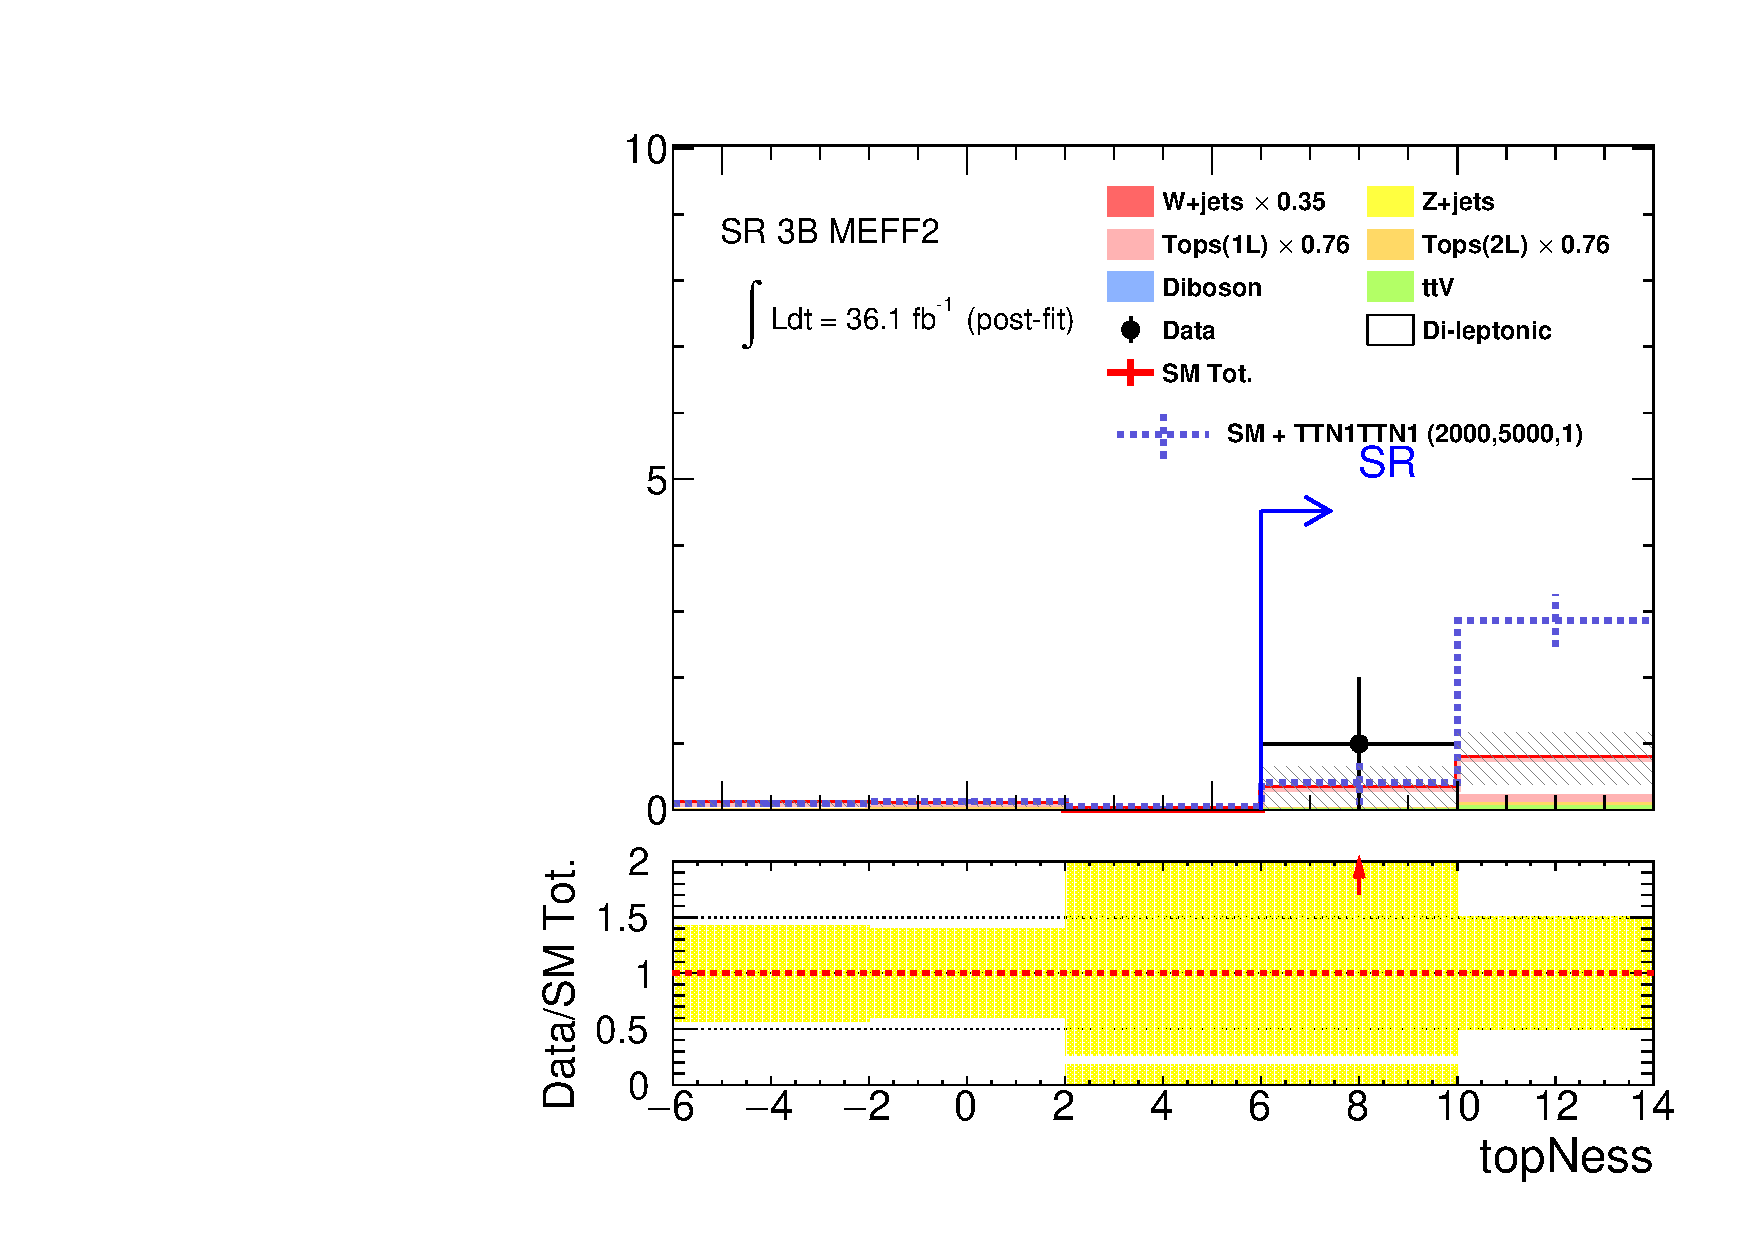
\includegraphics[width=0.41\textwidth]{figures/BGestimation/SRVRpostFit/topNess__SR3BMEFF2_no_topNess_postFit_2SFconfig_noYields_objRep.pdf}}
    \caption{   
      Post-fit distruibution of (left) $\mt$, and (right) topness.
      (a,b) SR 3B-$\meffIncFirst$.
      (c,d) SR 3B-$\meffIncSecond$.
      The yellow band in the bottom panel represents only statistical error. The overflow is included in the highest bin.  
      \label{fig::BGestimation::SRVRpostFit::SR3B}
    }
\end{figure}
